\documentclass{book}
\usepackage[hmargin = 3cm, vmargin = 2.5cm]{geometry}
\usepackage[spanish]{babel}
\usepackage{amssymb, amsmath, amsthm, graphicx, float, fancyhdr, parskip}
\usepackage[all]{xy}
\usepackage[pdfusetitle]{hyperref}

\pagestyle{fancy}
\setlength{\headheight}{25.1pt}
\fancyhf{}
\lhead[\leftmark]{}
\rhead[]{\rightmark}
\fancyfoot[LE]{\thepage}
\fancyfoot[RE]{
\includegraphics[width=0.045\textwidth]{imagenes/insta.png} \text{@jorgeroddom}}
\fancyfoot[RO]{\thepage}
\fancyfoot[LO]{
\includegraphics[width=0.045\textwidth]{imagenes/insta.png} \text{@jorgeroddom}}

\title{\Huge \textbf{Variable Compleja}}
\author{Jorge Rodríguez Domínguez}
\date{}

\newcommand{\re}{\text{Re}}
\newcommand{\im}{\text{Im}}
\newcommand{\com}{\mathbb{C}}
\newcommand{\comz}{\mathbb{C} \backslash \{0\}}
\newcommand{\argp}{\text{Arg}}
\newcommand{\logp}{\text{Log}}
\newcommand{\var}{\text{Var}}
\renewcommand{\arg}{\text{arg}}

%\definecolor{light-gray}{gray}{0.85}

%\newmdtheoremenv[backgroundcolor=light-gray]{teo}{Teorema}[section]
\newtheorem{teo}{Teorema}[section]
%\newmdtheoremenv[backgroundcolor=light-gray]{cor}[teo]{Corolario}
\newtheorem{cor}[teo]{Corolario}
%\newmdtheoremenv[backgroundcolor=light-gray]{lema}[teo]{Lema}
\newtheorem{lema}[teo]{Lema}

%\newmdtheoremenv[backgroundcolor=light-gray]{prop}[teo]{Proposición}
\newtheorem{prop}[teo]{Proposición}

\theoremstyle{definition}
%\newmdtheoremenv[backgroundcolor=light-gray]{defi}[teo]{Definición}
\newtheorem{defi}[teo]{Definición}
\newtheorem{ejemplo}[teo]{Ejemplo}
\newtheorem{obs}[teo]{Observación}

\begin{document}
% =========================================
\frontmatter
\begin{titlepage}
    \centering
    {\bfseries\LARGE \ \par}
    \vspace{1cm}{\scshape\Large \ \par}
    \vspace{3cm}
    \rule{\linewidth}{0.5mm}
    {\scshape\Huge Teoría de la Medida e Integración \par}
    \rule{\linewidth}{0.5mm} \par
    \vspace{3cm}
    {\itshape\Large Basado en las clases y apuntes de Francisco Javier Martín Reyes \par}
    \vfill
    {\Large Autor: \par}
    {\Large Jorge Rodríguez Domínguez \par}
    \vfill
\end{titlepage}

\tableofcontents

% =========================================
\mainmatter
\chapter{Introducción}

\begin{defi}
Un conjunto $\mathcal{A}$ de subconjuntos de $\Omega$ es un $\sigma$-álgebra si verifica
\begin{enumerate}
    \item[(a)] $\Omega \in \mathcal{A}$.
    \item[(b)] Si $A \in \mathcal{A}$ entonces $A^c \in \mathcal{A}$.
    \item[(c)] Si $\{A_n\}$, $A_n \in \mathcal{A}$ entonces $\cup_{n}{A_n} \in \mathcal{A}$.
\end{enumerate}
Consecuencias inmediatas
\begin{itemize}
    \item $\emptyset \in \mathcal{A}$.
    \item Si $A_n \in A$ entonces $\cap_{n}{A_n} \in \mathcal{A}$.
    \item Si $A_1,...,A_n \in \mathcal{A}$ entonces $\cup_{i=1}^{n}{A_i} \in \mathcal{A}$ y $\cap_{i=1}^{n}{A_i} \in \mathcal{A}$.
\end{itemize}
\end{defi}

\begin{defi}
Sea $\mathscr{C}$ familia de todos los intervalos. Entonces $\mathscr{C}$ define la $\sigma$-álgebra de Borel. Se denota $\mathbb{B}_1$ en $\mathbb{R}$.
\end{defi}

\begin{defi}
Sea $(\Omega, \mathcal{A})$ un espacio medible. Una probabilidad es una medida $P: \mathcal{A} \longrightarrow [0,+\infty)$ tal que
\begin{enumerate}
    \item[(1)] $P(\Omega) = 1$.
    \item[(2)] $\{A_n\}$, $A_n \in \mathcal{A}$ con $A_i \cap A_j = \emptyset$ si $i \not = j$, entonces
    \begin{align*}
        P(\cup_{n}{A_n}) = \sum_{n}{P(A_n)}.
    \end{align*}
\end{enumerate}
Consecuencias 
\begin{itemize}
    \item $P(A) = 1 - P(A^c)$, $A \in \mathcal{A}$.
    \item $P(\emptyset) = 0$.
    \item $A, B \in \mathcal{A}$ entonces $P(A \backslash B) = P(A) - P(A \cap B)$.
    \item $A, B \in \mathcal{A}$ y $A \subseteq B$ entonces $P(A) \leq P(B)$.
    \item $A, B \in \mathcal{A}$ entonces $P(A \cup B) = P(A) + P(B) - P(A \cap B)$. En general
    \begin{align*}
        P(\cup_{i=1}^{n}{A_i}) &= \sum_{i=1}^{n}{P(A_i)} - \sum_{i < j}{P(A_i \cap A_j)} + \sum_{i< j < k}{P(A_i \cap A_j \cap A_k)}\\
        & - ... + (-1)^{n-1}P(A_1 \cap ... \cap A_n).
    \end{align*}
\end{itemize}
\end{defi}

\begin{defi}
Sea $\{A_n\}$, $A_n \in \mathcal{A}$. Definimos
\begin{itemize}
    \item Límite superior de la sucesión $\{A_n\}$ como
    \begin{align*}
        \limsup_{n}{A_n} = \bigcap_{m=1}^{+\infty}{\left(\bigcup_{n=m}^{+\infty}{A_n}\right)} = A^*.
    \end{align*}
    \item Límite inferior de la sucesión $\{A_n\}$ como
    \begin{align*}
        \liminf_{n}{A_n} = \bigcup_{m=1}^{+\infty}{\left(\bigcap_{n=m}^{+\infty}{A_n}\right)} = A_*.
    \end{align*}
\end{itemize}
Consecuencias
\begin{itemize}
    \item $\liminf_{n}{A_n} \subseteq \limsup_{n}{A_n}$.
    \item Una sucesión $\{A_n\}$, $A_n \in \mathcal{A}$ es convergente si $A^* = A_*$.
\end{itemize}
\end{defi}

\begin{teo}
Sea $(\Omega, \mathcal{A})$ un espacio medible. La aplicación $P: \mathcal{A} \longrightarrow [0,+\infty)$ verificando
\begin{enumerate}
    \item[(1)] $P(\Omega) = 1$.
    \item[(2)] $A_1,...,A_n \in \mathcal{A}$ con $A_i \cap A_j = \emptyset$ si $i \not = j$, entonces
    \begin{align*}
        P(\cup_{i=1}^{n}{A_i}) = \sum_{i=1}^{n}{P(A_i)}.
    \end{align*}
    \item[(3)] Si $\{A_n\} \downarrow \emptyset$, $A_n \in \mathcal{A}$, $P(\lim_{n}{A_n}) = \lim_{n}{P(A_n)} = 0$
\end{enumerate}
Entonces $P$ es una medida de probabilidad.
\end{teo}

\begin{defi}
Sea $(\Omega, \mathcal{A})$ espacio de probabilidad. Sean $A, B \in \mathcal{A}$. A es independiente de B si $P(A \ | \ B) = P(A)$ ($P(B) > 0$).
\\
\newline
Recuérdese que
\begin{align*}
    P(A \ | \ B) = \frac{P(A \cap B)}{P(B)}, \ \ \ P(B) > 0.
\end{align*}
\end{defi}

\begin{obs}
La independencia es recírproca, es decir, $A$ es independiente de $B$ si y solo si $B$ es independiente de $A$.
\end{obs}

\begin{teo}[Teorema de la Probabilidad Compuesta]
\begin{align*}
    P(A_1 \cap ... \cap A_n) = P(A_1)P(A_2 \ | \ A_1)P(A_3 \ | \ A_1 \cap A_2)...P(A_n \ | \ A_1 \cap ... \cap A_{n-1}).
\end{align*}
\end{teo}

\begin{teo}[Teorema de la Probabilidad Total]
Sea $(\Omega, \mathcal{A}, P)$ espacio de probabilidad. Sea $\{A_n\}$ partición de $\Omega$, $P(A_n) > 0$ conocidas y sea $B \in \mathcal{A}$. Entonces
\begin{align*}
    P(B) = \sum_{n \in \mathbb{N}}{P(B \ | \ A_n)P(A_n)}.
\end{align*}
\begin{itemize}
    \item $P(A_n)$ se conoce como probabilidad a priori y $\sum_{n \in \mathbb{N}}{P(A_n)} = 1$.
    \item $P(B \ | \ A_n)$ se conocen como verosimilitudes.
\end{itemize}
\end{teo}

\begin{teo}[Teorema de Bayes]
Bajos las mismas condiciones que el teorema de la probabilidad total:
\begin{align*}
    P(A_i \ | \ B) = \frac{P(B \ | \ A_i)P(A_i)}{\sum_{n \in \mathbb{N}}{P(B \ | \ A_n)P(A_n)}} \ (\text{probabilidad a posteriori}).
\end{align*}
Y además, $\sum_{n \in \mathbb{N}}{P(A_n \ | \ B)}= 1$.
\end{teo}

\begin{obs}
\begin{itemize}
    \item $A$ es independiente de $B$ si y solo si $A$ es independiente de $B^c$ si y solo si $A^c$ es independiente de $B^c$.
    \item $\{A_1,...,A_n\}$ es una familia de sucesos independientes si cualquier $\{i_1,...,i_r\}$ verifica
    \begin{align*}
        P(A_{i_1} \cap ... \cap A_{i_r}) = \prod_{j=1}^{r}{P(A_{i_j})}.
    \end{align*}
\end{itemize}
\end{obs}
\chapter{Métodos multipaso}

\section{Motivación, ejemplos y repaso de interpolación}

\subsection{Métodos basados en integración numérica}

La solución exacta de
\begin{align*}
    \left\{ \begin{array}{lcc}
                y' = f(t,y) \\
                y(0) = y_0  \\
            \end{array}
    \right.
\end{align*}
satisface
\begin{align*}
    y(t_{k+1}) = y(t_k) + \int_{t_k}^{t_{k+1}} f(t,y(t)) \ dt.
\end{align*}
Tomando una fórmula de integración numérica para aproximar dicha integral, podemos aproximar
\begin{align*}
    y(t_{k+1}) \simeq y(t_k) +h\sum_{i=1}^{q} b_if\left( f_k^{(i)}, t_k^{(i)} \right).
\end{align*}

\begin{ejemplo}
    Método de Adams-Bashforth de 2 pasos. Si calculamos el polinomio que interpola $(t_{k-1},f_{k-1})$ y $(t_k,f_k)$, al que denotaremos por $P_1$, podemos aproximar:
    \begin{align*}
        \int_{t_{k-1}}^{t_k} f(t,y(t)) \ dt \simeq  \int_{t_{k-1}}^{t_k} P_1(t) \ dt.
    \end{align*}
    Y usando lo anterior, llegamos a que:
    \begin{align*}
        y_{k+1} = t_k + \frac{h}{2}[3f(t_k,y_k) - f(t_{k-1},y_{k-1})].
    \end{align*}
\end{ejemplo}

Para calcular los polinomios de interpolación se suelen usar la forma de Lagrange y la forma de Newton.

\subsection{Forma de Lagrange del polinomio de interpolación}

Recodemos que
\begin{align*}
    \ell_i(t) = \frac{(t-t_0) \cdots \widehat{(t - t_i)} \cdots (t - t_k)}{(t_i - t_0) \cdots \widehat{(t_i - t_i)} \cdots (t_i - t_k)},\ \ i = 1,\ldots,k.
\end{align*}
Observamos que
\begin{align*}
    \ell_i(t_j) = \left\{ \begin{array}{lcc}
                              1 & si & i = j      \\
                              0 & si & i \not = j \\
                          \end{array}
    \right.
\end{align*}
Entonces, la forma de Lagrange del polinomio de interpolación de $(t_0,f_0),\ldots,(t_k,f_k)$ es
\begin{align*}
    P_k(t) = \sum_{i=0}^{k} f_i\ell_i(t)
\end{align*}
Con esto
\begin{align*}
    \int_{a}^{b} f(t) \ dt \simeq \int_{a}^{b} P_k(t) \ dt = \int_{a}^{b} \sum_{i=0}^{k} f_i\ell_i(t) \ dt = \sum_{i=0}^{k} \alpha_i f_i
\end{align*}
siendo $\alpha_i = \int_{a}^{b} \ell_i(t) \ dt$ (pesos de la fórmula).

\subsection{Forma de Newton del polinomio de interpolación}

Recordemos que las diferencias dividas de Newton se definen como
\begin{align*}
    f[x_k]                        & = f(x_k)                                                                                  & k \in \{0,\ldots.,n\}  \\
    f[x_k,x_{k+1}]                & = \frac{f[x_{k+1}] - f[x_k]}{x_{k+1} - x_k}                                               & k \in \{0,\ldots,n-1\} \\
    f[x_k,x_{k+1},x_{k+2}]        & = \frac{f[x_{k+1},x_{k+2}] - f[x_k,x_{k+1}]}{x_{k+2} - x_k}                               & k \in \{0,\ldots,n-2\} \\
                                  & \vdots                                                                                                             \\
    f[x_k,x_{k+1},\ldots,x_{k+i}] & = \frac{f[x_{k+1},x_{k+2},\ldots,x_{k+1}] - f[x_k,x_{k+1},\ldots,x_{k+i-1}]}{x_{k+i}-x_k} & k \in \{0,\ldots,n-i\}
\end{align*}
De esta manera, la forma de Newton del polinomio de interpolación de $(t_0,f_0),\ldots,(t_k,f_k)$ es
\begin{align*}
    P_k(t) = f_0 + f[t_0,t_1](t-t_0) + f[t_0,t_1,t_2](t-t_0)(t-t_1) + \ldots + f[t_0,\ldots,t_k](t-t_0)\cdots(t-t_{k-1})
\end{align*}
Aunque en la práctica usaremos la otra expresión, que viene dada por:
\begin{align*}
    P_k(t) = f_k & + f[t_{k-1},t_k](t-t_k) + f[t_{k-2},t_{k-1},t_k](t-t_k)(t-t_{k-1}) + \ldots \\
                 & + f[t_0,\ldots,t_k](t-t_k)\cdots (t-t_1)
\end{align*}

\begin{defi}[Diferencias finitas regresivas]
    La diferencia finita regresiva de orden 0 en $t_j$ es $\bigtriangledown^0f_j = f_j$. De forma recursiva, definimos:
    \begin{align*}
        \bigtriangledown^{k+1}f_k = \bigtriangledown^k f_j - \bigtriangledown^kf_{j-1}.
    \end{align*}
\end{defi}

\begin{obs}
    De esta manera, tenemos que
    \begin{align*}
        f[t_i,\ldots,t_{i+j}] = \frac{\bigtriangledown^j f_{i+j}}{j! h^j}.
    \end{align*}
    Con lo que podemos reeescribir la forma de Newton del polinomio de interpolacón como
    \begin{align*}
        P_k(t) = \widetilde{P}_k(s) = \bigtriangledown^0 f_k + \bigtriangledown^1 f_k + \frac{\bigtriangledown^2 f_k}{2!}s(s+1) + \ldots + \frac{\bigtriangledown^k f_k}{k!}s(s+1)\cdots (s+k-1).
    \end{align*}
    siendo $sh = t - t_k$. Observamos que
    \begin{align*}
        \binom{s}{j} = \frac{s!}{j!(s-j)!} = \frac{s(s-1) \cdots (s-k+1)}{j!},
    \end{align*}
    con lo que
    \begin{align*}
        \boxed{
            P_k(t) = \widetilde{P}_k(s) = \sum_{i=0}^{k} \binom{s+i-1}{i} \bigtriangledown^i f_k, \ \ \ s = \frac{t - t_k}{h}.
        }
    \end{align*}
    Esta expresión se conoce como la expresión de Gregory-Newton regresiva del polinomio de interpolación.
\end{obs}

\section{Métodos multipaso basados en integración numérica}

\subsection{Métodos de Adams-Bashforth}

La solución exacta de la ecuación $y' = f(t,y)$ verifica que
\begin{align*}
    y(t_{k+1}) = y(t_k) + \int_{t_k}^{t_{k+1}} f(t,y(t)) \ dt.
\end{align*}
La idea del métodos de Adams-Bashforth de $q$ pasos es aproximar:
\begin{align*}
    \int_{t_k}^{t_{k+1}} f(t,y(t)) \ dt \thickapprox \int_{t_k}^{t_{k+1}} P_{q-1}(t) \ dt.
\end{align*}
siendo $P_{q-1}$ el polinomio de interpolación de $(t_k,f_k),\ldots,(t_{k-q+1},f_{k-q+1})$.

La expresión del método $AB$ de $q$ pasos es la siguiente:
\begin{align*}
    t_{k+1} = t_k + \int_{t_k}^{t_{k+1}} P_{q-1}(t) \ dt.
\end{align*}
Si hacemos el cambio de variable $s = \frac{t - t_k}{h}$, entonces:
\begin{align*}
    \boxed{
        y_{k+1} = y_k + h \int_{0}^{1} \widetilde{P}_{q-1}(s) \ ds.
    }
\end{align*}

\begin{ejemplo} \
    \begin{enumerate}
        \item La expresión del método $AB1$ es:
              \begin{align*}
                  y_{k+1} = y_k + hf_k.
              \end{align*}
        \item La expresión del método $AB2$ es:
              \begin{align*}
                  y_{k+1} = y_k + \frac{h}{2}(3f_k - f_{k-1}).
              \end{align*}
        \item La expresión del método $AB3$ es:
              \begin{align*}
                  y_{k+1} = y_k + \frac{h}{12}(23f_k - 16f_{k-1} +5f_{k-2}).
              \end{align*}
    \end{enumerate}
\end{ejemplo}

\subsection{Métodos de Adams-Moulton}

Los métodos Adams-Moulton son métodos implícitos. Dichos métodos son parecidos a los Adams-Bashfort, pero vamos a usar el polinomio de interpolación $Q_q$ que interpola los puntos
\begin{align*}
    (t_{k+1},f_{k+1}),(t_k,f_k),\ldots,(t_{k-q+1},f_{k-q+1}),
\end{align*}
es decir, usamos en la expresión del polinomio a $f_{k+1}$, que para conocerlo necesitamos $y_{k+1}$ (por eso es un método implícito). El método de Adams-Moulton de $q$ pasos es:
\begin{align*}
    \boxed{
        y_{k+1} = y_k + h\int_{-1}^{0} \widetilde{Q}_q (s) \ ds, \ \ \ s = \frac{t - t_k}{h}.
    }
\end{align*}

\begin{ejemplo} \
    \begin{enumerate}
        \item La expresión del método $AM1$ (o método del trapecio) es:
              \begin{align*}
                  y_{k+1} = y_k + \frac{h}{2}(f_{k+1} + f_k).
              \end{align*}
        \item La expresión del método $AM2$ es:
              \begin{align*}
                  y_{k+1} = y_k +\frac{h}{12}(5f_{k+1} + 8f_{k} - f_{k-1}).
              \end{align*}
    \end{enumerate}
\end{ejemplo}

\section{Métodos BDF}
Los métodos BDF (en inglés, \textit{Backward differentiation formula}) son métodos basados en diferenciación numérica. Supongamos que conocemos el valor de la función $y(t)$ en $k+1$ puntos y queremos aproximar $y'(\overline{t})$. Una aproximación razonable es $y(\overline{t}) \thickapprox P_k'(\overline{t})$, siendo $P_k$ el polinomio de interpolación de $(t_0,y(t_0)),\ldots,(t_k,f(t_k))$.

El método $BDF$ de $q$ pasos viene dado por
\begin{align*}
    \frac{1}{h} \widetilde{R}'_q(0) = f(t_{k+1},y_{k+1})
\end{align*}
siendo $R_q$ el polinomio que interpola $(t_{k+1},y_{k+1}),\ldots,(t_{k-q+1},y_{k-q+1})$.

\begin{ejemplo} \
    \begin{enumerate}
        \item La expresión del método $BDF1$ es:
              \begin{align*}
                  y_{k+1} = y_k + hf(t_{k+1},y_{k+1}),
              \end{align*}
              es decir, coincide con Euler implícito.
        \item La expresión del método $BDF2$ es:
              \begin{align*}
                  y_{k+1} -\frac{4}{3}y_k + \frac{1}{3}y_{k-1} = \frac{2h}{3}f(t_{k+1},y_{k+1})
              \end{align*}
    \end{enumerate}
\end{ejemplo}

\section{Análisis de los métodos multipaso}

Todos los métodos multipaso se puede escribir de la forma:
\begin{align*}
    \sum_{i=0}^{q} \alpha_i y_{k+i} = h\sum_{i=0}^{q} \beta_i f_{k+i}
\end{align*}

\begin{obs}
    Para que un método multipaso tenga $q$ pasos ha de ocurrir que:
    \begin{itemize}
        \item $\alpha_q \not = 0$.
        \item $|\alpha_0| + |\beta_0| > 0$.
    \end{itemize}
    Si $\beta_q = 0$, entonces tenemos un método explícito.
\end{obs}

\subsection{Orden y consistencia}

\begin{defi}
    Error en $t_k$ es $e_k = |y(t_k) - y_k|$.
\end{defi}
\begin{defi}
    Error es $e(h) = \max_{k} e_k$.
\end{defi}

\begin{defi}
    Definimos el error de discretización local en $t_{k+q}$ como $\varepsilon_{k+1} = y(t_{k+q}) - \widetilde{y}_{k+q}$, siendo $\widetilde{y}_{k+q}$ tal que:
    \begin{align*}
        \alpha_q \widetilde{y}_{k+q} + \sum_{i=0}^{q-1} \alpha_i y(t_{k+i}) = h\beta_q f(t_{k+q},\widetilde{y}_{k+q}) + h\sum_{i=0}^{q-1} \beta_i f(t_{k+i},y(y_k+i)).
    \end{align*}
\end{defi}

\begin{defi}
    Se dice que el método es consistente si
    \begin{align*}
        \lim_{h \to 0} \sum_{k=0}^{N - q} |\varepsilon_{k+q}| = 0.
    \end{align*}
\end{defi}

\begin{defi}
    Se dice que el método es de orden $p$ si $\varepsilon_{q+k} = O(h^{p+1})$, $k=0,1,2,\ldots$, para cualquier solución $y(t)$ de clase $\mathcal{C}^{p+1}$.
\end{defi}

\begin{defi}
    Dado un método de $q$ pasos
    \begin{align*}
        \sum_{i=0}^{q} \alpha_i y_{k+i} = h\sum_{i=0}^{q} \beta_i f_{k+i}
    \end{align*}
    se define el \textbf{operador diferencia} de la siguiente manera: Dada $y:[t_0,t_0+T] \longrightarrow \mathbb{R}$ derivable, dado $h>0$, dado $t \in [t_0,t_0+T-qh]$, el operador diferencia viene dado por
    \begin{align*}
        L(y,t,h) = \sum_{i=0}^{q}[\alpha_i y(t+ih) - h\beta_i y'(t+ih)].
    \end{align*}
\end{defi}

\begin{teo}
    El método
    \begin{align*}
        \sum_{i=0}^{q} \alpha_i y_{k+i} = h\sum_{i=0}^{q} \beta_i f_{k+i}
    \end{align*}
    es orden $p$ si y solo si $L(y,t,h) = O(h^{p+1})$ para cualquier $y \in \mathcal{C}^{p+1}([t_0,t_0+T])$.
\end{teo}

\begin{teo}
    El método multipaso
    \begin{align*}
        \sum_{i=0}^{q} \alpha_i y_{k+i} = h\sum_{i=0}^{q} \beta_i f_{k+i}
    \end{align*}
    es orden al menos $p$ si y solo si
    \begin{itemize}
        \item $\sum_{i=0}^{q} \alpha_i = 0$.
        \item $\sum_{i=0}^{q} \alpha_i i^l = l\sum_{i=0}^{q} \beta_i i^{l-1}$, $l = 1,\ldots,p$.
    \end{itemize}
\end{teo}

\begin{proof}
    Sea $y \in \mathcal{C}^{p+1}([t_0,t_0+T])$ y $h > 0$.  Hemos de probar que
    \begin{align*}
        L(y,t,h) = \sum_{i=0}^{q}[\alpha_i y(t+ih) - h\beta_i y'(t+ih)] = O(h^{p+1}).
    \end{align*}
    Desarrollando el polinomio de Taylor de $y$ y evaluando en $t+ih$:
    \begin{align*}
        y(t+ih) & = y(t) + y'(t)ih + y''(t)\frac{(ih)^2}{2} + \ldots + y^{(p)}(t)\frac{(ih)^p}{p!} + O(h^{p+1}) \\
                & = \sum_{l=0}^{p} \frac{y^{(l)}(t)}{l!}i^lh^l + O(h^{p+1}).
    \end{align*}
    Actuando de forma análoga con $y'$:
    \begin{align*}
        hy'(t+ih) & = y'(t)h + y''(t)ih + y'''(t)\frac{i^2h^3}{2} + \ldots + y^{(p)}(t)\frac{i^{p-1}h^p}{(p-1)!} + O(h^{p+1}) \\
                  & = \sum_{l=1}^{p} \frac{y^{(l)}(t)}{(l-1)!}i^{l-1}h^l + O(h^{p+1}).
    \end{align*}
    Con esto llegamos que
    \begin{align*}
        L(y,t,h) & = \sum_{i=0}^{q} \left[ \alpha_i \sum_{l=0}^{p} \frac{y^{(l)}(t)}{l!}i^lh^l - \beta_i \sum_{l=1}^{p} \frac{y^{(l)}(t)}{(l-1)!}i^{l-1}h^l \right] + O(h^{p+1})        \\
                 & = \left( \sum_{i=0}^{q} \alpha_i \right) y(t) + \sum_{l=1}^{p} \frac{y^{(l)}(t)}{l!}h^l\left( \sum_{i=0}^{q} \alpha_i i^l - l\sum_{i=0}^{q} \beta_i i^{l-1} \right).
    \end{align*}
    Luego, $L(t,y,h) = O(h^{p+1})$ si y solo si
    \begin{itemize}
        \item $\sum_{i=0}^{q} \alpha_i = 0$.
        \item $\sum_{i=0}^{q} \alpha_i i^l = l\sum_{i=0}^{q} \beta_i i^{l-1}$, $l = 1,\ldots,p$.
    \end{itemize}
\end{proof}

\begin{prop}
    El método de Adams-Moulton de $q$ pasos tiene orden $q+1$.
\end{prop}

\subsection{Estabilidad}
Antes de comenzar con la estabilidad, necesitmos recordar las ecuaciones en diferencias lineales homogéneas y de coeficientes constantes. Supongamos que tenemos la siguiente ecuación:
\begin{align*}
    \alpha_q y_{k+q} + \alpha_{q-1} y_{k+q-1} \ldots + \alpha_0 y_k = 0, \ \ k = 0,1,2,\ldots \ \ \alpha_1,\ldots,\alpha_q \in \mathbb{R}, \ \ \alpha_q \not = 0
\end{align*}
Una sucesión $\{y_k\}_{k=0}^{\infty}$ es solución si satisface dicha ecuación. El conjunto de soluciones tiene estructura de espacio vectorial de dimensión $q$. Una base es:

\begin{align*}
    \left\{ \begin{array}{lcc}
                y_0^0 = 1,\ y_1^0 = 0,\ \ldots,\ y_{q-1}^0 = 0,\ y_q^0,\ y_{q+1}^0,\ \ldots                     \\
                \\ y_0^1 = 0,\ y_1^1 = 1,\ \ldots,\ y_{q-1}^1 = 0,\ y_q^1,\ y_{q+1}^1,\ \ldots\\
                \vdots                                                                                          \\
                y_0^{q-1} = 0,\ y_1^{q-1} = 0,\ \ldots,\ y_{q-1}^{q-1} = 1,\ y_q^{q-1},\ y_{q+1}^{q-1},\ \ldots \\
            \end{array}
    \right.
\end{align*}
Para resolver la ecuación en diferencias finitas, hemos de encontrar una expresión de $y_k$. ¿Existen soluciones de la forma $\{\lambda^k\}_{k=0}^{\infty}$ con $\lambda \in \mathbb{R} \backslash \{0\}$?
\begin{align*}
    0 = \alpha_q \lambda^{k+q} + \ldots+ \alpha_1 \lambda^{k+1} + \alpha_0 \lambda^{k} = \lambda^k[\alpha_q \lambda^{q} + \ldots + \alpha_1 \lambda + \alpha_0] \Longleftrightarrow \alpha_q \lambda^{q} + \ldots + \alpha_1 \lambda + \alpha_0 = 0.
\end{align*}
Denotaremos $p(\lambda) = \alpha_q \lambda^{q} + \ldots + \alpha_1 \lambda + \alpha_0$. Distinguimos los siguientes casos:
\begin{enumerate}
    \item Si $p(\lambda)$ tiene $q$ raíces reales y distintas $\lambda_1,\ldots,\lambda_q$. Entonces todas las soluciones puede escribirse de la forma
          \begin{align*}
              y_k = c_1\lambda_1^k + \ldots + c_q \lambda_q, \ \ c_1,\ldots,c_q \in \mathbb{R}.
          \end{align*}
          En este caso, podemos afirmar que todas las soluciones de la ecuación en diferencias están acotadas si $|\lambda_i| \leq 1$ para cada $i = 1,\ldots,q$.
    \item Si $p(\lambda)$ tiene una raíz $\lambda$ con multiplicidad $m$, entonces es fácil comprobar que las sucesiones:
          \begin{align*}
              \{\lambda^k\}_{k=0}^{\infty}, \ \{k\lambda^k\}_{k=0}^{\infty},\ \ldots,\{k^{m-1}\lambda^k\}_{k=0}^{\infty}.
          \end{align*}
          son soluciones de la ecuación y son linealmente independientes. Por tanto, también será solución una combinación lineal de ellas, es decir: \begin{align*}
              y_k = \beta_1 \lambda^k + \beta_2 k \lambda^k + \ldots +\beta_m k^{m-1}\lambda^k = Q(k)\lambda^k, \ \ \alpha_1,\ldots,\alpha_m \in \mathbb{R},
          \end{align*}
          siendo $Q$ un polinomio de grado menor o igual que $m-1$. Luego, si $\lambda$ es raíz real de multiplicidad $m$, son soluciones:
          \begin{align*}
              y_k = Q(k)\lambda^k,
          \end{align*}
          con $Q$ polinomio de grado menor o igual que $m-1$. En este caso, podemos afirmar que todas las soluciones de la ecuación en diferencias están acotadas si $|\lambda| < 1$ o $|\lambda| = 1$ pero $m=1$.
    \item Si $p(\lambda)$ tiene un par de raíces complejas (conjugadas). Sean $\mu_{\pm} = \alpha e^{\pm i \theta} = \alpha(\cos \theta \pm i\sen\theta)$ dichas raíces complejas. Es fácil comprobar que:
          \begin{align*}
              \{\alpha^k \cos(k\theta) \}_{k=0}^{\infty}, \ \{\alpha^k \sen(k\theta) \}_{k=0}^{\infty},
          \end{align*}
          son soluciones de la ecuación y son linealmente independientes. Por tanto, es solución una combinación lineal de ellas, es decir:
          \begin{align*}
              y_k = \alpha^k(c_1 \cos(k\theta) + c_2 \sen(k\theta)).
          \end{align*}
          En este caso, podemos afirmar que todas las soluciones de la ecuación en diferencias están acotadas si $|\alpha| \leq 1$.
    \item Si $p(\lambda)$ tiene al par de raíces comeplejas $\mu_{\pm} = \alpha e^{\pm i \theta} = \alpha(\cos \theta \pm i\sen\theta)$ con multiplicidad $m$, entonces
          \begin{align*}
              y_k = \alpha^k(R_1(k)\cos(k\theta) + R_2(k)\sen(k\theta)),
          \end{align*}
          siendo $P$ y $Q$ polinomios de grado menor o igual que $m-1$. En este caso, podemos afirmar que todas las soluciones de la ecuación en diferencias están acotadas si $|\alpha| < 1$ o $|\alpha = 1|$ pero $m = 1$.

\end{enumerate}
En conclusión: Todas las soluciones de la ecuación en diferencias están acotadas si y solo las raíces $\lambda$ de $p$ sastisfacen una de las siguientes condiciones:
\begin{itemize}
    \item $|\lambda| < 1$.
    \item $|\lambda| = 1$ y multiplicidadad 1.
\end{itemize}
(si $\lambda$ es complejo, $|\lambda|$ es su módulo).

\begin{defi}
    Dado un método multipaso
    \begin{align*}
        \sum_{i=0}^{q} \alpha_i y_{k+i} = h\sum_{i=0}^{q} \beta_i f_{k+i},
    \end{align*}
    se denomina
    \begin{itemize}
        \item Primer polinomio característico a:
              \begin{align*}
                  \rho(s) = \sum_{i=0}^{q} \alpha_i s^i.
              \end{align*}
        \item Segundo polinomio característico a:
              \begin{align*}
                  \sigma(s) = \sum_{i=0}^{q} \beta_i s^i.
              \end{align*}
    \end{itemize}
\end{defi}

\begin{defi}
    Se dice que el método verifica la condición de la raíz si todas las raíces $\lambda$ del primer polinomio característico verifican una de las siguientes condiciones:
    \begin{itemize}
        \item $|\lambda| < 1$.
        \item $|\lambda| = 1$ y multiplicidadad 1.
    \end{itemize}
\end{defi}

\begin{teo}
    Un método multipaso es estable si y solo si se verifica la condición de la raíz.
\end{teo}

\begin{obs}
    Si el método es consistente, entonces $\lambda = 1$ es siempre raíz del primer polinomio característico pues:
    \begin{align*}
        \rho(1) = \alpha_0 + \ldots + \alpha_q = 0
    \end{align*}
    Para que sea estable, tiene que tener multiplicidad 1.
\end{obs}

\begin{ejemplo} \
    \begin{enumerate}
        \item Los métodos Adams (AM ó AB) son todos estables.
        \item Los métodos BDF son estables para $q = 1,\ldots,6$.
    \end{enumerate}
\end{ejemplo}

\begin{teo}[Primera barrera de Dahlquist] \
    \begin{itemize}
        \item Un método multipaso estable de $q$ pasos tiene a lo sumo orden $q+1$ si $q$ es impar o $q+2$ si $q$ es par.
        \item Si además es explícito, su orden es a lo sumo $q$.
    \end{itemize}
\end{teo}

\begin{teo}
    Un método multipaso que satisface:
    \begin{itemize}
        \item La codición de la raíz.
        \item $\alpha_0 + \ldots + \alpha_q = 0$.
        \item $\sum_{i=0}^{q} \alpha_i i^l = l\sum_{i=0}^{q} \beta_i i^{l-1}$, $l = 1,\ldots,p$.
    \end{itemize}
    es convergente. Si además el método es de orden $p$ y los $q$ primeros pasos se dan con un método unipaso de orden $p$, entonces existe $c > 0$ (independiente de $h$) tal que:
    \begin{align*}
        \max_{i=0,\ldots,N} |y(t_i) - y_i| \leq ch^p.
    \end{align*}
\end{teo}
\chapter{Integración de funciones medibles}

El objetivo de este tema es construir la integral asociada a una medida. Recordamos las ideas intuitivas introducidas en el primer tema. Éstas nos llevan a la conclusión de que, dado un espacio de medida $(X, \mathcal{M}, \mu)$, las funciones $f: X \longrightarrow \mathbb{R}$ susceptibles de ser integradas son aquellas que verifican que $f^{-1}([a, b))$ es un conjunto medible, es decir $f^{-1}([a, b)) \in \mathcal{M}$, cualquiera que sea el intervalo acotado $[a, b)$. Dicho de otro modo, las funciones con las que vamos a trabajar son las funciones medibles que han sido estudiadas en el capítulo anterior.
\\
\newline
Para construir la integral, procederemos de acuerdo con los pasos siguientes: en primer lugar, definimos la integral de una función simple, medible, no negativa, luego la de una función medible no negativa arbitraria y después la de las funciones medibles reales y complejas. 

\section{Integración de funciones simples, medibles y no negativas}

\subsection{La integral sobre el conjunto completo $X$}

\begin{defi}
Sean $(X, \mathcal{M}, \mu)$ un espacio de medida y $\varphi: X \longrightarrow [0, +\infty)$ una función simple y medible de expresión canónica
\begin{align*}
    \varphi = \sum_{i=1}^{n}{a_i \mathcal{X}_{A_i}}.
\end{align*}
Definimos la integral de $\varphi$ en $X$ (o sobre $X$) respecto de la medida $\mu$, y la denotamos por $\int_{X}{\varphi} \ d\mu$, mediante
\begin{align*}
    \int_{X}{\varphi \ d\mu} := \sum_{i=1}^{n}{a_i\mu(A_i)}.
\end{align*}
Observemos que, como $\varphi \ge 0$, se tiene que $\int_{X}{\varphi} \ d\mu \ge 0$ y que $\int_{X}{\varphi} \ d\mu$ puede ser igual a $+\infty$. 
\\
\newline
Para esta integral, usaremos también otras notaciones como las siguientes:
\begin{align*}
    \int_{X}{\varphi}, \ \ \ \int_{X}{\varphi(x) \ d\mu(x)}, \ \ \ \int{\varphi}.
\end{align*}
\end{defi}
Como la definición de la integral depende de la expresión canónica, en estos primeros momentos tenemos que trabajar exclusivamente con la expresión canónica de $\varphi$. Para que el desarrollo sea más sencillo, vamos a establecer una proposición.

\begin{prop}
Sea $\varphi: X \longrightarrow [0,+\infty)$ una función simple y medible de expresión
\begin{align*}
    \varphi = \sum_{j=1}^{l}{d_j \mathcal{X}_{D_j}},
\end{align*}
donde $d_j \ge 0$, $d_j \in \mathbb{R}$, $D_j \in \mathcal{M}$, $D_i \cap D_j = \emptyset$ si $i \not = j$ y $\bigcup_{j=1}^{l}{D_j} = X$. Entonces
\begin{align*}
    \int_{X}{\varphi \ d\mu} = \sum_{j=1}^{l}{d_j \mu(D_j)}.
\end{align*}
\end{prop}

\begin{proof}
Sea
\begin{align*}
    \varphi = \sum_{i=1}^{n}{a_i \mathcal{X}_A}
\end{align*}
la expresión canónica de la función simple. Entonces
\begin{align*}
    \int_{X}{\varphi \ d\mu} = \sum_{i=1}^{n}{a_i\mu(A_i)}.
\end{align*}
Como $X = \bigcup_{j=1}^{l}{D_j}$, entonces $A_i = \bigcup_{j=1}^{l}{(A_i \cap D_j)}$ y, por ser la unión disjunta
\begin{align*}
    \int_{X}{\varphi \ d\mu} &= \sum_{i=1}^{n}{a_i\mu(A_i)} = \sum_{i=1}^{n}{a_i\mu \left(\bigcup_{j=1}^{l}{A_i \cap D_j}\right)} = \sum_{i=1}^{n}{ \left( a_i \sum_{j=1}^{l}{\mu(A_i \cap D_j)}\right)}\\ 
    &= \sum_{i=1}^{n}{\sum_{j=1}^{l}{a_i\mu(A_i \cap D_j)}}
\end{align*}
Es claro que $a_i \mu(A_i \cap D_j) = d_j \mu(A_i \cap D_j)$. Entonces,
\begin{align*}
    \int_{X}{\varphi \ d\mu} &= \sum_{i=1}^{n}{\sum_{j=1}^{l}{a_i\mu(A_i \cap D_j)}} = \sum_{i=1}^{n}{\sum_{j=1}^{l}{d_j\mu(A_i \cap D_j)}} = \sum_{j=1}^{n}{ \left( d_j\sum_{i=1}^{n}{\mu(A_i \cap D_j)} \right)}\\
    &= \sum_{j=1}^{l}{d_j \mu(D_j)}.
\end{align*}
donde en la penútlima igualdad hemos usado que los conjuntos $A_i$ forman un partición de $X$.
\end{proof}

\begin{obs}
\begin{enumerate}
    \item[(1)] Si $\varphi = c \mathcal{X}_E$, $c \ge 0$, $E \in \mathcal{M}$,
    \begin{align*}
        \int_{X}{\varphi \ d\mu} = c\mu(E).
    \end{align*}
    En efecto, $\varphi = c \mathcal{X}_E + 0 \mathcal{X}_{X \backslash E}$ y, en consecuencia, por la proposición anterior
    \begin{align*}
        \int_{X}{\varphi \ d\mu} = c\mu(E) + 0\mu(X \backslash E) = c\mu(E).
    \end{align*}
    \item[(2)] Si $\varphi = 0 \ (= 0 \mathcal{X}_X)$
    \begin{align*}
        \int_{X}{\varphi \ d\mu} = 0.
    \end{align*}
    \item[(3)] Si $\varphi = 1 \ (= \mathcal{X}_X)$
    \begin{align*}
        \int_{X}{\varphi \ d\mu} = \mu(X).
    \end{align*}
\end{enumerate}
\end{obs}
\begin{prop}
Sean $\varphi, \psi : X \longrightarrow [0,+\infty)$ simples y medibles. Entonces $\varphi + \psi$ es una función simple, medible y
\begin{align*}
    \int_{X}{(\varphi + \psi) \ d\mu} = \int_{X}{\varphi \ d\mu} + \int_{X}{\psi \ d\mu}.
\end{align*}
\end{prop}

\begin{proof}
Consideremos las expresiones canónicas de $\varphi$ y $\psi$,
\begin{align*}
    \varphi = \sum_{i=1}^{n}{a_i \mathcal{X}_{A_i}}, \ \ \ \psi = \sum_{j=1}^{s}{b_i \mathcal{X}_{B_j}}.
\end{align*}
Por lo tanto, si $i \not = j$ tenemos que $a_i \not = a_j$, $b_i \not = b_j$, $A_i \cap A_j = \emptyset$, $B_i \cap B_j = \emptyset$. Además $\bigcup_{i=1}^{n}{A_i} = X$ y $\bigcup_{j=1}^{s}{B_j} = X$. Así,
\begin{align*}
    X = \bigcup_{i=1}^{n}{A_i \cap X} = \bigcup_{i=1}^{n}{A_i \cap \left( \bigcup_{j=1}^{s}{B_j} \right)} = \bigcup_{i=1}^{n}{ \left( \bigcup_{j=1}^{s}{A_i \cap B_j} \right)} = \bigcup_{i,j=1}^{n,s}{A_i \cap B_j},
\end{align*}
y esta unión es disjunta (es decir, los conjuntos $\{ A_i \cap B_j\}_{i,j=1}^{n,s}$ son disjuntos dos a dos). Claramente,
\begin{align*}
    \varphi + \psi = \sum_{i,j=1}^{n,s}{(a_i + b_j)\mathcal{X}_{A_i \cap B_j}}.
\end{align*}
Por lo tanto, por la proposición anterior
\begin{align*}
    \int_{X}{\varphi + \psi \ d\mu} &= \sum_{i,j = 1}^{n,s}{(a_i + b_j)\mu(A_i \cap B_j)}\\
    &= \sum_{i=1}^{n}{\sum_{j=1}^{s}{(a_i\mu(A_i \cap B_j) + b_j\mu(A_i \cap B_j))}}\\
    &=\sum_{i=1}^{n}{ \left( a_i \sum_{j=1}^{s}{\mu(A_i \cap B_j)} \right)} + \sum_{j=1}^{s}{ \left( b_j\sum_{i=1}^{n}{\mu(A_i \cap B_j)} \right)}\\
    &= \sum_{i=1}^{n}{a_i\mu(A_i)} + \sum_{j=1}^{s}{b_j\mu(B_j)} = \int_{X}{\varphi \ d\mu} + \int_{X}{\psi \ d\mu}.
\end{align*}
donde, en las útlimas igualdades, hemos usado que $\mu$ es una medida.
\end{proof}

\begin{obs}
\begin{enumerate}
    \item[(1)] Es obvio que, por inducción, la anterior igualdad se extiende a cualquier número finito de funciones simples medibles.
    \item[(2)] Supongamos que $E_1, ..., E_n \in \mathcal{M}$ y $c_1, ...,c_n \ge 0$, $c_i \in \mathbb{R}$, entonces la función $\varphi = \sum_{i=1}^{n}{c_i \mathcal{X}_{E_i}}$ es simple aunque, probablemente, la expresión anterior no sea la canónica ni los conjuntos $E_i$ sean una partición de $X$. Sin embargo, se tiene que
    \begin{align*}
        \int_{X}{\varphi \ d\mu} = \int_{X}{\left(  \sum_{i=1}^{n}{c_i \mathcal{X}_{E_i} \ d\mu}\right)} = \sum_{i=1}^{n}{c_i\mu(E_i)}.
    \end{align*}
    En efecto, utilizando la aditividad que acabamos de demostrar y que sabemos que $\int_{c}{\mathcal{X}_E}} = c\mu(E)$, obtenemos
    \begin{align*}
        \int_{X}{\left(  \sum_{i=1}^{n}{c_i \mathcal{X}_{E_i}}\right) d\mu} = \sum_{i=1}^{n}{\left( \int_{X}{c_i \mathcal{X}_{E_i} \ d\mu} \right)} = \sum_{i=1}^{n}{c_i\mu(E_i)}.
    \end{align*}
\end{enumerate}
\end{obs}
\begin{prop}
Si $\varphi: X \longrightarrow [0,+\infty)$ es medible y simple y $c \ge 0$ $(c \in \mathbb{R})$, entonces $c\varphi$ es simple, medible y
\begin{align*}
    \int_{X}{c\varphi \ d\mu} = c\int_{X}{\varphi \ d\mu}.
\end{align*}
\end{prop}

\begin{proof}
Sea $\varphi = \sum_{i=1}^{n}{c_i \mathcal{X}_{E_i}}$. Entonces
\begin{align*}
    \int_{X}{c\varphi \ d\mu} &= \int_{X}{\left( \sum_{i=1}^{n}{cc_i \mathcal{X}_{E_i}} \right) d\mu} = \sum_{i=1}^{n}{\left( \int_{X}{cc_i \mathcal{X}_{E_I} \ d\mu} \right)} =  \sum_{i=1}^{n}{cc_i\mu(E_i)} = \\
    &= c \left( \sum_{i=1}^{n}{c_i\mu(E_i)}\right) = c \int_{X}{\varphi \ d\mu}.
\end{align*}
\end{proof}

\begin{prop}
Sean $\varphi$ y $\psi$ dos funciones simples medibles no negativas tales que $\varphi(x) \leq \psi(x)$ para todo $x \in X$ (lo escribiremos $\varphi \leq \psi$). Entonces,
\begin{align*}
    \int_{X}{\varphi \ d\mu} \leq \int_{X}{\psi \ d\mu}.
\end{align*}
\end{prop}

\begin{proof}
Es claro que $\psi = \varphi + (\psi - \varphi)$. Las tres funciones son simples medibles y no negativas. Entonces $\in_{X}{(\psi - \varphi) \ d\mu} \ge 0$ y, por lo tanto,
\begin{align*}
    \int_{X}{\psi \ d\mu} = \int_{X}{\varphi \ d\mu} + \int_{X}{(\psi - \varphi) \ d\mu} \ge \int_{X}{\varphi \ d\mu}.
\end{align*}
\end{proof}

\subsection{Integral sobre un conjunto}

\begin{defi}
Sean $(X, \mathcal{M}, \mu)$ un espacio de medida, $A \in \mathcal{M}$ y $\varphi: X \longrightarrow [0, +\infty)$ una función simple y medible. Definimos la integral de $\varphi$ en $A$ (o sobre $A$) respecto de la medida $\mu$, y la denotamos por $\int_{A}{\varphi \ d\mu}$, mediante
\begin{align*}
    \int_{A}{\varphi \ d\mu} := \int_{X}{\varphi \mathcal{X}_A \ d\mu}.
\end{align*}
Para esta integral, usaremos también otras notaciones como las siguientes:
\begin{align*}
    \int_{A}{\varphi}, \ \ \ \int_{A}{\varphi(x) \ d\mu(x)}.
\end{align*}
Cuando $A = X$, la integral que se acaba de definir coincide con la que ya teníamos.
\end{defi}
\\
\newline
Claramente, si $\varphi = \sum_{i=1}^{n}{a_i \mathcal{X}_{A_i}}$, entonces
\begin{align*}
    \varphi \mathcal{X}_A = \sum_{i=1}^{n}{a_i \mathcal{X}_{A_i} \mathcal{X}_A} = \sum_{i=1}^{n}{a_i \mathcal{X}_{A_i \cap A}}.
\end{align*}
Por lo tanto
\begin{align*}
    \int_{A}{\varphi \ d\mu} = \int_{X}{\left( \sum_{i=1}^{n}{a_i \mathcal{X}_{A_i \cap A}} \right) d\mu} =  \sum_{i=1}^{n}{\left( \int_{X}{a_i \mathcal{X}_{A_i \cap A} d\mu}\right)} =  \sum_{i=1}^{n}{a_i\mu(A_i\cap A)}.
\end{align*}

\begin{obs}
\label{obs:vacio}
Si $\mu(A) = 0$ entonces $\int_{A}{\varphi \ d\mu} = 0$. En particular $\int_{\emptyset}{\varphi \ d\mu}  =0$.
\end{obs}

\begin{prop}
Sean $\varphi, \psi: X \longrightarrow [0,+\infty)$ funciones medibles y simples, $c \ge 0$ y $A \in \mathcal{M}$.
\begin{enumerate}
    \item[(a)] $\int_{A}{(\varphi + \psi) \ d\mu} = \int_{A}{\varphi \ d\mu} + \int_{A}{\psi \ d\mu}$.
    \item[(b)] $\int_{A}{c\varphi \ d\mu} = c\int_{A}{\varphi \ d\mu}$.
    \item[(c)] Si $\varphi(x) \leq \psi(x)$ para todo $x \in A$ entonces $º\int_{A}{\varphi \ d\mu} \leq \int_{A}{\psi \ d\mu}$.
\end{enumerate}
\end{prop}

\begin{proof}
\begin{enumerate}
    \item[(a)]
    \begin{align*}
        \int_{A}{(\varphi + \psi) \ d\mu} &= \int_{X}{(\varphi + \psi)\mathcal{X}_{A} \ d\mu} = \int_{X}{(\varphi \mathcal{X}_{A} + \psi \mathcal{X}_{A})\ \ d\mu} =  \int_{X}{\varphi \mathcal{X}_{A} \ d\mu} + \int_{X}{\psi \mathcal{X}_{A} \ d\mu}\\
        &= \int_{A}{\varphi \ d\mu} + \int_{A}{\psi \ d\mu}.
    \end{align*}
    \item[(b)]
    \begin{align*}
        \int_{A}{c\varphi \ d\mu} = \int_{X}{c\varphi \mathcal{X}_{A} \ d\mu} = c\int_{X}{\varphi \mathcal{X}_{A} \ d\mu} = c\int_{A}{c\varphi \ d\mu}.
    \end{align*}
    \item[(c)] Si $\varhi(x) \leq \psi(x)$ para todo $x \in A$, entonces $\varphi(x) \mathcal{X}_{A} \leq \psi(x) \mathcal{X}_{A}$ para todo $x \in X$. Por tanto:
    \begin{align*}
        \int_{A}{\varphi \ d\mu} = \int_{X}{\varphi \mathcal{X}_A \ d\mu} \leq \int_{X}{\psi \mathcal{X}_A \ d\mu} = \int_{A}{\psi \ d\mu}.
    \end{align*}
\end{enumerate}
\end{proof}

\begin{prop}
Sea $\varphi: X \longrightarrow [0, +\infty)$ una función simple, medible y no negativa. Definamos
\begin{align*}
    \nu: \mathcal{M} \longrightarrow [0,+\infty) \ como \ \nu(A) = \int_{A}{\varphi \ d\mu}.
\end{align*}
Entonces, $\nu$ es una medida sobre $\mathcal{M}$.
\end{prop}

\begin{proof}
En primer lugar observemos que $\nu$ está bien definida (téngase en cuenta que $\int_{A}{\varphi \ d\mu}$ puede tomar el valor $+\infty$). Para demostrar que $\nu$ es una medida, vemos que la primera propiedad
\begin{align*}
    \nu(\emptyset) = 0
\end{align*}
ya está demostrada (observación \ref{obs:vacio}). Para la aditividad numerable, consideramos la expresión canónica de $\varphi$, $\varphi = \sum_{i=1}^{n}{a_i \mathcal{X}_A}$. Sea $\{ E_j \}_{j=1}^{\infty}$ una sucesión disjunta de elementos de $\mathcal{M}$. Entonces, aplicando la definición
\begin{align*}
    \nu\left( \bigcup_{j=1}^{\infty}{E_j}\right) &= \int_{\bigcup_{j=1}^{\infty}{E_j}}{\varphi \ d\mu} = \sum_{i=1}^{n}{a_i\mu\left( A_i \cap \left( \bigcup_{j=1}^{\infty}{E_j} \right) \right)} \\
    &= \sum_{i=1}^{n}{a_i\mu\left( \bigcup_{j=1}^{\infty}{(A_i \cap E_j)}\right)} \underset{\{ A_i \cap E_j\}_{j=1}^{\infty} \text{ es disjunta } \forall i \in \mathbb{N}.}{=} \sum_{i=1}^{n}{a_i\left( \sum_{j=1}^{\infty}{\mu(A_i \cap E_j)}\right)}\\
    &= \sum_{j=1}^{\infty}{\left( \sum_{i=1}^{n}{a_i\mu(A_i \cap E_j)} \right)} = \sum_{j=1}^{\infty}{\int_{E_j}{\varphi \ d\mu}} = \sum_{j=1}^{\infty}{\nu(E_j)}.
\end{align*}
\end{proof}
\\
\newline
Las siguientes propiedades de la integral de una función simple son consecuencias inmediatas de que $\nu$ es una medida. Sean $(X, \mathcal{M}, \mu)$ un espacio de medida y $\varphi: X \longrightarrow [0,+\infty)$ una función simple y medible.
\begin{enumerate}
    \item[1.] Si $A,B \in \mathcal{M}$ son tales que $A \subset B$, entonces $\int_{A}{\varphi \ d\mu} \leq \int_{B}{\varphi \ d\mu}$.
    \item[2.] Si $\{ A_i \}_{i=1}^{\infty}$ es una sucesión expansiva (o creciente) de elementos de $\mathcal{M}$, es decir, $A_n \subset A_{n+1}$ para todo $n$, entonces
    \begin{align*}
        \int_{\cup_{n=1}^{\infty}{A_n}}{\varphi \ d\mu} = \lim_{n \to \infty}{\int_{A_n}{\varphi \ d\mu}}.
    \end{align*}
    \item[3.] Si $\{ A_i \}_{i=1}^{\infty}$ es una sucesión contractiva (o decreciente) de elementos de $\mathcal{M}$, es decir $A_n \supset A_{n+1}$ para todo $n$, y $\int_{A_1}{\varphi \ d\mu} < +\infty$ entonces
    \begin{align*}
        \int_{\cap_{n=1}^{\infty}{A_n}}{\varphi \ d\mu} = \lim_{n \to \infty}{\int_{A_n}{\varphi \ d\mu}}.
    \end{align*}
\end{enumerate}

\section{Integración de funciones medibles no negativas}

\begin{defi}
Sean $(X, \mathcal{M}, \mu)$ un espacio de medida y $f: X \longrightarrow [0,+\infty]$ una función medible, definimos la integral (de Lebesgue) de $f$ en $X$ respecto de $\mu$ como
\begin{align*}
    \int_{X}{f \ d\mu} = \sup{H_f}
\end{align*}
donde
\begin{align*}
    H_f = \left\{ \int_{X}{\varphi \ d\mu} : 0 \leq \varphi(x) \leq f(x) \ para \ todo \ x \in X, \ \varphi \ simple \ y \ medible \right\}
\end{align*}
y $\int_{X}{\varphi \ d\mu}$ es la integral de $\varphi$ introducida en la sección anterior.
\end{defi}

\begin{obs}
\begin{enumerate}
    \item[(1)] Para funciones simples $\psi$ medibles y no negativas tenemos dos definiciones de $\int_{X}{\psi \ d\mu}$. Por las propiedades de monotonía de la integral de funciones simple, es claro que ambas definiciones coinciden.
    \item[(2)] Como en el caso de funciones simples, usaremos otras notaciones para la integral:
    \begin{align*}
        \int_{X}{f \ d\mu}, \ \int_{X}{f(x) \ d\mu(x)}, \ \int{f}
    \end{align*}
\end{enumerate}
\end{obs}

De la definición se siguen de manera inmediata las propiedades siguientes (las funciones están definidas en $X$, son medibles y no negativas y los conjuntos son medibles):
\begin{enumerate}
    \item[1.] Si $f \leq g$ en $X$ (es decir, $f(x) \leq g(x)$ para todo $x \in X$), entonces
    \begin{align*}
        \int_{X}{f \ d\mu} \leq \int_{X}{g \ d\mu}.
    \end{align*}
    \item[2.] Si $c \ge 0$, $c \in \mathbb{R}$, entonces:
    \begin{align*}
        \int_{X}{cf \ d\mu} = c\int_{X}{f \ d\mu}.
    \end{align*}
\end{enumerate}

\begin{teo}[Teorema de la convergencia desde abajo]
Sea  $\{ f_n \}_{n=1}^{\infty}$ una sucesión de funciones medibles, $f_n: X \longrightarrow [0,+\infty]$. Supongamos que para todo $x \in X$ existe $\lim_{n \to \infty}{f_n(x)}$ y sea $f(x) = \lim_{n \to \infty}{f_n(x)}$. Si $f_n(x) \leq f(x)$ para todo $n \in \mathbb{N}$ y para todo $x \in X$, entonces se tiene que $f$ es medible y que
\begin{align*}
    \int_{X}{f \ d\mu} = \lim_{n \to \infty}{\int_{X}{f_n \ d\mu}},
\end{align*}
o, en otras palabras,
\begin{align*}
    \int_{X}{\left( \lim_{n \to \infty}{f_n}\right) \ d\mu} = \lim_{n \to \infty}{\int_{X}{f_n \ d\mu}}.
\end{align*}
\end{teo}

\begin{proof}
Observamos, en primer lugar, que $f$ es medible por ser el límite puntual de fuciones medibles. Obviamente, $f$ es no negativa. Por la propiedad inmediata de la integral, obtenemos 
\begin{align*}
    \int_{X}{f_n} \leq \int_{X}{f} \ \ \ \ para \ todo \ n.
\end{align*}
Si $\int_{X}{f} = 0$ la tesis del teorema es obvia. En consecuencia, supongamos que $\int_{X}{f} > 0$. Para ver que
\begin{align*}
    \int_{X}{f \ d\mu} = \lim_{n \to \infty}{\int_{X}{f_n}},
\end{align*}
es suficiente demostrar que para todo número positivo $\alpha < \int_{X}{f}$ existe un natural $N$ tal que $\alpha < \int_{X}{f_n}$ para todo $n \ge N$.
\\
\newline
Para probar esta útlima afirmación, observemos que, por la definición de integral de $f$, existe una función $\varphi$ simple medible, no negativaa tal que
\begin{align*}
    \alpha < \int_{X}{\varphi} \ \ y \ \ \varphi(x) \leq  f(x) \ cualquiera \ que \ seaa \ x \in X.
\end{align*}
Sea $s \in (0,1)$ tal que $\alpha < s\int_{X}{\varphi}$. Definamos para cada $n \in \mathbb{N}$,
\begin{align*}
    E_n = \{ x \in X : s\varphi(x) \leq f_k(x) \ para \ todo \ k \ge n \} = \bigcap_{k=n}^{\infty}{\{ x \in X : s\varphi(x) \leq f_k(x)\}}.
\end{align*}
Los conjuntos $E_n$ son medibles, pues son intersección numerable de conjuntos medibles y además forman una sucesión expansiva, es decir, $E_n \subset E_{n+1}$. Veamos que $X = \cup_{n=1}^{\infty}{E_n}$. Sea $x \in X$.
\begin{enumerate}
    \item[1.] Si $f(x) = 0$ entonces $\varphi(x) = 0$ y $f_n(x) = 0$ puesto que $\varphi \leq f$ y $f_n \leq f$ en $X$. Luego $x \in E_n$ para todo $n$.
    \item[2.] Si $f(x) = +\infty$, como $s\varphi(x) \in \mathbb{R}$ y $f(x) = \lim_{n \to \infty}{f_n(x)}$, existe $n_0$ tal que $f_n(x) > s\varphi(x)$ para todo $n \ge n_0$. Luego $x \in E_n$ para todo $n \ge n_0$.
    \item[3.] Si $0 < f(x) < +\infty$ se tiene que
    \begin{align*}
        s\varphi(x) \leq sf(x) < f(x) = \lim_{n \to \infty}{f_n(x)}.
    \end{align*}
    Luego, existe $n_0$ tal que $f_n(x) > s\varphi(x)$ para todo $n \ge n_0$. Por lo tanto, $x \in E_n$ para todo $n \ge n_0$.
\end{enumerate}
Una vez sabemos que $E_n \subset E_{n+1}$ y que $X = \cup_{n=1}^{\infty}{E_n}$, podemos aplicar las propiedades de la integral de funciones simples y obtenemos
\begin{align*}
    \alpha < s\int_{X}{\varphi} = s\int_{\cup_{n=1}^{\infty}{E_n}}{\varphi} = s\lim_{n \to \infty}{\int_{E_n}{\varphi}} = \lim_{n \to \infty}{\int_{E_n}{s\varphi}}.
\end{align*}
Por lo tanto, existe un natural $N$ tal que para todo $n \ge N$ se tiene que
\begin{align*}
    \alpha < \int_{E_n}{s\varphi} = \int_{X}{s\varphi\mathcal{X}_{E_n}}.
\end{align*}
Por la definición de los conjuntos $E_n$, vemos que $s\varphi(x) \leq f_n(x)$ para todo $x \in E_n$, de donde,
\begin{align*}
    s\varphi\mathcal{X}_{E_n} \leq f_n\mathcal{X}_{E_n} \leq f_n.
\end{align*}
Luego
\begin{align*}
    \int_{E_n}{s\varphi} \leq \int_{X}{f_n}.
\end{align*}
Uinendo las desigualdades anteriores, llegamos a que existe $N$ tal que para todo $n \ge N$
\begin{align*}
    \alpha \leq \int_{X}{f_n},
\end{align*}
como queríamos demostrar.
\end{proof}

\begin{cor}[Teorema de la convergencia monótona]
Sea  $\{ f_n \}_{n=1}^{\infty}$ una sucesión de funciones medibles, $f_n: X \longrightarrow [0,+\infty]$. Supongamos que $\{ f_n \}_{n=1}^{\infty}$  es creciente en $X$, es decir, para todo $n \in \mathbb{N}$, $f_n(x) \leq f_{n+1}(x)$ para todo $x \in $. Entonces, si $f = \lim_{n \to \infty}$ se tiene que
\begin{align*}
    \int_{X}{f \ d\mu} = \lim_{n \to \infty}{\int_{X}{f_n \ d\mu}},
\end{align*}
o, en otras palabras,
\begin{align*}
    \int_{X}{\left( \lim_{n \to \infty}{f_n}\right) \ d\mu} = \lim_{n \to \infty}{\int_{X}{f_n \ d\mu}}.
\end{align*}
\end{cor}

\begin{proof}
La demostración es inmediata porque, al ser la sucesión monótona creciente, se tiene que $f_n(x) \leq f(x)$ para todo $n$ y todo $x \in X$.
\end{proof}

\begin{obs}
El corolario no es válido si la sucesión es monótona decreciente. Por ejemplo, consideremos $\mathbb{R}$ con la medida de Lebesgue y la sucesión $f_n = \frac{1}{n}\mathcal{X}_{(0,+\infty)}$. Es claro que $f_n \ge f_{n+1} \ge 0$, sin embargo:
\begin{align*}
    \lim_{n \to \infty}{\int_{\mathbb{R}}{f_n} = +\infty} \ \ \ y \ \     \int_{\mathbb{R}}{\lim_{n \to \infty}{f_n}} = \int_{\mathbb{R}}{0} = 0. 
\end{align*}
\end{obs}

\begin{obs}
 Dada $f$ medible y no negativa, se sabe que existe una sucesión creciente de funciones simples, medibles y no negativas tal que $\lim_{n \to \infty}{\varphi_n(x) = f(x)}$ para todo $x \in X$. En consecuencia, por el teorema de la convergencia monótona, podemos permutrar el límite con la integral, de manera que:
 \begin{align*}
     \int_{X}{f \ d\mu} = \int_{X}{\lim_{n \to \infty}{\varphi_n} \ d\mu} = \lim_{n \to \infty}{\int_{X}{\varphi_n}}.
 \end{align*}
 \end{obs}
 \begin{prop}[Aditividad de la integral]
 Sean $f,g: X \longrightarrow [0,+\infty]$ dos funciones medibles. Entonces
 \begin{align*}
     \int_{X}{(f+g) \ d\mu} = \int_{X}{f \ d\mu} + \int_{X}{g \ d\mu}.
 \end{align*}
 \end{prop}
 
 \begin{proof}
 Como $f$ y $g$ son medibles, existen dos sucesiones $\varphi_n$ y $\psi_n$ de funciones simples y medibles tales que $\varphi_n \uparrow f$ y $\psiN \uparrow g$ (es decir, $\varphi_n$ y $\psi_n$ son sucesiones monótonas crecientes con límites $f$ y $g$, respectivamente). Entonces, la sucesión suma $(\varphi_n + \psi_n) \uparrow (f+g)$ en $X$. Por lo tanto, por el teorema de convergencia monótona y la aditividad de la integral para funciones simples,
 \begin{align*}
     \int_{X}{(f+g) \ d\mu} = \lim_{n \to \infty}{\int_{X}{(\varphi_n + \psi_n)} \ d\mu} = \lim_{n \to \infty}{\int_{X}{\varphi_n} \ d\mu} + \lim_{n \to \infty}{\int_{X}{\psi_n} \ d\mu}.
\end{align*}
 De nuevo, por el teorema de la convergencia monótona,
\begin{align*}
     \lim_{n \to \infty}{\int_{X}{\varphi_n} \ d\mu} + \lim_{n \to \infty}{\int_{X}{\psi_n} \ d\mu} = \int_{X}{f \ d\mu} + \int_{X}{g \ d\mu}.
\end{align*}
\end{proof}

\begin{obs}
La propiedad de aditividad anterior se extiende por inducción a un número finito de sumandos.
\end{obs}

\begin{prop}
\label{prop:limin}
Sea $f_n: X \to [0,+\infty]$ una sucesión de funciones medibles. Entonces $\sum_{n=1}^{\infty}{f_n}$ es medible, no negativa y
\begin{align*}
    \int_{X} \left( {\sum_{n=1}^{\infty}{f_n}} \right) d\mu = \sum_{n=1}^{\infty}{\left( \int_{X}{f_n \ d\mu} \right)}.
\end{align*}
donde $\sum_{n=1}^{\infty}{f_n}$ denota la función $\left(\sum_{n=1}^{\infty}{f_n}\right)(x) = \sum_{n=1}^{\infty}{(f_n(x))} = \lim_{N \to \infty}{\sum_{n=1}^{N}{f_n(x)}}$.
\end{prop}

\begin{proof}
Por definición, $\sum_{n=1}^{\infty}{f_n} = \lim_{N \to \infty}{F_N}$, donde $F_N = \sum_{n=1}^{N} = f_n$. Es obvio que $\sum_{n=1}^{\infty}{f_n}$ es medible, no negativa y $0 \leq F_N \uparrow \sum_{n=1}^{\infty}{f_n}$ (es decir, $F_n$ es creciente y converge a $\sum_{n=1}^{\infty}{f_n}$). Por el teorema de la convergencia monótona y la aditividad de la integral,
\begin{align*}
    \int_{X}{\left( \sum_{n=1}^{\infty}{f_n }\right) d\mu} &= \int_{X}{\lim_{N \to \infty}{F_n} \ d \mu} = \lim_{N \to \infty}{\int_{X}{F_n \ d\mu}} = \lim_{N \to \infty}{\int_{X}{\left( \sum_{n=1}^{N}{f_n} \right) d\mu}}\\
    &= \lim_{N \to \infty}{\sum_{n=1}^{N}{\left( \int_{X}{f_n \ d\mu}\right)}} = \sum_{n=1}^{\infty}{f_n \ d\mu}.
\end{align*}
\end{proof}
\\
\newline
Debemos destacar aquí que la última propiedad permite intercambiar sumas infinitas con integrales sin preocuparnos de nada, sólo teniendo en cuenta que las funciones han de ser medibles y no negativas.

\subsection{La integral sobre subconjuntos medibles}

\begin{defi}
Sean $(X, \mathcal{M}, \mu)$ un espacio de medida y $f: X \longrightarrow [0,+\infty]$ una función medible. Sea $E \in \mathcal{M}$. Definimos la integral (de Lebesgue) de $f$ en $E$ respecto de $\mu$ como
\begin{align*}
    \int_{E}{f \ d\mu} := \int_{X}{f \mathcal{X}_E \ d\mu}.
\end{align*}
\end{defi}

\begin{obs}
\begin{enumerate}
    \item[1.] La integral de $f$ sobre subconjuntos medibles $E$ tiene las mismas propiedades que la integral sobre el conjunto completo $X$.
    \item[2.] Si $A \subset B$, $A,B \in \mathcal{M}$, entonces $\int_{A}{f \ d\mu} \leq \int_{B}{f \ d\mu}$ (ya que $f\mathcal{X}_A \leq f\mathcal{X}_B$).
    \item[3.] Si $A \subset B$, $A,B \in \mathcal{M}$, entonces $\int_{A}{f \ d\mu} = \int_{B}{f \mathcal{X}_A \ d\mu}$ (ya que $f\mathcal{X}_A = f\mathcal{X}_{A \cap B} = f\mathcal{X}_A\mathcal{X}_B$).
\end{enumerate}
\end{obs}
\begin{prop}
Sea $f: X \longrightarrow [0,+\infty]$ una función medible. Si $\mu(E) = 0$ entonces $\int_{E}{f \ d\mu} = 0$.
\end{prop}

\begin{proof}
Sea $\varphi$ una función simple, medible, no negativa y tal que $\varphi \leq f\mathcal{X}_E$. Es claro que $\varphi = \varphi\mathcal{X}_E$ u, como $\mu(E) = 0$,
\begin{align*}
    \int_{X}{\varphi \ d\mu} = \int_{X}{\varphi\mathcal{X}_E \ d\mu} = \int_{E}{\varphi \ d\mu} = 0.
\end{align*}
Luego, por la definición de $\int_{X}{f \mathcal{X}_E \ d\mu}$, tenemos que $\int_{X}{f\mathcal{X}_E \ d\mu} = 0$ y concluimos que
\begin{align*}
    \int_{E}{f \ d\mu} = \int_{X}{f\mathcal{X}_E \ d\mu} = 0.
\end{align*}
\end{proof}

\begin{prop}
Sea $f: X \longrightarrow [0,+\infty]$ una función medible. Sea $\{ E_j\}_{j=1}^{\infty}$ una colección numerable de conjuntos disjuntos medibles contenidos en $X$. Sea $A = \cup_{j=1}^{\infty}{E_j}$. Entonces
\begin{align*}
    \int_{A}{f \ d\mu} = \sum_{j=1}^{\infty}{\left( \int_{E_j}{f \ d\mu}\right)}.
\end{align*}
\end{prop}

\begin{proof}
Por las propiedades de la colección numerable, tenemos que $f\mathcal{X}_A = \sum_{j=1}^{\infty}{f\mathcal{X}_{E_j}}$. Aplicando la proposición anterior,
\begin{align*}
    \int_{A}{f \ d\mu} &= \int_{X}{f\mathcal{X}_A \ d\mu} = \int_{X}{f\mathcal{X}_{\cup_{j=1}^{\infty}{E_j}} \ d\mu} = \int_{x}{\left(f\sum_{j=1}^{\infty}{\mathcal{X}_{E_j}}\right) \ d\mu} = \int_{x}{\left(\sum_{j=1}^{\infty}{f\mathcal{X}_{E_j}}\right) \ d\mu}\\
    &= \sum_{j=1}^{\infty}{\left( \int_{X}{f\mathcal{X}_{E_j} \ d\mu}\right)} = \sum_{j=1}^{\infty}{\left( \int_{E_j}{f \ d\mu}\right)}.
\end{align*}
\end{proof}

\begin{cor}
Sea $f:X \longrightarrow [0,+\infty]$ una función medible. Definimos $\nu: \mathcal{M} \longrightarrow [0,+\infty]$ mediante
\begin{align*}
    \nu(A) = \int_{A}{f \ d\mu}.
\end{align*}
Entonces $\nu$ es una medida sobre la misma $\sigma$-álgebra $\mathcal{M}$.
\end{cor}

\begin{proof}
En primer lugar, es claro que $\nu(A)$ está bien definida. Es claro que $\nu(\emptyset) = 0$ ya que $\mu(\emptyset) = 0$. Por último, la aditividad numerable de $\nu$ está contenida en el corolario anteior.
\end{proof}

\begin{obs}
La medida del corolario anterior tiene una propiedades importante, si $\mu(A) = 0$ entonces $\nu(A) = 0$. En general, la propiedad recíproca no es cierta.
\end{obs}
\begin{defi}
Sean $\mu, \nu: \mathcal{M} \longrightarrow [0,+\infty]$ dos medidas. Diremos que $\nu$ es absolutamente continua respecto de $\mu$ si se tiene que $\mu(A) = 0 \Rightarrow \nu(A) = 0$. En tal caso, escribiremos $\nu << \mu$.
\end{defi}

\begin{teo}[Teorema de Radon-Nikodym]
Si $\mu, \nu: \mathcal{M} \longrightarrow [0,+\infty]$, donde $\mathcal{M}$ es una $\sigma$-álgebra finita y $\nu << \mu$ entonces existe f medible no negativa tal que $\nu(A) = \int_{A}{f \ d\mu}$ para todo $A \in \mathcal{M}$. Si existe otra g medible no negativa tal que $\nu(A) = \int_{A}{f \ d\mu}$  para todo $A \in \mathcal{M}$, entonces $f = g$ en casi todo punto.
 \end{teo}
 
 \begin{obs}
 Sea $f: X \longrightarrow [0,+\infty]$ una función medible.
 \begin{enumerate}
     \item[1.] Si $\{A_n\}_{n=1}^{\infty}$ es una sucesión expansiva de elementos de $\mathcal{M}$, es decir, $A_n \subset A_{n+1}$ para todo $n$, entonces
     \begin{align*}
         \int_{\cup_{n=1}^{\infty}{A_n}}{f \ d\mu} = \lim_{n \to \infty}{\int_{A_n}{f \ d\mu}}.
     \end{align*}
     \item[2.] Si $\{A_n\}_{n=1}^{\infty}$ es una sucesión contractiva de elementos de $\mathcal{M}$, es decir, $A_n \supset A_{n+1}$ para todo $n$, y $\int_{A_1}{f \ d\mu} < +\infty$ entonces
     \begin{align*}
         \int_{\cap_{n=1}^{\infty}{A_n}}{f \ d\mu} = \lim_{n \to \infty}{\int_{A_n}{f \ d\mu}}.
     \end{align*}
 \end{enumerate}
 \end{obs}
Una propiedad interesante de la integral es que $\int_{X}{f}$ puede ser nula aunque $f$ no sea nula en $X$. Por ejemplo, basta tomar $f = \mathcal{X}_F$, con $F \not = \emptyset$ y $\mu(F) = 0$. De esa forma, $f = \mathcal{X}_F$ no es identicamente nula pero su integral es cero.
\begin{prop}
Sea $f: X \longrightarrow [0,+\infty]$ una función medible. Entonces, $\int_{X}{f \ d\mu} = 0$ si y solo si $f = 0$ en casi todo punto de X.
\end{prop}

\begin{proof}
$\Longrightarrow$ Supongamos que $\int_{X}{f \ d\mu} = 0$. Sea $A = \{x \in X : f(x) \not = 0\}$. Como $f$ es medible, $A$ es un conjunto medible. Nos queda probar que $\mu(A) = 0$. Observemos que, por ser $f$ no negativa, $A = \{x \in X : f(x) > 0\}$. Si consideramos los conjuntos $A_n = \left\{x \in X : f(x) > \frac{1}{n}\right\}$ vemos que son medibles y que
\begin{align*}
    A = \bigcup_{n=1}^{\infty}{A_n} \ \ \ y \ \ \ A_n \subset A_{n+1}.
\end{align*}
Nótese que si $x \in X$ entonces  $\mathcal{X}_{A_n}(x) \leq nf(x)$. Luego
\begin{align*}
    \mu(A_n) = \int_{X}{\mathcal{X}_{A_n} \ d\mu} \leq \int_{X}{nf \ d\mu} = n\int_{X}{f \ d\mu} = 0.
\end{align*}
Por lo tanto, $\mu(A_n) = 0$ para todo $n$, y consecuentemente, $\mu(A) = \lim_{n \to \infty}{\mu(A_n)} = 0$.
\\
\newline
$\Longleftarrow$ Supongamos ahora que $f = 0$ en casi todo punto de $X$, esto es, $\mu(A) = 0$, donde $A = \{ x \in X : f(x) \not = 0\}$. Entonces,
\begin{align*}
    \int_{X}{f \ d\mu} = \int_{A}{f \ d\mu} + \int_{X \backslash A}{f \ d\mu} \underset{\mu(A) = 0}{=} \int_{X \backslash A}{f \ d\mu} = \int_{X}{f\mathcal{X}_{X \backslash A} \ d\mu} = 0,
\end{align*}
donde la útlima igualdad se sigue porque $f \mathcal{X}_{X \backslash A}$ es idénticamente nula puesto que $f(x) = 0$ para todo $x \in X \backslash A$.
\end{proof}

\begin{prop}
Sean $f,g: X \longrightarrow [0,+\infty]$ dos funciones medibles tales que $f = g$ en casi todo punto de X. Entonces, $\int_{X}{f \ d\mu} = \int_{X}{g \ d\mu}$.
\end{prop}

\begin{proof}
Sea $A = \{ x \in X : f(x) \not = g(x)\}$. Por la hipótesis, $\mu(A) = 0$. Por otra parte $f\mathcal{X}_{X \backslash A} = g\mathcal{X}_{X \backslash A}$. Luego, por la aditividad de la integral,
\begin{align*}
    \int_{X}{f \ d\mu}  = \int_{A}{f \ d\mu} + \int_{X \backslash A}{f \ d\mu} &\underset{\mu(A) = 0}{=} \int_{X \backslash A}{f \ d\mu}\\
    &= \int_{X \backslash A}{g \ d\mu} \underset{\mu(A) = 0}{=} \int_{A}{g \ d\mu} + \int_{X \backslash A}{g \ d\mu} = \int_{X}{g \ d\mu}.
\end{align*}
\end{proof}
\\
\newline
El hecho de que los conjuntos de medida cero no jueguen ningún papel cuando estamos integrando, permite debilitar las hipótesis de los teoremas. Vamos a mostrar en el siguiente teorema cómo se pueden debilitar las hipótesis del teorema de la convergencia monótona. Ésto mismo se podrá hacer con otros teoremas que iremos estableciendo y demostrando, aunque, en general, no presentaremos las versiones de dichos resultados con las hipótesis debilitadas.

\begin{teo}[Segunda versión del teorema de la convergencia monótona]
Sea $\{f_n\}_{n=1}^{\infty}$ una sucesión de funciones medibles, $f_n: X \longrightarrow [0,+\infty]$. Supongamos que
\begin{enumerate}
    \item[1.] Para todo $n \in \mathbb{N}$, $f_n(x) \leq f_{n+1}(x)$ para casi todo $x \in X$.
    \item[2.] $f: X \longrightarrow [0,+\infty]$ es una función medible y $f(x) = \lim_{n \to \infty}{f_n(x)}$ para casi todo $x \in X$.
\end{enumerate}
Entonces,
\begin{align*}
    \int_{X}{f \ d\mu} = \lim_{n \to \infty}{\int_{X}{f \ d\mu}},
\end{align*}
o, en otras palabras,
\begin{align*}
    \int_{X}{\left( \lim_{n \to \infty}{f_n}\right) \ d\mu} = \lim_{n \to \infty}{\int_{X}{f_n \ d\mu}}.
\end{align*}
\end{teo}

\begin{proof}
Sean, para cada $n \in \mathbb{N}$, $F_n = \{ x \in X : f_n(x) > f_{n+1}(x) \}$. Sea $F = \{ x \in X : f_n(x) \ no \ converge \ hacia \ f(x)\}$. Por la hipótesis, $\mu(F_n) = 0 = \mu(F)$. Luego, si $A = F \cup (\cup_{n=1}^{\infty}{F_n})$, tenemos que $\mu(A) = 0$. Observemos que la función $f \mathcal{X}_{X \backslash A}$ y la sucesión $f_n \mathcal{X}_{X \backslash A}$ cumplen las hipótesis del teorema de la convergencia monótona. Aplicando este teorema y que $\mu(A) = 0$ obtenemos
\begin{align*}
    \int_{X}{f \ d\mu} &= \int_{A}{f \ d\mu} + \int_{X \backslash A}{f \ d\mu} \underset{\mu(A) = 0}{=} \int_{X \backslash A}{f \ d\mu} = \int_{X}{f \mathcal{X}_{X \backslash A} \ d\mu} = \int_{X}{\lim_{n \to \infty}{f_n}\mathcal{X}_{X \backslash A} \ d\mu}\\
    &= \lim_{n \to \infty}{\int_{X}{f_n \mathcal{X}_{X \backslash A} \ d\mu}} = \lim_{n \to \infty}{\int_{X \backslash A}{f_n \ d\mu}} \underset{\mu(A) = 0}{=} \lim_{n \to \infty}{\int_{A}{f_n \ d\mu}} + \lim_{n \to \infty}{\int_{X \backslash A}{f_n \ d\mu}}\\
    &= \lim_{n \to \infty}{\left(\int_{A}{f_n \ d\mu} + \int_{X \backslash A}{f_n \ d\mu}\right)} = \lim_{n \to \infty}{\int_{X}{f_n \ d\mu}},
\end{align*}
como queríamos demostrar.
\end{proof}

\begin{teo}[Lema de Fatou]
Sea $\{f_n\}_{n=1}^{\infty}$ una sucesión de funciones medibles, $f_n: X \longrightarrow [0,+\infty]$. Entonces
\begin{align*}
    \int_{X}{\liminf_{n \to \infty}{f_n} \ d\mu} \leq \liminf_{n \to \infty}{\int_{X}{f_n \ d\mu}}.
\end{align*}
\end{teo}

\begin{proof}
Sea, para cada $n \in \mathbb{N}$, $g_n = \inf_{k \ge n}{f_k}$. Por definición, $\liminf_{n \to \infty}{f_n} = \lim_{n \to \infty}{g_n}$. Se tiene además que $g_n \leq g_{n+1}$. Aplicando el teorema de la convergencia monótona,
\begin{align*}
    \int_{X}{\liminf_{n \to \infty}{f_n \ d\mu}} = \int_{X}{\lim_{n \to \infty}{g_n \ d\mu}} = \lim_{n \to \infty}{\int_{X}{g_n \ d\mu}}. 
\end{align*}
Como $g_n = \inf_{k \ge n}{f_n} \leq f_k$, $k \ge n$, se sigue que $\int_{X}{f_n \ d\mu} \leq \int_{X}{f_k \ d\mu}$ para todo $k \ge n$. Luego
\begin{align*}
    \int_{X}{g_n \ d\mu} \leq \inf_{k \ge n}{\int_{X}{f_k \ d\mu}}.
\end{align*}
Tomando límites cuando $n \to \infty$
\begin{align*}
    \lim_{n \to \infty}{\int_{X}{g_n \ d\mu}} \leq \lim_{n \to \infty}{\left( \inf_{k \ge n}{\int_{X}{f_k \ d\mu}} \right)} = \liminf_{n \to \infty}{\int_{X}{f_n \ d\mu}}.
\end{align*}
Esta útlima desigualdad junto a la primera cadena de igualdades nos da la conclusión del teorema.
\end{proof}

\begin{prop}
Sea $f: X \longrightarrow [0,+\infty]$ una función medible tal que $\int_{X}{f \ d\mu} < +\infty$. Entonces $f(x) < +\infty$ para casi todo $x \in X$, es decir, $\mu(\{ x \in X : f(x) = +\infty\}) = 0$.
\end{prop}

\begin{proof}
Vamos a probar el contrarecíproco. Sea $A = \{ x \in X : f(x) = +\infty\}$. Supongamos que $\mu(A) > 0$. Dado $n \in \mathbb{N}$, entonces $n \mathcal{X}_A \leq f$. La sucesión $\varphi_n = n \mathcal{X}_A$ es una sucesión de funciones simples, medibles, no negativas y tales que $\varphi_n(x) \leq f(x)$ para todo $x \in X$. Entonces
\begin{align*}
    \int_{X}{f \ d\mu} \ge \int_{X}{\varphi_n \ d\mu} = \int_{X}{n \mathcal{X}_A \ d\mu} = n\mu(A) \ \ \ para \ cada \ n \in \mathbb{N}.
\end{align*}
De aquí concluimos que $\int_{X}{f \ d\mu} = +\infty$, como queríamos probar.
\end{proof}

\begin{obs}
Se sigue del resultado anterior que si $f: X \longrightarrow [0,+\infty]$ es una función medible tal que $\mu(\{ x \in X : f(x) = +\infty\}) > 0$ entonces $\int_{X}{f \ d\mu} = +\infty$.
\end{obs}

\begin{prop}
Sea $f: X \longrightarrow [0,+\infty]$ una función medible tal que $\int_{X}{f \ d\mu} < +\infty$. Entonces el conjunto $\{x \in X : f(x) > 0\}$ es $\sigma$-finito, es decir, es una sucesión numerable de conjuntos de medida finita.
\end{prop}

\begin{proof}
Sean $A = \{x \in X : f(x) >0\}$ y $A_n = \left\{ x \in X : f(x) > \frac{1}{n}\right\}$, $n \in \mathbb{N}$. Son conjuntos medibles y $A = \cup_{n=1}^{\infty}{A_n}$. Procediendo como en la proposición anterior,
\begin{align*}
    \mu(A_n) = \int_{X}{\mathcal{X}_{A_n} \ d\mu} \leq \int_{X}{nf\mathcal{X}_{A_n} \ d\mu} = n\int_{X}{f\mathcal{X}_{A_n} \ d\mu} \leq n\int_{X}{f \ d\mu} < +\infty,
\end{align*}
lo que prueba la proposición.
\end{proof}

\begin{ejemplo}
Consideremos el espacio de medida $(X,\mathcal{P}(X),\delta_a)$, donde $\delta_a$ es la delta de Dirac en un punto $a \in X$. Como sabemos, todas las funciones $f: X \longrightarrow \mathbb{R}$ son medibles. Sea $f: X \longrightarrow [0,+\infty]$,
\begin{align*}
    \int_{X}{f \ d\delta_a} &= \int_{\{a\}\cup(X \backslash \{a\})}{f \ d\delta_a} = \int_{\{a\}}{f \ d\delta_a} + \int_{X \backslash \{a\}}{f \ d\delta_a} \underset{\delta_a{(X \backslash \{a\}) = 0}}{=} \int_{\{a\}}{f \ d\delta_a} = \int_{X}{f\mathcal{X}_{\{a\}} \ d\delta_a},
\end{align*}
Nótese que,
\begin{align*}
    (f\mathcal{X}_{\{a\}})(x) = \left\{ \begin{array}{lcc}
             f(a) &  si  &x = a\\
             0 &  si  &x \not \ = a \\
             \end{array}
        \right.
        = f(a)\mathcal{X}_{\{a\}}(x).
\end{align*}
Entonces,
\begin{align*}
    \int_{X}{f\mathcal{X}_{\{a\}} \ d\delta_a} = \int_{X}{f(a)\mathcal{X}_{\{a\}} \ d\delta_a} = f(a)\delta_a(\{a\}) = f(a).
\end{align*}
Por tanto,
\begin{align*}
    \int_{X}{f \ d\delta_a} = f(a).
\end{align*}
\end{ejemplo}

\begin{ejemplo}
Consideremos el espacio de medida $(\mathbb{N},\mathcal{P}(\mathbb{N}),\mu)$, donde $\mu$ es la medida contadora. Como sabemos, las funciones $f: \mathbb{N} \longrightarrow \mathbb{R}$ son las sucesiones de números reales ($a_n = f(n)$). Toda sucesión es una función medible. Sea $f : \mathbb{N} \longrightarrow [0,+\infty]$,
\begin{align*}
    \int_{\mathbb{N}}{f \ d\mu} &= \int_{\cup_{n=1}^{\infty}{\{n\}}}{f \ d\mu} = \sum_{n=1}^{\infty}{\int_{\{n\}}{f \ d\mu}} = \sum_{n=1}^{\infty}{\int_{\mathbb{N}}{f\mathcal{X}_{\{n\}}} \ d\mu} = \sum_{n=1}^{\infty}{\int_{\mathbb{N}}{f(n)\mathcal{X}_{\{n\}} \ d\mu}}\\
    &= \sum_{n=1}^{\infty}{f(n)\mu(\{n\}) \ d\mu} = \sum_{n=1}^{\infty}{f(n)} = \sum_{n=1}^{\infty}{a_n}.
\end{align*}
Así, la integral en este espacio coincide con la suma de la sucesión. Tomemos  ahora $\sigma: \mathbb{N} \longrightarrow \mathbb{N}$ una biyección. Razonando de forma análoga,
\begin{align*}
   \int_{\mathbb{N}}{f \ d\mu} = \int_{\cup_{n=1}^{\infty}{\{\sigma(n)\}}}{f \ d\mu} = \sum_{n=1}^{\infty}{f(\sigma(n))\mu(\{\sigma(n)\})} = \sum_{n=1}^{\infty}{f(\sigma(n))} = \sum_{n=1}^{\infty}{a_{\sigma(n)}}.
\end{align*}
Por tanto,
\begin{align*}
    \sum_{n=1}^{\infty}{a_n} = \sum_{n=1}^{\infty}{a_{\sigma(n)}},
\end{align*}
sea cual sea la biyección $\sigma$. 
\end{ejemplo}

\begin{ejemplo}
Consideremos el espacio de medida $(X,\mathcal{P}(X),\mu)$, donde $\mu$ es la medida contadora. Sea $f: X \longrightarrow [0,+\infty]$ (que siempre es medible en este espacio). Entonces:
\begin{align*}
    \int_{X}{f \ d\mu} = \sup{\left\{ \sum_{x \in F}{f(x)} : F \subset X, F \ finito \right\}} = \alpha
\end{align*}
Si $F = \emptyset$ entonces $\sum_{x \in F}{f(x)} = 0$.
\begin{enumerate}
    \item[1)] Veamos que $\alpha \leq \int_{X}{f \ d\mu}$. Si $F = \emptyset$ entonces $\sum_{x \in F}{f(x)} = 0 \leq \int_{X}{f \ d\mu}$. Supongamos que $F \subset X$ y que $F = \{ x_1,...,x_n\}$,
    \begin{align*}
        \sum_{x \in F}{f(x)} &= \sum_{i = 1}^{n}{f(x_i)} \underset{\mu(\{x_i\}) = 1}{=} \sum_{i=1}^{n}{\int_{X}{f(x_i)\mathcal{X}_{\{x_i\}} \ d\mu}}\\
        &=\int_{X}{\sum_{i=1}^{n}{f(x_i)\mathcal{X}_{\{x_i\}}} \ d\mu} \underset{\sum_{i=1}^{n}{f(x_i)\mathcal{X}_{\{x_i\}}} \leq f}{ \leq} \int_{X}{f \ d\mu}.
    \end{align*}
    Por tanto, $\alpha \leq \int_{X}{f \ d\mu}$.
    \item[2)] Veamos que $\int_{X}{f \ d\mu} \leq \alpha$. Si $\alpha = +\infty$, entonces $\int_{X}{f \ d\mu} = +\infty$. Supongamos que $\alpha < +\infty$. Sean $A = \{x \in X : f(x) >0\}$ y $A_n = \left\{ x \in X : f(x) > \frac{1}{n}\right\}$, $n \in \mathbb{N}$. Son conjuntos medibles y $A = \cup_{n=1}^{\infty}{A_n}$. Veamos que $A_n$ es finito. Sea $F \subset A_n$ con $F$ finito, entonces,
    \begin{align*}
        \frac{1}{n}\#F < \sum_{x \in F}{f(x)} \leq \alpha < +\infty.
    \end{align*}
    Por tanto $\#F \leq \alpha n$ para todo conjunto finito $F \subset A_n$. Luego $A_n$ es finito con a lo sumo $\alpha n$ elementos
    \\
    \newline
    Supongamos que $A$ es finito, es decir, $A = \{a_1,...,a_l\}$, entonces,
    \begin{align*}
        \int_{X}{f \ d\mu} &= \int_{A}{f \ d\mu} + \int_{X \backslash A}{f \ d\mu} \underset{f(x) = 0 \ \forall x \in X \backslash A}{=} \int_{A}{f \ d\mu} = \int_{\cup_{i=1}^{l}{\{a_i\}}}{{f \ d\mu}}\\
        &= \sum_{i=1}^{l}{\int_{\{a_i\}}{f \ d\mu}} = \sum_{i=1}^{l}{f(a_i)} \leq \alpha.
    \end{align*}
    Supongamos que $A$ es infinito numerable, es decir, $A = \{a_i : i \in \mathbb{N}\}$, entonces,
    \begin{align*}
        \int_{X}{f \ d\mu} &= \int_{A}{f \ d\mu} + \int_{X \backslash A}{f \ d\mu} \underset{f(x) = 0 \ \forall x \in X \backslash A}{=} \int_{A}{f \ d\mu} = \int_{\cup_{i=1}^{\infty}{\{a_i\}}}{{f \ d\mu}}\\
        &= \sum_{i=1}^{\infty}{\int_{\{a_i\}}{f \ d\mu}} = \sum_{i=1}^{\infty}{f(a_i)} = \lim_{N \to \infty}{\sum_{i=1}^{N}{f(a_i)}} \leq \lim_{N \to \infty}{\alpha} \leq \alpha.
    \end{align*}
\end{enumerate}
Por tanto $\int_{X}{f \ d\mu} \leq \alpha$. Uniendo 1) y 2) tenemos que $\int_{X}{f \ d\mu} = \alpha$.
\end{ejemplo}

\begin{ejemplo}
Consideremos el espacio de medida $(\mathbb{N} \times \mathbb{N}, \mathcal{P}(\mathbb{N} \times \mathbb{N}), \mu)$, donde $\mu$ es la medida contadora. Sea $f: \mathbb{N} \times \mathbb{N} \longrightarrow [0,+\infty]$ (que siempre es medible en este espacio), nótese que $f$ es una sucesión, luego $f(n,m) = a_{n,m}$. Aplicando el ejercicio anterior:
\begin{align*}
    \sum_{(n,.m) \in \mathbb{N} \times \mathbb{N}}{a_{n,m}} = \sum_{(n,m) \in \mathbb{N} \times \mathbb{N}}{f(n,m)} = \int_{\mathbb{N} \times \mathbb{N}}{f \ d\mu} = \sup{\left\{\sum_{(n,.m) \in F}{a_{n,m}} : F \subset \mathbb{N} \times \mathbb{N}, F \ finito \right\}}
\end{align*}
Entonces,
\begin{itemize}
    \item Calculemos $\int_{\mathbb{N} \times \mathbb{N}}{f \ d\mu}$,
    \begin{align*}
        \int_{\mathbb{N} \times \mathbb{N}}{f \ d\mu} &= \int_{\cup_{n=1}^{\infty}{(\{n\}\times\mathbb{N})}}{f \ d\mu} = \sum_{n=1}^{\infty}{\int_{\{n\}\times\mathbb{N}}}{f \ d\mu} = \sum_{n=1}^{\infty}{\int_{\cup_{m=1}^{\infty}{(\{n\}\times\{m\})}}}{f \ d\mu}\\
        &= \sum_{n=1}^{\infty}{\left( \sum_{m=1}^{\infty}{\int_{\{n\}\times\{m\}}}{f \ d\mu}\right)} = \sum_{n=1}^{\infty}{\left( \sum_{m=1}^{\infty}{f(n,m)\mu(\{n\}\times\{m\})}\right)}\\
        &= \sum_{n=1}^{\infty}{\left( \sum_{m=1}^{\infty}{f(n,m)}\right)} = \sum_{n=1}^{\infty}{\left( \sum_{m=1}^{\infty}{a_{n,m}}\right)}.
    \end{align*}
    \item De forma completamente análoga,
    \begin{align*}
        \int_{\mathbb{N} \times \mathbb{N}}{f \ d\mu} = \sum_{m=1}^{\infty}{\left( \sum_{n=1}^{\infty}{a_{n,m}}\right)}.
    \end{align*}
    \item Dada $\sigma: \mathbb{N} \longrightarrow \mathbb{N} \times \mathbb{N}$ biyección,
    \begin{align*}
        \int_{\mathbb{N} \times \mathbb{N}}{f \ d\mu} = \int_{\cup_{n=1}^{\infty}{\{\sigma(n)\}}}{f \ d\mu} = \sum_{n=1}^{\infty}{\int_{\{\sigma(n)\}}}{f \ d\mu} = \sum_{n=1}^{\infty}{f(\sigma(n))} = \sum_{n=1}^{\infty}{a_{\sigma(n)}}.
    \end{align*}
\end{itemize}
\end{ejemplo}

\begin{ejemplo}
Consideremos el espacio de medida $(\mathbb{N} \times \mathbb{N}, \mathcal{P}(\mathbb{N} \times \mathbb{N}), \mu)$, donde $\mu$ es la medida contadora. Para cada $n\in \mathbb{N}$ y para cada $m\in \mathbb{N}$  consideramos $f_n(m) = a_{n.m} \ge 0$. Supongamos además que $f_n(m) \leq f_{n+1}(m)$ para todo $m \in \mathbb{N}$, es decir, $a_{n,m} \leq a_{n+1,m}$ para todo $m \in \mathbb{N}$. Entonces,
\begin{align*}
    \lim_{n \to \infty}{\sum_{m=1}^{\infty}{a_{n,m}}} = \lim_{n \to \infty}{\sum_{m=1}^{\infty}{f_n(m)}} = \lim_{n \to \infty}{\int_{\mathbb{N}}{{f_n \ d\mu}}},
\end{align*}
Aplicando el teorema de la convergencia monótona,
\begin{align*}
    \lim_{n \to \infty}{\int_{\mathbb{N}}{{f_n \ d\mu}}} = \int_{\mathbb{N}}{{\lim_{n \to \infty}{f_n \ d\mu}}} = \sum_{m=1}^{\infty}{\lim_{n \to \infty}{f_n(m)}} = \sum_{m=1}^{\infty}{\lim_{n \to \infty}{a_{n,m}}}.
\end{align*}
Por tanto, dada $\{a_{n,m}\}_{(n,m) \in \mathbb{N} \times \mathbb{N}}$, $a_{n,m} \ge 0$ y $a_{n,m} \leq a_{n+1,m}$ entonces:
\begin{align*}
    \lim_{n \to \infty}{\sum_{m=1}^{\infty}{a_{n,m}}} = \sum_{m=1}^{\infty}{\lim_{n \to \infty}{a_{n,m}}}.
\end{align*}
\end{ejemplo}

\subsection{Integral de una función medible no negativa definida sobre un subconjunto}
Sea $(X, \mathcak{M}, \mu)$ un espacio de medida. En ocasiones tendremos una f unción $f: E \longrightarrow [0,+\infty]$ definida sobre un subconjunto medible $E$ pero, en principio, no definida en todo $X$. Podemos, es este caso, definir la integral de $F$ en $E$ de la forma siguiente: sea $F$ una función medible definida en $X$ y tal que la restricción de $F$ a $E$ coincide con $f$; por ejemplo,
\begin{align*}
    F(X) = \left\{ \begin{array}{lcc}
             f(x) &  si  &x \in E\\
             0 &  si  &x \not \in E \\
             \end{array}
        \right.
\end{align*}
Definimos la integral de $f$ sobre $E$ como la integral de $F$ restringida a $E$
\begin{align*}
    \int_{E}{f \ d\mu} := \int_{E}{F \ d\mu} = \int_{X}{F \mathcal{X}_E \ d\mu}.
\end{align*}
Esta definición es independiente de la extensión de $F$ que consideremos.

\subsection{Transformaciones que conservan la medida}
\begin{defi}
Sean $(X, \mathcak{M}, \mu)$ e $(Y, \mathcal{N},\nu)$ dos espacios de medida y sea $T: X \longrightarrow Y$ una aplicación $(\mathcal{M},\mathcal{N})$-medible (esto es, si $E \in \mathcal{N}$, entonces $T^{-1}(E) \in \mathcal{M}$). Decimos que T conserva las medidas si
\begin{align*}
    \nu(E) = \mu(T^{-1}(E)) \ \ \ para \ todo \ E \in \mathcal{N}.
\end{align*}
\end{defi}

\begin{prop}
Sean $(X, \mathcak{M}, \mu)$ e $(Y, \mathcal{N},\nu)$ dos espacios de medida y sea $T: X \longrightarrow Y$ una aplicación $(\mathcal{M},\mathcal{N})$-medible que conserva las medidas. Si $g: Y \longrightarrow [0,+\infty]$ es medible entonces
\begin{align*}
    \int_{Y}{g \ d\nu} = \int_{X}{g \circ T \ d\mu}.
\end{align*}
\end{prop}

\begin{proof}
Supongamos en primer lugar que $g$ es una función característica, es decir, $g = \mathcal{X}_E$, $E \in \mathcal{N}$. Entonces
\begin{align*}
    \int_{Y}{g \ d\nu} = \int_{Y}{\mathcal{X}_E \ d\nu} = \nu(E).
\end{align*}
Para el término de la derecha observamos que
\begin{align*}
    g \circ T(x) = 1 &\Leftrightarrow \mathcal{X}_E \circ T(x) = 1 \Leftrightarrow \mathcal{X}_E(T(x)) = 1 \Leftrightarrow T(x) \in E \Leftrightarrow x \in T^{-1}(E)\\
    &\Leftrightarrow \mathcal{X}_{T^{-1}(E)}(x) = 1.
\end{align*}
Luego,
\begin{align*}
    \int_{X}{g \circ T \ d\mu} = \int_{X}{\mathcal{X}_{T^{-1}(E)} \ d\mu} = \mu(T^{-1}(E)),
\end{align*}
como $T$ conserva las medidas, entonces
\begin{align*}
    \int_{Y}{g \ d\nu}  = \nu(E) = \mu(T^{-1}(E)) = \int_{X}{g \circ T \ d\mu}.
\end{align*}
Sea ahora $g = \sum_{i=1}^{n}{a_i\mathcal{X}_{E_i}}$, $a_i \ge 0$, $E_i \in \mathcal{N}$ una función simple medible y no negativa. Entonces por la linealidad de la integral (la aplicamos dos veces) y por lo que acabamos de demostrar para funciones características,
\begin{align*}
    \int_{X}{g \circ T \ d\mu} &= \int_{X}{\sum_{i=1}^{n}{a_i\mathcal{X}_{E_i}} \circ T \ d\mu} = \sum_{i=1}^{n}{a_i \int_{X}{\mathcal{X}_{E_i} \circ T \ d\mu}}\\
    &= \sum_{i=1}^{n}{a_i \int_{Y}{\mathcal{X}_{E_i}} \ d\nu} = \int_{Y}{\sum_{i=1}^{n}{a_i\mathcal{X}_{E_i}} \ d\nu} = \int_{Y}{g \ d\nu}.
\end{align*}
Finalmente, sea $g$ una función medible no negativa. Sabemos que existe una sucesión $\varphi_n$ de funciones simples y medibles tal que $0 \leq \varphi_n \uparrow g$. Entonces $0 \leq \varphi \circ T \uparrow g \circ T$. Por el teorema de la convergencia monótona (lo aplicamos dos veces) y por lo ya demsotrado para funciones simples,
\begin{align*}
    \int_{X}{g \circ T \ d\mu} &= \int_{X}{\varphi_n \circ T \ d\mu} = \lim_{n \to \infty}{\int_{X}{\varphi_n \circ T} \ d\mu}\\
    &= \lim_{n \to \infty}{\int_{Y}{\varphi_n} \ d\nu} = \int_{Y}{\lim_{n \to \infty}{\varphi_n} \ d\nu} = \int_{Y}{g \ d\nu}.
\end{align*}
\end{proof}

\begin{ejemplo}[Variables aleatorias: Ley de probabilidad]
Supongamos que $(\Omega, \mathcal{A}, P)$ es un espacio de probabilidad y que $X: \Omega \longrightarrow \mathbb{R}$ es una variable aleatoria. Su ley de probabilidad es la medida definida sobre la $\sigma$-álgeba de borel $\mathcal{B}_{\mathbb{R}}$ dada por
\begin{align*}
    P_X: \mathcal{B}_{\mathbb{R}} \longrightarrow [0,+\infty], \ \ \ P_X(B) = P(X^{-1}(B)).
\end{align*}
Es claro, por al definición de $P_X$, que $X: \Omega \longrightarrow \mathbb{R}R$ conserva las medidas, considerando en $\Omega$ la medida $P$ y en $\mathbb{R}$ la medida $P_X$. Si $g: \mathbb{R} \longrightarrow [0,+\infty]$ es medible-Borel, aplicando la proposición anterior,
\begin{align*}
    \int_{\Omega}{g \circ X(\omega) \ dP(\omega)} = \int_{\mathbb{R}}{g(t) \ dP_X(t)}.
\end{align*}
Si tomamos, por ejemplo, $g: \mathbb{R} \longrightarrow [0,+\infty]$ dada por $g(t) = |t|$, entonces,
\begin{align*}
    \int_{\Omega}{|X(\omega)| \ dP(\omega)} = \int_{\mathbb{R}}{|t| \ dP_X(t)}.
\end{align*}
\end{ejemplo}

\subsection{La intergal en espacios de medida con densidad}

\begin{defi}
Sea $(X, \mathcal{M},\mu)$ un espacio de medida y sea $f: X \longrightarrow [0,+\infty]$ una función medible. Sabemos que la aplicación $\nu: \mathcal{M} \longrightarrow [0,+\infty]$, 
\begin{align*}
    \nu(E) = \int_{E}{f \ d\mu},
\end{align*}
es una nueva medida sobre $\mathcal{M}$. En esta situación decimos que f es la densidad de $\mu$ respecto de $\nu$.
\end{defi}

\begin{teo}
Sea $(X, \mathcal{M},\mu)$ un espacio de medida y sea la medida $\nu$ con función de densidad $f: X \longrightarrow [0,+\infty]$. Si $g: X \longrightarrow [0,+\infty]$ es medible, entonces
\begin{align*}
    \int_{X}{g \ d\nu} = \int_{X}{gf \ d\mu}.
\end{align*}
\end{teo}

\begin{proof}
Supongamos primero que $g = \mathcal{X}_E$, donde $E$ es un conjunto medible. Aplicando la definición de $\nu$, tenemos que
\begin{align*}
    \int_{X}{g \ d\nu} = \int_{X}{\mathcal{X}_E \ d\nu} = \nu(E)  = \int_{E}{f \ d\mu} = \int_{X}{\mathcal{X}_Ef \ d\mu} = \int_{X}{gf \ d\mu}.
\end{align*}
Ahora, supongamos que $g$ es una función simple medible y no negativa. Sea $g = \sum_{i=1}^{n}{a_i \mathcal{X}_{E_i}}$. Aplicando lo ya demostrado para funciones características,
\begin{align*}
    \int_{X}{g \ d\nu} &= \int_{X}{\sum_{i=1}^{n}{a_i \mathcal{X}_{E_i}} \ d\nu} = \sum_{i=1}^{n}{a_i \int_{X}{\mathcal{X}_{E_i}} \ d\nu} = \sum_{i=1}^{n}{a_i \int_{X}{\mathcal{X}_{E_i}f} \ d\mu}\\
    &= \int_{X}{\sum_{i=1}^{n}{a_i\mathcal{X}_{E_i}f} \ d\mu} = \int_{X}{gf \ d\mu}.
\end{align*}
Finalmente, sea $g$ una función medible no negativa. Sabemos que existe una sucesión $\varphi_n$ de funciones simples y medibles tal que $0 \leq \varphi_n \uparrow g$. Entonces $0 \leq \varphi f \uparrow g f$. Por el teorema de la convergencia monótona (lo aplicamos dos veces) y por lo ya demsotrado para funciones simples,
\begin{align*}
    \int_{X}{g \ d\nu} &= \int_{X}{\lim_{n \to \infty}{\varphi_n} \ d\nu} = \lim_{n \to \infty}{\int_{X}{\varphi_n} \ d\nu} = \lim_{n \to \infty}{\int_{X}{\varphi_n f \ d\mu}}\\
    &= \int_{X}{\lim_{n \to \infty}{\varphi_nf} \ d\mu} = \int_{X}{gf \ d\mu}.
\end{align*}
\end{proof}

\begin{obs}
La medida $\nu$ con función de densidad $f$ posee la propiedad siguiente: si $\mu(E) = 0$ entonces $\nu(E) = 0$. Si dos medidas cualesquieras están relaciones de esa forma, se dice que $\nu$ es absolutamente continua respecto de $\mu$ y se escibe $\nu << \mu$.
\end{obs}

\begin{teo}[Teorema de Radon-Nikodym]
Sean $\mu$ y $\nu$ dos medidas $\sigma$-finitas sobre el espacio medible $(X, \mathcal{M})$. Si $\nu$ es absolutamente continua respecto de $\mu$ entonces existe una función medible f no negativa tal que
\begin{align*}
    \nu(E) = \int_{E}{f \ d\mu},
\end{align*}
para todo $E \in \mathcal{M}$. Si $g$ es otra función medible no negativa que satisface la propiedad anterior, entonces $f = g$ en casi todo punto (respecto de $\mu$).
\end{teo}

\begin{ejemplo}[Variable aleatoria absolutamente continua]
Supongamos que $(\Omega, \mathcal{A}, P)$ es un espacio de probabilidad y que $X: \Omega \longrightarrow \mathbb{R}$ es una variable aleatoria. Decimos que $X$ es absolutamente continua si existe una función $f$ definida sobre $\mathbb{R}$, medible-Borel y no negativa, tal que la ley de probabilidad $P_X$ satisface que
\begin{align*}
    P_X(B) = \int_{B}{f(t) \ dm(t)}
\end{align*}
donde $m$ es la medida de Lebesgue en $\mathbb{R}$ (normalmente escribiremos $dt$ en lugar de $dm(t)$) y por lo tanto $f$ es la dessidad de $P_X$ respecto de la medida de Lebesgue. Es claro, por la definición de $P_X$, que $X: \Omega \longrightarrow \mathbb{R}$ conserva las medidas, considerando en $\Omega$ la medida $P$ y en $\mathbb{R}$ la medida de Lebesgue. Si $g: \mathbb{R} \longrightarrow [0,+\infty]$ es medible-Borel, los resultados anteriores nos dicen que
\begin{align*}
    \int_{\Omega}{g \circ X(\omega) \ dP(\omega)} = \int_{\mathbb{R}}{g(t) \ dP_X(t)}.
\end{align*}
Si $X$ es absolutamente continua, como $f$ es la densidad de $P_X$ respecto de la medida de Lebesgue m, resulta que
\begin{align*}
    \int_{\Omega}{g(X(\omega)) \ dP(\omega)} = \int_{\mathbb{R}}{g(t) \ dP_X(t)} = \int_{\mathbb{R}}{g(t)f(t) \ dt}.
\end{align*}
\end{ejemplo}

\begin{ejemplo}[Variable aleatoria discreta]
Supongamos que $(\Omega, \mathcal{A}, P)$ es un espacio de probabilidad y que $X: \Omega \longrightarrow \mathbb{R}$ es una variable aleatoria. Decimos que $X$ es una variable aleatoria discreta si existe $A \in \mathcal{B}_{\mathbb{R}}$ finito o infinito numerable tal que $P_X(A) = 1$. En este caso, el conjunto
\begin{align*}
    R_X = \{ t \in \mathbb{R} : P_X(t) > 0 \}
\end{align*}
es finito o infinito numerable (pongamos que $R_X = \{ t_i : i \in \mathbb{N}\}$). Obsérvese que $R_X \subset A$ y $P_X(A \backslash R_X) = 0$. Es claro que
\begin{align*}
    P_X(B) = P_X(A \cap R_x) = P_X(B \cap R_X).
\end{align*}
Sea $p_X: \mathbb{R} \longrightarrow [0,+\infty]$ definida por $p_X(t) = P_X(\{t\})$. Si $B \in \mathbb{B}_{\mathbb{R}}$ entonces
\begin{align*}
    P_X(B) = P_X(B \cap R_X) = \sum_{t \in B \cap R_x}{p_x(t)} = \sum_{i:t_i \in B}{p_X(t_i)}.
\end{align*}
Si en $\mathbb{R}$ consideramos la medida contadora $\nu$, la suma anterior coincide con la integral de $p_X$ respecto de la medida contadora, es decir,
\begin{align*}
    \int_{B}{p_X(t) \ d\nu} = \int_{\cup_{i \in \mathbb{N}}{\{t_i\}}}{p_X(t) \ d\nu} = \sum_{i \in \mathbb{N}}{p_X(t_i)} = \sum_{i:t_i \in B}{p_X(t_i)} = P_X(B).
\end{align*}
Dicho en otras palabras, $p_X$ es la densidad de $P_X$ respecto de la medida contadora. Si $g: \mathbb{R} \longrightarrow [',+\infty]$ es medible-Borel, los resultados anteriores nos dicen que
\begin{align*}
    \int_{\Omega}{g \circ X(\omega) \ dP(\omega)} = \int_{\mathbb{R}}{g(t) \ dP_X(t)} = \int_{\mathbb{R}}{g(t)p_X(t) \ d\nu} = \sum_{i}{g(t_i)p_X(t_i)}.
\end{align*}
\end{ejemplo}

\section{Integración de funciones medibles reales}

\subsection{La integral de una función medible con valores en $\rcom$}

\begin{defi}
Sea $(X, \mathcal{M}, \mu)$ un espacio de medida y sea $E$ un subcojunto medible. Sea $f: E \longrightarrow \rcom$ una función medible y sea $f^+$ y $f^-$ su parte positiva y su parte negativa, respectivamente
\begin{enumerate}
    \item[(i)] Si $\int_{E}{f^+ \ d\mu} < +\infty$ o $\int_{E}{f^- \ d\mu} < +\infty$ decimos que f es integrable en sentido amplio en E y definimos la integral de f en E, como
    \begin{align*}
        \int_{E}{f \ d\mu} := \int_{E}{f^+ \ d\mu} - \int_{E}{f^- \ d\mu}.
    \end{align*}
    \item[(ii)] Si $\int_{E}{f^+ \ d\mu} < +\infty$ y $\int_{E}{f^- \ d\mu} < +\infty$ decimos que f es integrable en E. La integral de f en E, ya definida en el apartado anterior, es igual a $\int_{E}{f^+ \ d\mu} - \int_{E}{f^- \ d\mu}$ y es un número real.
\end{enumerate}
\end{defi}

\begin{obs}
Las funciones medibles no negativas son integrables en el sentido amplio y como $f^+ = f$ y $f^- = 0$, la integral que acabamos de definir coincide con la que ya teníamos para funciones medibles no negativas.
\end{obs}

\begin{obs}
\begin{enumerate}
    \item[(a)] Si $\mu(E) = 0$ entonces $\int_{E}{f \ d\mu} = 0$.
    \item[(b)] Si $f = g$ en casi toodo punto de $E$, es claro que $f$ es integral (en sentido amplio) si y solo si $g$ lo es y, en este caso, las integrales sobre $E$ coinciden. Basta ver que si $f = g$ en casi todo punto de $E$ entonces $f^+ = g^+$ y $f^- = g^-$ en casi todo punto de $E$.
\end{enumerate}
\end{obs}

\begin{prop}
f es integrable sobre E si y solo si $\int_{E}{|f| \ d\mu} < +\infty$.
\end{prop}

\begin{proof}
$\Longrightarrow$ Supongamos que $f$ es integrable sobre $E$. Nótese que $|f| = f^+ + f^-$. Por consiguiente,
\begin{align*}
    \int_{E}{|f| \ d\mu} = \int_{E}{f^+  \ d\mu} + \int_{E}{f^-  \ d\mu}.
\end{align*}
Como $f$ es integrable sobre $E$, se tiene que $\int_{E}{f^+  \ d\mu} < +\infty$ y $\int_{E}{f^-  \ d\mu} < +\infty$, por lo que su suma es finita. Así $\int_{E}{|f|  \ d\mu} < +\infty$.
\\
\newline
$\Longleftarrow$ Supongamos que $\int_{E}{|f| \ d\mu} < +\infty$. Como $f^+ \leq |f|$ y $f^- \leq |f|$ se tiene que
\begin{align*}
    \int_{E}{f^+ \ d\mu} \leq \int_{E}{|f| \ d\mu} < +\infty \ \ \ y \ \ \ \int_{E}{f^- \ d\mu} \leq \int_{E}{|f| \ d\mu} < +\infty 
\end{align*}
Luego, $f$ es integrable sobre $E$.
\end{proof}

\begin{prop}
Sea $f: E \longrightarrow \rcom$ integrable en E. Entonces
\begin{align*}
    \left| \int_{E}{f \ d\mu} \right| \leq \int_{E}{|f| \ d\mu}.
\end{align*}
\end{prop}

\begin{proof}
Teniendo en cuenta  que $f = f^+ - f^-$ y que $|f| = f^+ + f^-$,
\begin{align*}
    \left| \int_{E}{f \ d\mu}\right| &= \left| \int_{E}{f^+ \ d\mu} - \int_{E}{f^- \ d\mu}\right|\\
    &\leq \int_{E}{f^+ \ d\mu} + \int_{E}{f^- \ d\mu} = \int_{E}{|f| \ d\mu}.
\end{align*}
\end{proof}

\begin{obs}
\begin{enumerate}
    \item[1.] Si $f$ es integrable en $E$ entonces $|f(x)| < +\infty$ para casi toodo $x \in E$.
    \item[2.] Si $f$ es integrable en $E$ y $A \subset E$ es un conjunto medible, entonces $f$ es integrable en $A$. Veamoslo,
    \begin{align*}
        \int_{A}{|f| \ d\mu} \leq \int_{E}{|f| \ d\mu} < +\infty,
    \end{align*}
    por tanto, $f$ es integrable en $A$.
    \item[3.] Sean $f,g: E \longrightarrow \rcom$ integrable en $E$ y tales que $f \leq g$ en $E$. Entonces, $\int_{E}{f \ d\mu} \leq \int_{E}{g \ d\mu}$. Veamoslo,
    \begin{align*}
        f^+ = \max\{f,0\} \leq \max\{g,0\} = g^+ &\Longrightarrow \int_{E}{f^+ \ d\mu} \leq \int_{E}{g^+ \ d\mu}\\
        f^- = \max\{-f,0\} \leq \max\{-g,0\} = g^- &\Longrightarrow \int_{E}{g^- \ d\mu} \leq \int_{E}{f^- \ d\mu}\\
        &\Longleftrightarrow -\int_{E}{f^- \ d\mu} \leq -\int_{E}{g^- \ d\mu},
    \end{align*}
y suumando ambas desigualdades
    \begin{align*}
        \int_{E}{f^+ \ d\mu} - \int_{E}{f^- \ d\mu} \leq \int_{E}{g^+ \ d\mu} - \int_{E}{g^- \ d\mu} \Longleftrightarrow \int_{E}{f \ d\mu} \leq \int_{E}{g \ d\mu}.
    \end{align*}
    \item[4.] Sean $f,g: E \longrightarrow \rcom$ tales que $f \leq g$ en $E$. Si $g$ es integrable en $E$ entonces $f$ es integrable en senntido amplio en $E$ y $\int_{E}{f \ d\mu} \leq \int_{E}{g \ d\mu}$. Veamoslo,
    \begin{align*}
        f^+ = \max\{f,0\} \leq \max\{g,0\} = g^+ < \infty,
    \end{align*}
    lo que nos dice que $f$ es integrable en sentido amplio.
    \item[5.] Sean $f,g: E \longrightarrow \rcom$ tales que $f \leq g$ en $E$. Si $f$ es integrable en $E$ entonces $g$ es integrable en senntido amplio en $E$ y $\int_{E}{f \ d\mu} \leq \int_{E}{g \ d\mu}$. Veamoslo,
    \begin{align*}
        g^- = \max\{-g,0\} \leq \max\{-f,0\} = f^- < +\infty,
    \end{align*}
    lo que nos dice que $g$ es integrable en sentido amplio.
    \item[6.] Sea $f: E \longrightarrow \rcom$ integrable en $E$.
    \begin{enumerate}
        \item[(a)] Si $\{E_n\}_{n=1}^{\infty}$ es una sucesión de conjuntos medibles tal que $E_n \subset E_{n+1}$ y $E = \cup_{n=1}^{\infty}{E_n}$, entonces
        \begin{align*}
            \int_{E}{f \ d\mu} = \int_{\cup_{n=1}^{\infty}{E_n}}{f \ d\mu} =\lim_{n \to \infty}{\int_{E_n}{f \ d\mu}}.
        \end{align*}
        Veamoslo. Como $f = f^+ - f^-$, entonces
        \begin{align*}
            \int_{E}{f \ d\mu} &= \int_{E}{f^+ \ d\mu} - \int_{E}{f^- \ d\mu} = \int_{\cup_{n=1}^{\infty}{E_n}}{f^+ \ d\mu} - \int_{\cup_{n=1}^{\infty}{E_n}}{f^- \ d\mu}\\
            &= \lim_{n \to \infty}{\int_{E_n}{f^+ \ d\mu}} - \lim_{n \to \infty}{\int_{E_n}{f^- \ d\mu}}.
        \end{align*}
        Como $f$ es integrable, estas últimas integrales son finitas, tenemos que la diferencia de límites es el límite de la diferencia, es decir,
        \begin{align*}
            \int_{E}{f \ d\mu} &= \lim_{n \to \infty}{\left( \int_{E_n}{f^+ \ d\mu} - \int_{E_n}{f^- \ d\mu}\right)} = \lim_{n \to \infty}{\int_{E_n}{f \ d\mu}}.
        \end{align*}
        \item[(b)] Si $\{E_n\}_{n=1}^{\infty}$ es una sucesión de conjuntos medibles disjuntos tal que $E = \cup_{n=1}^{\infty}{E_n}$ entonces
        \begin{align*}
            \int_{E}{f \ d\mu} = \sum_{n=1}^{\infty}{\int_{E_n}{f \ d\mu}}.
        \end{align*}
        Veamoslo. Como $f = f^+ - f^-$, entonces
        \begin{align*}
            \int_{E}{f \ d\mu} &= \int_{E}{f^+ \ d\mu} - \int_{E}{f^- \ d\mu} = \int_{\cup_{n=1}^{\infty}{E_n}}{f^+ \ d\mu} - \int_{\cup_{n=1}^{\infty}{E_n}}{f^- \ d\mu}\\
            &= \sum_{n=1}^{\infty}{\int_{E_n}{f^+ \ d\mu}} - \sum_{n=1}^{\infty}{\int_{E_n}{f^- \ d\mu}}.
        \end{align*}
        Como $f$ es integrable, cada integral que consideramos en ambos sumatorios es finita, podemos unir los dos sumatorios en uno solo, es decir,
        \begin{align*}
            \int_{E}{f \ d\mu} = \sum_{n=1}^{\infty}{\left(\int_{E_n}{f^+\ d\mu } - \int_{E_n}{f^- \ d\mu}\right)} = \sum_{n=1}^{\infty}{\int_{E_n}{f \ d\mu}}.
        \end{align*}
    \end{enumerate}
    \item[7.] Sea $\{E_n\}_{n=1}^{\infty}$ es una sucesión de conjuntos medibles tal que $E_n \supset E_{n+1}$ y sea $f$ una función integrable en $E_1$. Entonces $f$ es integrable en cada $E_n$ y
    \begin{align*}
        \int_{E}{f \ d\mu} = \int_{\cap_{n=1}^{\infty}{E_n}}{f \ d\mu} = \lim_{n \to \infty}{\int_{E_n}{f \ d\mu}}.
    \end{align*}
     Veamoslo. Como $f = f^+ - f^-$, entonces
     \begin{align*}
          \int_{E}{f \ d\mu} &= \int_{E}{f^+ \ d\mu} - \int_{E}{f^- \ d\mu} = \int_{\cap_{n=1}^{\infty}{E_n}}{f^+ \ d\mu} - \int_{\cap_{n=1}^{\infty}{E_n}}{f^- \ d\mu}\\
           &= \lim_{n \to \infty}{\int_{E_n}{f^+ \ d\mu}} - \lim_{n \to \infty}{\int_{E_n}{f^- \ d\mu}}.
     \end{align*}
     Como $f$ es integrable en cada $E_n$ por ser integrable en $E_1$, tenemos que la diferencia de límites es el límite de la diferencia, es decir,
     \begin{align*}
         \int_{E}{f \ d\mu} &= \lim_{n \to \infty}{\left( \int_{E_n}{f^+ \ d\mu} - \int_{E_n}{f^- \ d\mu}\right)} = \lim_{n \to \infty}{\int_{E_n}{f \ d\mu}}.
     \end{align*}
\end{enumerate}
\end{obs}

\subsection{El espacio vectorial de las funciones integrables}

\begin{prop}
Sean $f,g: E \longrightarrow \mathbb{R}$ integrables en $E$ y sean $\alpha,\beta \in \mathbb{R}$. Entonces $\alpha f + \beta g$ es integrable en $E$ y
\begin{align*}
    \int_{E}{(\alpha f + \beta g) \ d\mu} = \alpha\int_{E}{f \ d\mu} + \beta\int_{E}{g \ d\mu}.
\end{align*}
\end{prop}

\begin{proof}
Sabemos que $\alpha f + \beta g$ es medible y
\begin{align*}
    0 \leq |\alpha f + \beta g| \leq |\alpha||f| + |\beta||g|.
\end{align*}
Por las propiedades de la integral de funciones medibles no negativas
\begin{align*}
    0 \leq \int_{E}{|\alpha f + \beta g| \ d\mu} \leq |\alpha|\int_{E}{|f| \ d\mu} + |\beta|\int_{E}{|g| \ d\mu} < +\infty.
\end{align*}
Luego $\alpha f + \beta g$ es integrable en $E$. Para demostrar la linealidad de la integral, es suficiente probar que $\int_{E}{f + g \ d\mu} = \int_{E}{f \ d\mu} + \int_{E}{g \ d\mu}$ y que $\int_{E}{\alpha f \ d\mu} = \alpha\int_{E}{f \ d\mu}$.
\\
\newline
Sea $h = f + g$. Entonces
\begin{align*}
    h^+ - h^- = f^+ - f^+ + g^+ - g^-.
\end{align*}
Luego
\begin{align*}
    h^+ + f^- + g^- = h^- + f^+ + g^+.
\end{align*}
Integrando en $E$ y usando la linealidad de la integral de funciones no negativas,
\begin{align*}
    \int_{E}{h^+ \ d\mu} + \int_{E}{f^- \ d\mu} + \int_{E}{g^- \ d\mu} = \int_{E}{h^- \ d\mu} + \int_{E}{f^+ \ d\mu} + \int_{E}{g^+ \ d\mu}.
\end{align*}
Como todos los términos son números reales (porque las funciones son integrables),
\begin{align*}
    \int_{E}{h^+ \ d\mu} - \int_{E}{h^- \ d\mu} = \int_{E}{f^+ \ d\mu} - \int_{E}{f^- \ d\mu} + \int_{E}{g^+ \ d\mu} - \int_{E}{g^- \ d\mu},
\end{align*}
o, por definición,
\begin{align*}
    \int_{E}{h \ d\mu} = \int_{E}{f + g \ d\mu} = \int_{E}{f \ d\mu} + \int_{E}{g \ d\mu}.
\end{align*}
Demostremos ahora que $\int_{E}{\alpha f \ d\mu} = \alpha\int_{E}{f \ d\mu}$. Para $\alpha = 0$ es obvio. Supongamos que $\alpha > 0$. Entonces
\begin{align*}
    (\alpha f)^+ = \alpha(f^+), \ \ \ (\alpha f)^- = \alpha(f^-).
\end{align*}
Luego, usando la linealidad de la integral de funciones no negativas,
\begin{align*}
    \int_{E}{\alpha f \ d\mu} &= \int_{E}{(\alpha f)^+ \ d\mu} - \int_{E}{(\alpha f)^- \ d\mu} = \int_{E}{\alpha (f^+) \ d\mu} - \int_{E}{\alpha (f^-) \ d\mu}\\
    &= \alpha\int_{E}{f^+ \ d\mu} - \alpha\int_{E}{f^- \ d\mu} = \alpha\left( \int_{E}{f^+ \ d\mu} - \int_{E}{f^- \ d\mu}\right) = \alpha\int_{E}{f \ d\mu}.
\end{align*}
Si $\alpha < 0$, solo hay que tener en cuenta que
\begin{align*}
    (\alpha f)^+ = -\alpha(f^+), \ \ \ (\alpha f)^- = -\alpha(f^-),
\end{align*}
y procedemos de la misma forma.
\end{proof}

\begin{obs}
Denotemos por $\mathcal{L}^1(E)$ al conjunto de las funciones integrables en $E$ con valores en $\mathbb{R}$. Como hemos probado, $\mathcal{L}^1(E)$ es un espacio vectorial y la integral sobre $E$ es una aplicación lineal sobre dicho espacio.
\\
\newline
Por otra parte, si consideramos en $\mathcal{L}^1(E)$ la ''norma''
\begin{align*}
    \|f\|_1 = \int_{E}{|f| \ d\mu}
\end{align*}
resulta que cumple las propiedades de norma salvo que $\|f\|_1 = 0$ no implica que $f = 0$ (implica que $f = 0$ en casi todo punto de $E$). Ahora bien, si consideramos en $\mathcal{L}^1(E)$ la relación de equivalencia
\begin{align*}
    f \sim g \ si \ f = g \ en \ casi \ todo \ punto \ de \ E,
\end{align*}
el espacio cociente $L^1(E) = (\mathcal{L}^1(E)/\sim)$ es un espacio vectorial con la suma y el producto por un escalar naturales. Si $[f]$ es una clase de equivalencia de representante $f$ entonces
\begin{align*}
    \|f\|_1 = \int_{E}{|f| \ d\mu}
\end{align*}
es independiente del representante y resulta ser una norma. Así $L^1(E)$ es un espacio normado. Más aún es de Banach. En el lenguaje habitual no se habla de clases $[f]$ sino de los representantes. Por ejemplo, decir que la sucesión $f_n$ converge a $f$ en la norma de $L^1(E)$ significa que
\begin{align*}
    \lim_{n \to \infty}{\int_{E}{|f_n - f|} \ d\mu} = 0.
\end{align*}
Se demuestra que si $f_n$ converge hacia $f$ en $L^1(E)$, entonces existe una subsucesión $f_{n_k}$ que converge hacia $f$ en casi todo punto de $E$.
\end{obs}

\subsection{El teorema de la convergencia dominada}

\begin{teo}[El Teorema de la Convergencia Dominada]
Sea $\{f_n\}$ una sucesión de funciones medibles de $E$ en $\rcom$. Sea $g$ una función medible no negativa definida sobre E. Supongamos que
\begin{enumerate}
    \item[(i)] Existe $f(x) = \lim_{n \to \infty}{f_n(x)}$ para todo $x \in E$.
    \item[(ii)] $|f_n(x)| \leq g(x)$ para todo $x \in E$ y todo $n \in \mathbb{N}$.
    \item[(iii)] g es integrable en E.
\end{enumerate}
Entonces
\begin{enumerate}
    \item[(a)] $f_n$ es integrable en $E$ cualquiera que sea $n$, $f$ es integrable en $E$ y
    \begin{align*}
        \lim_{n \to \infty}{\int_{E}{|f_n - f| \ d\mu}} = 0
    \end{align*}
    (es decir, $f_n$ converge hacia $f$ en $L^1(E)$).
    \item[(b)] 
    \begin{align*}
        \lim_{n \to \infty}{\int_{E}{f_n \ d\mu}} = \int_{E}{f \ d\mu}.
    \end{align*}
\end{enumerate}
\end{teo}

\begin{proof}
En primer lugar, haremos la demostración suponiendo que todas las funciones toman valores en $\mathbb{R}$.
\\
\newline
La función $f$ es medible por ser el límite puntual de funciones medibles. Como $|f_(x)| \leq g(x)$ para todo $x \in E$ y todo $n \in \mathbb{N}$, se sigue que $|f(x)| \leq g(x)$ para todo $x \in E$ y, consecuentemente, $f$ es integrable en $E$ ya que
\begin{align*}
\int_{E}{|f| \ d\mu} \leq \int_{E}{g \ d\mu} < +\infty.    
\end{align*}
Por la misma razón, $f_n$ es integrable en $E$ cualquiera que sea $n$. Por otra parte,
\begin{align*}
    |f_n(x) - f(x)| \leq |f_n(x)| + |f(x)| \leq g(x) + g(x) = 2g(x)
\end{align*}
para todo $x \in E$. En consecuencia,
\begin{align*}
    0 \leq h_n(x) = 2g(x) - |f_n(x) - f(x)| 
\end{align*}
para todo $x \in E$. Además
\begin{align*}
    \lim_{n \to \infty}{h_n(x)} = 2g(x).
\end{align*}
Por el teorema de la convergencia desde abajo,
\begin{align*}
    \int_{E}{2g(x) \ d\mu} =& \int_{E}{\lim_{n \to \infty}{h_n(x)} \ d\mu} = \int_{E}{\lim_{n \to \infty}{(2g(x) - |f_n(x) - f(x)| ) \ d\mu}\\
    &= \lim_{n \to \infty}{\int_{E}{(2g(x) - |f_n(x) - f(x)| ) \ d\mu}}}
\end{align*}
Como $\int_{E}{2g(x) \ d\mu} < +\infty$, se deduce que
\begin{align*}
    \int_{E}{2g(x) \ d\mu} = \int_{E}{2g(x) \ d\mu} - \lim_{n \to \infty}{\int_{E}{|f_n(x) - f(x)| \ d\mu}},
\end{align*}
de lo que concluimos que 
\begin{align*}
    \lim_{n \to \infty}{\int_{E}{|f_n(x) - f(x)| \ d\mu}} = 0,
\end{align*}
por lo que $(a)$ queda probado.
\\
\newline
Para probar $(b)$, observamos
\begin{align*}
    \left| \int_{E}{f_n \ d\mu} - \int_{E}{f \ d\mu}\right| = \left| \int_{E}{(f_n - f) \ d\mu}\right| \leq \int_{E}{|f_n - f| \ d\mu}.
\end{align*}
Por $(a)$, el límite del término de la derecha es 0. Luego,
\begin{align*}
    \lim_{n \to \infty}{ \left| \int_{E}{f_n \ d\mu} - \int_{E}{f \ d\mu}\right|} = 0
\end{align*}
o, equivalentemente,
\begin{align*}
    \lim_{n \to \infty}{\int_{E}{f_n \ d\mu}} = {\int_{E}{f \ d\mu}}.
\end{align*}
Supongamos ahora que las funciones pueden tomar los valores $-\infty$ y $+\infty$. Puesto que $g$ es integrable, sabemos que $0 \leq g(x) < +\infty$ para casi todo $x$. Sea
\begin{align*}
    A = \{ x \in E : g(x) = +\infty \}.
\end{align*}
Entonces $\mu(A) = 0$. Además, las funciones $f_n$, $f$ y $g$ toman valores reales en $B = E \backslash A$ puesto que
\begin{align*}
    |f_n(x)| \leq g(x), \ \ |f(x)| \leq g(x) \ \ y \ 0 \leq g(x) < +\infty
\end{align*}
para todo $x \in B$. Por lo tanto, en el conjunto $B$ estamos en las condiciones del caso ya probado. Por lo tanto,
\begin{enumerate}
    \item[1.] $f_n$ es integrable en $B$ cualquiera que sea $n$, $f$ es intregrable en $B$ y
    \begin{align*}
        \lim_{n \to \infty}{\int_{B}{|f_n - f| \ d\mu}} = 0
    \end{align*}
    (es decir, $f_n$ converge hacia $f$ en $L^1(B)$).
    \item[2.] 
    \begin{align*}
         \lim_{n \to \infty}{\int_{B}{f_n \ d\mu}} = {\int_{B}{f \ d\mu}}.
    \end{align*}
\end{enumerate}
Como $\mu(A) = 0$, las afirmaciones anteriores son ciertas también si integramos en $E$.
\end{proof}

\begin{obs}
Las conclusiones del teorema siguen siendo ciertas si las hipótesis $(i)$ y $(ii)$ se cambian por
\begin{enumerate}
     \item[(i)] Existe $f: E \longrightarrow \rcom$ medible tal que $f(x) = \lim_{n \to \infty}{f_n(x)}$ para casi todo $x \in E$.
    \item[(ii)] $|f_n(x)| \leq g(x)$ para casi todo $x \in E$ y todo $n \in \mathbb{N}$.
\end{enumerate}
\end{obs}

\begin{cor}
Supongamos que $\mu(E) < +\infty$. Sea $f_n: E \longrightarrow \mathbb{R}$ una sucesión de funciones integrables en $E$ que converge uniformemente hacia $f$. Entonces $f$ es integrable en $E$ y
\begin{align*}
    \int_{E}{f \ d\mu} = \int_{E}{\lim_{n \to \infty}{f_n \ d\mu}} = \lim_{n \to \infty}{\int_{E}{f_n \ d\mu}}.
\end{align*}
\end{cor}

\begin{proof}
Como $f_n$ converge uniformemente hacia $f$ tenemos que la sucesión
\begin{align*}
    \alpha_n = \sup_{x \in E}{|f_n(x) - f(x)|} \xrightarrow[n \to \infty]{} 0
\end{align*}
Por tanto, existe un $n_0 \in \mathbb{N}$ tal que $\alpha_n < 1$ para todo $n \ge n_0$, es decir, $\sup_{x \in E}{|f_n(x) - f(x)|} < 1$ para todo $n \ge n_0$, luego,
\begin{align*}
    |f_n(x) - f(x)| < 1
\end{align*}
para todo $x \in E$ y para todo $n \ge n_0$. Entonces
\begin{align*}
    |f(x)| = |f(x) - f_{n_0}(x) + f_{n_0}(x)| \leq |f(x) - f_{n_0}(x)| + |f_{n_0}(x)| \leq 1 + |f_{n_0}(x)|
\end{align*}
para todo $x \in E$. Sea $g(x) = 1 + |f_{n_0}(x)|$ para todo $x \in E$. Como $\mu(E) < +\infty$ y $g$ es constante en $E$ se tiene que $g$ es integrable en $E$, aplicando el teorema de la convergencia dominada se tiene que
\begin{enumerate}
    \item[(a)] $f_n$ es integrable en $E$ cualquiera que sea $n$, $f$ es integrable en $E$ y
    \begin{align*}
        \lim_{n \to \infty}{\int_{E}{|f_n - f| \ d\mu}} = 0
    \end{align*}
    (es decir, $f_n$ converge hacia $f$ en $L^1(E)$).
    \item[(b)] 
    \begin{align*}
        \lim_{n \to \infty}{\int_{E}{f_n \ d\mu}} = \int_{E}{f \ d\mu}.
    \end{align*}
\end{enumerate}
\end{proof}

\begin{cor}
Supongamos que $\mu(E) < +\infty$. Sea $f_n: E \longrightarrow \mathbb{R}$ una sucesión de funciones medibles en E que converge en casi todo punto hacia f. Supongamos también que existe un número real positivo M tal que $|f_n(x)| \leq M$ para todo $n \in \mathbb{N}$ y casi todo $x \in E$. Entonces las funciones $f_n$ y $f$ son integrables en E y 
\begin{align*}
    \int_{E}{f \ d\mu} = \int_{E}{\lim_{n \to \infty}{f_n \ d\mu}} = \lim_{n \to \infty}{\int_{E}{f_n \ d\mu}}.
\end{align*}
\end{cor}

\begin{defi}
Supongamos que $A, E \in \mathcal{M}$, $A \subset E$ y que $\mu(E \backslash A) = 0$. 
\begin{enumerate}
    \item[(i)] Decimos que $f: A \longrightarrow \rcom$ está definida para casi todo punto de $E$ (o en casi todo punto de $E$).
    \item[(ii)]  Diremos que f es integrable en E si f es integrable en A y definiremos
    \begin{align*}
        \int_{E}{f} := \int_{A}{f}
    \end{align*}
\end{enumerate}
Obsérvese que f es integrable en E si y solo si existe una función $F: E \longrightarrow \rcom$ integrable en E tal que $F|_A = f$.
\end{defi}

\begin{cor}
Sea $f_n$ una sucesión de funciones medibles de $E$ en $\rcom$ tal que
\begin{align*}
    \sum_{n=1}^{\infty}{\int_{E}{|f_n| \ d\mu}} = \int_{E}{\sum_{n=1}^{\infty}{|f_n|} \ d\mu} < +\infty.
\end{align*}
Entonces
\begin{enumerate}
    \item[(a)] La serie $\sum_{n=1}^{\infty}{f_n(x)}$ converge absolutamente para casi todo $x \in E$.
    \item[(b)] La serie $\sum_{n=1}^{\infty}{f_n(x)}$ converge para casi todo $x \in E$.
    \item[(c)] La función $f(x) = \sum_{n=1}^{\infty}{f_n(x)}$ está definida para casi todo $x \in E$, es medible, integrable en E y
    \begin{align*}
        \int_{E}{f \ d\mu} = \int_{E}{\sum_{n=1}^{\infty}{f_n(x)}} = \sum_{n=1}^{\infty}{\int_{E}{f_n \ d\mu}}.
    \end{align*}
\end{enumerate}
\end{cor}

\begin{proof}
Sea $g: E \longrightarrow \rcom$ definida por $g(x) = \sum_{n=1}^{\infty}{|f_n(x)|}$. La función $g$ es medible por ser límite de una sucesión (la sucesión de sumas parciales) de funciones medibles, $g$ es no negativa y
\begin{align*}
    \int_{E}{|g| \ d\mu} = \int_{E}{g \ d\mu} = \int_{E}{\sum_{n=1}^{\infty}{|f_n|} \ d\mu} =  \sum_{n=1}^{\infty}{\int_{E}{|f_n| \ d\mu}} < +\infty.
\end{align*}
Así, $g$ es integrable en $E$ y, por lo tanto, $g$ es finita en casi todo punto de $E$, esto es, la serie $\sum_{n=1}^{\infty}{f_n(x)}$ converge absolutamente para casi todo $x \in E$, lo que prueba $(a)$.
\\
\newline
Sea
\begin{align*}
    A = \{ x \in E : la \ serie \ \sum_{n=1}^{\infty}{f_n(x)} \ converge\}.
\end{align*}
El conjunto $A$ es medible, pues es el conjunto donde una sucesión (la sucesión de sumas parciales) converge. Si
\begin{align*}
    B = \{ x \in E : la \ serie \ \sum_{n=1}^{\infty}{f_n(x)} \ converge \ absolutamente\},
\end{align*}
entoncecs $B \subset A$, luego $E \backslash A \subset E \backslash B$ y como $\mu(E \backslash B) = 0$ obtenemos que $\mu(E \backslash A)$, lo que prueba $(b)$.
\\
\newline
Sea $F_N = \sum_{n=1}^{N}{f_n(x)}$, definida en $A$. Obviamente, $F_N$ es medible en $A$. La función $f$, definida en $A$, es medible por ser límite en $A$ de $F_N$. Además
\begin{align*}
    |F_N| = |\sum_{n=1}^{N}{f_n}| \leq \sum_{n=1}^{N}{|f_n|} \leq g.
\end{align*}
Como $g$ es integrable en $A$, por el teorema de la convergencia dominada, obtenemos que $f$ es integrable en $A$ (y, por lo tanto, en $E$) y 
\begin{align*}
    \int_{E}{f \ d\mu} &\underset{\mu(E \backslash A) = 0}{=} \int_{A}{f \ d\mu} = \int_{A}{\lim_{N \to \infty}{F_n} \ d\mu} = \lim_{N \to \infty}{\int_{A}{F_N \ d\mu}} = \lim_{N \to \infty}{\int_{A}}{\sum_{n=1}^{N}{f_n} \ d\mu}\\
    &= \lim_{N \to \infty}{\sum_{n = 1}^{N}{\int_{A}{f_n} \ d\mu}} = {\sum_{n = 1}^{\infty}{\int_{A}{f_n} \ d\mu}} \underset{\mu(E \backslash A) = 0}{=} {\sum_{n = 1}^{\infty}{\int_{E}{f_n} \ d\mu}}.
\end{align*}
\end{proof}

\section{La integral de Riemann y su relación con la integral de Lebesgue}

\begin{teo}
Sea $f: [a,b] \longrightarrow \mathbb{R}$ acotada en $[a,b]$.
\begin{enumerate}
    \item[(a)] Si f es integrable Riemann en $[a,b]$ entonces f es integrable-Lebesgue en $[a,b]$ y las integrales en el sentido de Riemann y en el sentido de Lebesgue coinciden.
    \item[(b)] f es integrable Riemann en $[a,b]$ si y solo si el conjunto de las discontinuidades de f tiene medida cero.
\end{enumerate}
\end{teo}

\begin{ejemplo}
\begin{enumerate}
    \item[1.] Cálculo en el sentido de Lebesgue de la función $f(x) = \cos(x)$ en el intervalo $\left[0,\frac{\pi}{2}\right)$.
    \\
    \newline
    Lo primero que observamos es que, como un punto tiene medida cero, es lo mismo integrar en $\left[0,\frac{\pi}{2}\right)$ que el intervalo $\left[0,\frac{\pi}{2}\right]$. Como $f$ es intgrable Riemann en $\left[0,\frac{\pi}{2}\right]$, entonces es integrable Lebesgue y ambas integrales coinciden. Por lo tanto,
    \begin{align*}
        \int_{\left[0,\frac{\pi}{2}\right)}{\cos(x) \ dx} = \int_{\left[0,\frac{\pi}{2}\right]}{\cos(x) \ dx} = \int_{0}^{\frac{\pi}{2}}{\cos(x) \ dx} = \sen\left(\frac{\pi}{2}\right) - \sen(0) = 1.
    \end{align*}
    \item[2.] Cálculo de la integral en el sentido de Lebesgue de la función $f(x) = e^{-x}$ en el intervalo $[0,+\infty)$. 
    \\
    \newline
    Observemos que $f$ es continua y, por consiguiente, medible en $[0,+\infty)$. Por otra parte $[0,+\infty) = \cup_{n=1}^{\infty}{[0,n]}$. Como $[0,n] \subset [0,n+1]$ y $f$ es no negativa, apalicando que la integral es una medida, tenemos que
    \begin{align*}
        \int_{[0,+\infty)}{e^{x} \ dx} = \int_{\cup_{n=1}^{\infty}{[0,n]}}{e^{x} \ dx} = \lim_{n \to \infty}{\int_{[0,n]}{e^{-x} \ dx}}.
    \end{align*}
    Puesto que $f$ es integrable Riemann en el intervalo $[0,n]$ tenemos
    \begin{align*}
        {\int_{[0,n]}{e^{-x} \ dx}} = \int_{0}^{n}{e^{-x} \ dx} = -e^{-x}]_0^n = 1 - e^{-n}.
    \end{align*}
    Por consiguiente
    \begin{align*}
         \int_{[0,+\infty)}{e^{x} \ dx} = \lim_{n \to \infty}{\int_{[0,n]}{e^{-x} \ dx}} = \lim_{n \to \infty}{(1 - e^{-n})} = 1.
    \end{align*}
    \item[3.] Cálculo de la integral en el sentido de Lebesgue de la función $f(x) = \frac{1}{x^{\alpha}}$ en los intervalos $[a,+\infty)$ y $(0,a)$, donde $a > 0$.
    \\
    \newline
    Como antes $f$ es medible por ser continua y no negativa. Como $[a,+\infty) = \cup_{n \in \mathbb{N},n > a}{[a,n]}$ y $[a,n] \subset [a,n+1]$, tenemos que
    \begin{align*}
        \int_{[a,+\infty)}{\frac{1}{x^{\alpha}} \ dx} &= \int_{a}^{+\infty}{\frac{1}{x^{\alpha}} \ dx} = \lim_{n \to \infty}{\int_{a}^{n}{\frac{1}{x^{\alpha}} \ dx}}\\
        &= \left\{ \begin{array}{lcc}
             \lim_{n \to \infty}{\frac{1}{1-\alpha}\left( \frac{1}{n^{\alpha - 1}} - \frac{1}{a^{\alpha - 1}}\right)} &  si  &\alpha \not = 1\\
              \lim_{n \to \infty}{(\log(n) - \log(a))} &  si  &\alpha = 1 \\
             \end{array}
        \right\\
        &= \left\{ \begin{array}{lcc}
             \frac{a^{1 - \alpha}}{\alpha - 1} &  si  &\alpha > 1\\
              +\infty &  si  &\alpha \leq 1.\\
             \end{array}
        \right.
    \end{align*}
    Por consiguiente,
    \begin{align*}
        \int_{a}^{+\infty}{\frac{1}{x^{\alpha}} \ dx} < +\infty \Longleftrightarrow \alpha > 1.
    \end{align*}
    De la misma forma puede verse que
    \begin{align*}
        \int_{0}^{a}{\frac{1}{x^{\alpha}} \ dx} < +\infty \Longleftrightarrow \alpha \leq 1.
    \end{align*}
    Para ellos escribimos $(0,a) = \cup_{n \in \mathbb{N}, n > 1/a}{\left[ \frac{1}{n}, a\right)}$ y procedemos de manera similar.
    \item[4.] Del resultado anterior se sigue que
    \begin{align*}
        \int_{0}^{+\infty}{\frac{1}{x^{\alpha}} \ dx} = +\infty 
    \end{align*}
    para todo $\alpha$.
    \item[5.] Se obtienen resultados análogos cuando se integra
    \begin{align*}
        \frac{1}{(x-c)^{\alpha}}, \ \ \ c \in \mathbn{R},
    \end{align*}
    en los intervalos $(c,a)$ y $(a,+\infty)$ con $a > c$.
    \item[6.] Se obtienen resultados análogos cuando se integra
    \begin{align*}
        \frac{1}{(c-x)^{\alpha}}, \ \ \ c \in \mathbn{R},
    \end{align*}
    en los intervalos $(a,c)$ y $(-\infty,a)$ con $a < c$.
    \item[7.] Calculemos
    \begin{align*}
        \int_{\mathbb{R}}{\frac{1}{1 + x^2} \ dx} = \int_{-\infty}^{+\infty}{\frac{1}{1 + x^2} \ dx}.
    \end{align*}
    Para ello, vemos que la la función es medible en $\mathbb{R}$ por ser continua y no negativa. Además $\mathbb{R} = \cup_{n \in \mathbb{N}}{[-n,n]}$ y $[-n,n] \subset [-n-1,n+1]$. Luego
    \begin{align*}
        \int_{-\infty}^{+\infty}{\frac{1}{1 + x^2} \ dx} = \lim_{n \to \infty}{\int_{-n}^{n}{\frac{1}{1 + x^2} \ dx}} = \lim_{n \to \infty}{(\arctan(n) - \arctan(-n))} = \pi.
    \end{align*}
    \item[8.] Cálculo de la integral
    \begin{align*}
        \int_{0}^{+\infty}{xe^{-x} \ dx}.
    \end{align*}
    La función es medible y no negativa. Luego
    \begin{align*}
        \int_{0}^{+\infty}{xe^{-x} \ dx} &= \lim_{n \to \infty}{\int_{0}^{n}{xe^{-x} \ dx}} = \lim_{n \to \infty} {\left( \left. -xe^{-x}\right]_0^n + \int_{o}^{n}{e^{-x} \ dx} \right)}\\
        &= \lim_{n \to \infty}{(-ne^{-n} + (-e^{-n}+1))} = 1.
    \end{align*}
    \item[9.] Estudiemos la intergabilidad de
    \begin{align*}
        f(x) = e^{-x}\log(x)
    \end{align*}
    en $(0,+\infty)$. Claramente $f$ es medible pues es continua. Tenemos que examinar si la integral $\int_{(0,+\infty)}{|f(x)| \ dx}$ es finita o no. Como $log(x) > 0$ si y solo si $x > 1$, tenemos
    \begin{align*}
        \int_{0}^{+\infty}{|e^{-x}\log(x)| \dx} = \int_{0}^{1}{e^{-x}(-\log(x)) \ dx} + \int_{1}^{+\infty}{e^{-x}\log(x) \ dx}.
    \end{align*}
    Nótese que, dado $\alpha \in \mathbb{R}$, se tiene que
    \begin{align*}
        \log(t^{\alpha}) \leq t^{\alpha} \Longleftrightarrow \log(t) \leq \frac{1}{\alpha}t^{\alpha}
    \end{align*}
    Por tanto, 
    \begin{align*}
       \int_{0}^{1}{e^{-x}(-\log(x)) \ dx} \leq \int_{0}^{1}{e^{-x}\frac{1}{\alpha}t^{\alpha}\ dx} \underset{x \in (0,1)}{\leq} \int_{0}^{1}{\frac{1}{\alpha}t^{\alpha}\ dx},
    \end{align*}
    basta tomar $\alpha \in (0,1)$ para que
    \begin{align*}
        \int_{0}^{1}{e^{-x}(-\log(x)) \ dx} \leq \int_{0}^{1}{\frac{1}{\alpha}t^{\alpha}\ dx} < +\infty.
    \end{align*}
    Por otra parte, $\log(t) \leq t$, luego
    \begin{align*}
        \int_{1}^{+\infty}{e^{-x}\log(x) \ dx} \leq \int_{1}^{+\infty}{e^{-x}x \ dx}.
    \end{align*}
    Esta última integral ya ha sido estudiada y sabemos que es finita. Por lo tanto
    \begin{align*}
        \int_{1}^{+\infty}{e^{-x}\log(x) \ dx} < +\infty.
    \end{align*}
    Concluyendo así que $f$ es integrable en $(0,+\infty)$.
    \item[10.] Estudiemos la integrabilidad de
    \begin{align*}
        f(x) = \frac{\sen(x)}{x}
    \end{align*}
    en $(0,+\infty)$. La función $f$ es medible por ser continua. Observamos que $\cup_{k=1}^{\infty}{\left[2k\pi, 2k\pi + \frac{\pi}{2}\right]}$ es una unión numerable de conjuntos medibles disjuntos dos a dos contenidos en $(0,+\infty)$. Luego
    \begin{align*}
        \int_{(0,+\infty)}{\left| \frac{\sen(x)}{x}\right| \ dx} &\ge \int_{\cup_{k=1}^{\infty}{\left[2k\pi, 2k\pi + \frac{\pi}{2}\right]}}{\left| \frac{\sen(x)}{x}\right| \ dx} = \sum_{k=1}^{\infty}{\int_{2k\pi}^{2k\pi + \frac{\pi}{2}}}{\frac{\sen(x)}{x} \ dx}\\
        &\ge \sum_{k=1}^{\infty}{\frac{1}{2k\pi + \frac{\pi}{2}}\int_{2k\pi}^{2k\pi + \frac{\pi}{2}}{\sen(x) \ dx}} = \sum_{k=1}^{\infty}{\frac{1}{2k\pi + \frac{\pi}{2}}} = +\infty.
    \end{align*}
    Luego la función $f$ no es integrable en $(0,+\infty)$. Sin embargo, puede demostrarse que el límite
    \begin{align*}
        \lim_{b \to +\infty}{\int_{0}^{b}{\frac{\sen(x)}{x}} \ dx}
    \end{align*}
    existe, y definimos el valor propio de $\int_{0}^{+\infty}{\frac{\sen(x)}{x} \ dx}$ como
    \begin{align*}
        V.P\int_{0}^{+\infty}{\frac{\sen(x)}{x} \ dx} := \lim_{b \to +\infty}{\int_{0}^{b}{\frac{\sen(x)}{x}} \ dx}, 
    \end{align*}
    pero, recalcamos, no es un integral en el sentido de Lebesgue.
\end{enumerate}
\end{ejemplo}

\section{Transformaciones que conservan la medida (segunda parte)}

\begin{teo}
Sean $(X, \mathcak{M}, \mu)$ e $(Y, \mathcal{N},\nu)$ dos espacios de medida y sea $T: X \longrightarrow Y$ una aplicación $(\mathcal{M},\mathcal{N})$-medible que conserva las medidas. Sea $g: Y \longrightarrow \rcom$ medible. La función g es integrable respecto de $\nu$ si y solo si $g \circ T$ es integrable respecto de $\mu$ y, en este caso, 
\begin{align*}
    \int_{Y}{g \ d\nu} = \int_{X}{g \circ T \ d\mu}.
\end{align*}
\end{teo}

\begin{proof}
La igualdad de las integrales se probó para funciones $g$ medibles no negativas. Si se la aplicamos a $|g|$ obtenemos
\begin{align*}
    \int_{Y}{|g| \ d\nu} = \int_{X}{|g|\circ T \ d\mu} = \int_{X}{|g \circ T| d\mu},
\end{align*}
de donde se sigue que $g$ es integrable respecto de $\nu$ si y solo si $g \circ T$ es integrable respecto de $\mu$. Como $g = g^+ - g^-$ y, como $g^+$ y $g^-$ son funciones medibles no negativas
\begin{align*}
    \int_{Y}{g \ d\nu} &= \int_{Y}{g^+ \ d\nu} - \int_{Y}{g^- \ d\nu} = \int_{X}{g^+ \circ T \ d\nu} - \int_{X}{g^- \circ T \ d\nu}\\
    &= \int_{X}{(g^+ - g^-) \circ T \ d\mu} = \int_{X}{g \circ T \ d\mu}.
\end{align*}
\end{proof}

\begin{ejemplo}[Variables aleatorias: Ley de probabilidad]
Supongamos que $(\Omega, \mathcal{A}, P)$ es un espacio de probabilidad y que $X: \Omega \longrightarrow \mathbb{R}$ es una variable aleatoria. Su ley de probabilidad es la medida definida sobre la $\sigma$-álgeba de borel $\mathcal{B}_{\mathbb{R}}$ dada por
\begin{align*}
    P_X: \mathcal{B}_{\mathbb{R}} \longrightarrow [0,+\infty], \ \ \ P_X(B) = P(X^{-1}(B)).
\end{align*}
Es claro, por al definición de $P_X$, que $X: \Omega \longrightarrow \mathbb{R}R$ conserva las medidas, considerando en $\Omega$ la medida $P$ y en $\mathbb{R}$ la medida $P_X$. Si $g: \mathbb{R} \longrightarrow \mathbb{R}$ es medible-Borel, aplicando la proposición anterior,
\begin{align*}
    \int_{\Omega}{g \circ X(\omega) \ dP(\omega)} = \int_{\mathbb{R}}{g(t) \ dP_X(t)}.
\end{align*}
\end{ejemplo}

\section{La integral en espacios de medida con densidad (segunda parte)}
Sea $(X, \mathcal{M},\mu)$ un espacio de medida y sea $f: X \longrightarrow [0,+\infty]$ una función medible. Sabemos que la aplicación $\nu: \mathcal{M} \longrightarrow [0,+\infty]$, 
\begin{align*}
    \nu(E) = \int_{E}{f \ d\mu},
\end{align*}
es una nueva medida sobre $\mathcal{M}$. En esta situación decimos que f es la densidad de $\mu$ respecto de $\nu$.

\begin{teo}
Supongamos que estamos en las condiciones anteriores.
\begin{enumerate}
    \item[(a)] Si $g: X \longrightarrow [0,+\infty]$ es medible,
    \begin{align*}
        \int_{X}{g \ d\nu} = \int_{X}{gf \ d\mu}.
    \end{align*}
    \item[(b)] Sea $g: X \longrightarrow \rcom$ medible. La función $g$ es integrable respecto de $\nu$ si y solo si $gf$ es integrable respecto de $\mu$ y, en este caso,
    \begin{align*}
        \int_{X}{g \ d\nu} = \int_{X}{gf \ d\mu}.
    \end{align*}
\end{enumerate}
\end{teo}

\begin{proof}
El apartado $(a)$ ya fue demostrado. Demostremos el apartado $(b)$. Por el apartado $(a)$
\begin{align*}
    \int_{X}{|g| \ d\nu} = \int_{X}{|g|f \ d\mu} = \int_{X}{|gf| \ d\mu},
\end{align*}
de donde se sigue que $g$ es integrable respecto de $\nu$ si y solo si $gf$ es integrable respecto de $\mu$. Usando de nuevo $(a)$ y que $g = g^+ - g^-$,
\begin{align*}
    \int_{X}{g \ d\nu} &= \int_{X}{g^+ \ d\nu} - \int_{X}{g^- \ d\nu} = \int_{X}{g^+f \ d\mu} - \int_{X}{g^-f \ d\mu}\\
    &= \int_{X}{(g^+ - g^-)f \ d\mu} = \int_{X}{gf \ d\mu}.
\end{align*}
\end{proof}

\section{Derivación bajo el signo integral}
Muchas funciones vienen dadas por integrales paramétricas, es decir, expresiones del tipo
\begin{align*}
    F: G \longrightarrow \mathbb{R}, \ \ \ F(t) = \int_{E}{f(x,t) \ d\mu(x)}.
\end{align*}
Un ejemplo de esta situación es la función gamma,
\begin{align*}
    \Gamma: (0,+\infty) \longrightarrow \mathbb{R}, \ \ \ \Gamma(t) = \int_{0}^{+\infty}{x^{t-1}e^{-x} \ dx}.
\end{align*}

\begin{teo}
Sea $(X, \mathcal{M}, \mu)$ un espacio de medida y sea $E \in \mathcal{M}$. Sean G un abierto de $\mathbb{R}^n$ y $t_0 \in G$. Sea $f: E \times G \longrightarrow \mathbb{R}$ tal que
\begin{enumerate}
    \item[1.] Para todo $t \in G$ la aplicación
    \begin{align*}
        f^t: E \longrightarrow \mathbb{R}, \ \ \ f^t(x) = f(x,t)
    \end{align*}
    es medible.
    \item[2.] Existe $g: E \longrightarrow \mathbb{R}$, no negativa, integrable en $E$ tal que
    \begin{align*}
        |f(x,t)| \leq g(x)
    \end{align*}
    cualquiera que sea $(x,t) \in E \times G$.
    \item[3.] Para todo $x \in E$, $\lim_{t \to t_0}{f(x,t)} = f(x,t_0)$, es decir,
    \begin{align*}
        f_x : G \longrightarrow \mathbb{R}, \ \ \ f_x(t) = f(x,t)
    \end{align*}
    es continua en $t_0$.
\end{enumerate}
Entonces, la función
\begin{align*}
    F: G \longrightarrow \mathbb{R}, \ \ \ F(t) = \int_{E}{f(x,t) \ d\mu(x)}
\end{align*}
está bien definida en $G$ ($f^t$ es integrable en $E$ para todo $t \in G$) y $\lim_{t \to t_0}{F(t)} = F(t_0)$ (F es continua en $t_0$).
\end{teo}

\begin{proof}
Divimos la prueba en dos pasos.
\begin{enumerate}
    \item[1.] La función $F$ está bien definida porque las propiedades $1$ y $2$ nos dicen que $f^t(x) = f(x,t)$ es integrable al estar acotada por la función $g$ que es integrable por hipótesis.
    \item[2.] Para ver que  $\lim_{t \to t_0}{F(t)} = F(t_0)$, elegimos una sucesión arbitraria $t_k \in G$, $k \in \mathbb{N}$, con $\lim_{k \to \infty}{t_k} = t_0$, $t_k \not = t_0$. Observamos que
    \begin{align*}
        F(t_k) = \int_{E}{f(x,t_k) \ d\mu(x)} = \int_{E}{f^{t_k}(x) \ d\mu}.
    \end{align*}
    Como $|f^{t_k}(x)| \leq g(x)$ para todo $k$ y $g$ es integrable, podemos aplicar el teorema de la convergencia dominada, tomar límites y permutar el límite y la integral:
    \begin{align*}
        \lim_{k \to \infty}{F(t_k)} &= \lim_{k \to \infty}{\int_{E}{f^{t_k}(x) \ d\mu}} = \int_{E}{\lim_{k \to \infty}{}f^{t_k}(x) \ d\mu}\\
        &= \int_{E}{f^{t_0}(x) \ d\mu(x)} = F(t_0).
    \end{align*}
\end{enumerate}
\end{proof}

\begin{teo}[Teorema de derivación bajo el signo integral]
Sea $(X, \mathcal{M}, \mu)$ un espacio de medida y sea $E \in \mathcal{M}$. Sea G un abierto de $\mathbb{R}^n$ y $t_0 \in G$. Sea $f: E \times G \longrightarrow \mathbb{R}$ tal que
\begin{enumerate}
    \item[1.] Para todo $t \in G$ la aplicación
    \begin{align*}
        f^t: E \longrightarrow \mathbb{R}, \ \ \ f^t(x) = f(x,t)
    \end{align*}
    es integrable respecto de $\mu$.
    \item[2.] Existe $\frac{\partial  f}{\partial t_j}(x,t) = \frac{\partial f_x}{\partial t_j}(x)$ para todo $(x,t) \in E \times G$.
    \item[3.] Existe $g: E \longrightarrow \mathbb{R}$, no negativa, integrable en E tal que
    \begin{align*}
        \left| \frac{\partial f}{\partial t_j}(x,t) \right| \leq g(x)
    \end{align*}
    cualquiera que sea $(x,t) \in E \times G$.
\end{enumerate}
Entonces, la función
\begin{align*}
    F: G \longrightarrow \mathbb{R}, \ \ \ F(t) = \int_{E}{f(x,t) \ d\mu(x)}
\end{align*}
está bien definida en G, existe la derivada parcial $\frac{\partial F}{\partial t_j}(t)$ y
\begin{align*}
    \frac{\partial F}{\partial t_j}(t) = \int_{E}{\frac{\partial f}{\partial t_j}(x,t) \ d\mu(x)}.
\end{align*}
\end{teo}

\begin{proof}
La función $F$ está bien definida por la hipótesis $1$. Calculemos y mostremos la existencia de la derivada $\frac{\partial F}{\partial t_j}(t)$, donde $t \in G$.
\\
\newline
Sea $e_j$ el vector $j$-ésimo dela base canónica de $\mathbb{R}^n$. Tenemos que estudiar el límite
\begin{align*}
    \lim_{h \to 0}{\frac{F(t + he_j) - F(t)}{h}}.
\end{align*}
Lo haremos usando sucesiones. Sea $\{h_k\}_{k \ge 1}$ una sucesión tal que $\lim_{k \to \infty}{h_k} = 0$, $h_k \not = 0$ y $t + h_ke_j \in G$. Entonces
\begin{align*}
    {\frac{F(t + h_ke_j) - F(t)}{h_k}} &= \frac{\int_{E}{f(x,t+h_ke_j) \ d\mu(x)} - {\int_{E}{f(x,t)}} \ d\mu(x)}{h_k}\\
    &= \int_{E}{\frac{f(x,t+h_ke_j) - f(x,t)}{h_k} \ d\mu(x)}. 
\end{align*}
Aplicando el teorema del valor medio, tenemos que para todo $k$ suficientemente grande, existe $\widetilde{h}_k$ (que depende también de $x$) tal que $t + \widetilde{h}_ke_j \in G$ y
\begin{align*}
    \left| \frac{f(x,t+h_ke_j) - f(x,t)}{h_k} \right| = \left| \frac{\partial f}{\partial t_j}(x,t+\widetilde{h}_ke_j) \right|.
\end{align*}
Aplicando la hipótesis $3$, tenemos
\begin{align*}
    \left| \frac{f(x,t+h_ke_j) - f(x,t)}{h_k} \right| \leq g(x).
\end{align*}
Por el teorema de la convergencia dominada y la definición de derivada parcial,
\begin{align*}
    \lim_{k \to \infty}{\frac{F(t+h_ke_j) - F(t)}{h_k}} = \lim_{k \to \infty}{\int_{E}{\frac{f(x,t+h_ke_j) - f(x,t)}{h_k} \ d\mu(x)}}\\
    = \int_{E}{\lim_{k \to \infty}{\frac{f(x,t+h_ke_j) - f(x,t)}{h_k}} \ d\mu(x)} = \int_{E}{\frac{\partial f}{\partial t_j}(x,t) \ d\mu(x)},
\end{align*}
como queríamos demostrar.
\end{proof}

\begin{ejemplo}
Sea $F(t) = \int_{0}^{\infty}{e^{-x^2}\cos(xt) \dx}$. Demostrar que $F$ está bien definida, que es derivable y que $F'(t) = -\frac{1}{2}F(t)$. Hallar $F(t)$ (sabiendo que $\int_{0}^{\infty}{e^{-x^2}} = \frac{\sqrt{\pi}}{2}$).
\begin{enumerate}
    \item[1.] Si $t \in \mathbb{R}$, $|e^{-x^2}\cos(xt)| = e^{-x^2}|\cos(xt)| \leq e^{-x^2}$ para todo $x \in (0, +\infty)$. Como $e^{-x^2}$ es integrable en $(0,+\infty)$, también $g(x) = e^{-x^2}\cos(xt)$ es integrable en $(0,+\infty)$. Esto prueba que $F$ está bien definida (es decir, que la integral $\int_{0}^{\infty}{e^{-x^2}\cos(xt) \dx}$ tiene sentido).
    \item[2.] Para probar que $F$ es derivable, veremos que se verifican las condiciones del teorema de derivación bajo el signo integral.
\begin{enumerate}
    \item[2.1] Si $f(x,t) = e^{-x^2}\cos(xt)$, existe $\frac{\partial f}{\partial t}(x,t) = D_2f(x,t)$ en todo punto $(x,t) \in \mathbb{R} \times (0,+\infty)$. Además, $D_2f(x,t) = -xe^{-x^2}\sen(xt)$.
    \item[2.2] La función $D_2f(x,t)$ es continua como función de $t$. De hecho, $f \in \mathscr{C}^1$.
    \item[2.3] $|D_2f(x,t)| = xe^{-x^2}|\sen(x,t)| \leq xe^{-x^2}$ para todo $x$ y todo $t$, siendo la función $xe^{-x^2}$ integrable en $(0,+\infty)$. 
\end{enumerate}
Por tanto, $F$ es derivable en todo $t \in \mathbb{R}$ y
\begin{align*}
    F'(t) = \int_{0}^{\infty}{D_2f(x,t) \ dx} = -\int_{0}^{\infty}{xe^{-x^2}\sen(xt) \ dx}
\end{align*}
\item[3.] Aplicando integración por partes en esta última integral, obtenemos otra expresión para $F'(t)$:
\begin{align*}
    F'(t) &=  -\int_{0}^{\infty}{xe^{-x^2}\sen(xt) \ dx} = - \lim_{n \to \infty}{\int_{0}^{n}{xe^{-x^2}\sen(xt) \ dx}}\\
    &= \lim_{n \to \infty}{\left( \left. \frac{1}{2}e^{-x^2}\sen(xt)\right]_{x=0}^{x=n} - \frac{t}{2}\int_{0}^{n}{e^{-x^2}\cos(xt) \ dx} \right)} = -\frac{t}{2}F(t).
\end{align*}
Por tanto, $F$ es solución de la ecuación diferencial $y'(t) = -\frac{t}{2}y(t)$, cuya solución general es $y(t) = Ce^{-\frac{t^2}{4}}$. Si imponemos la condición inicial $y(0) = \frac{\sqrt{\pi}}{2}$, que es $F(0)$, obtenemos
\begin{align*}
     F(t) = \frac{\sqrt{\pi}}{2}e^{-\frac{t}{4}}.
\end{align*}
\end{enumerate}
\end{ejemplo}

\section{Integración de funciones medibles complejas}

Se puede definir también la integral de una función que toma valores en el conjunto $\mathbb{C}$ de los números complejos. Lo primero que debemos hacer es establecer lo que se entiende por función medible. Para ello introducimos algunas notaciones.
\\
\newline
Si $z \in \mathbb{C}$, $Re(z)$ e $Im(z)$ denotan a la parte real y a la parte compleja de $z$ respectivamente, de forma que $z = Re(z) + iIm(z)$. El módulo de $z$ es el número no negativo $\sqrt{(Re(z))^2 + (Im(z))^2}$ y se denota por $|z|$.
\\
\newline
Sea $E$ un conjunto y $f: E \longrightarrow \mathbb{C}$. Las funciones ''Parte Real'', $Re(f): E \longrightarrow \mathbb{R}$ y ''Parte Imaginaria'', $Im(f): E \longrightarrow \mathbb{R}$, de $f$ se definen como
\begin{align*}
    Re(f)(x) = Re(f(x)) \ \ , \ \ Im(f)(x) = Im(f(x)),
\end{align*}
y , por consiguiente,
\begin{align*}
    f = Re(f) + iIm(f)
\end{align*}
La función módulo de $f$ de $E$ en $\mathbb{R}$ se denota por $|f|$ y se define como
\begin{align*}
    |f|(x) = |f(x)|.
\end{align*}
Observemos que $Re(f)$, $Im(f)$ y $|f|$ son funciones que toman valores en $\mathbb{R}$.

\begin{defi}
Sea $(X, \mathcal{M})$ un espacio medible y sea E un subconjunto medible de X. Decimos que la función $f: E \longrightarrow \mathbb{C}$ es integrable en E si las funciones reales Re(f) e Im(f) son integrables en E y la integral de f sobre E, denotada por $\int_{E}{f \ d\mu}$, se define como
\begin{align*}
    \int_{E}{f \ d\mu} := \int_{E}{Re(f) \ d\mu} + i\int_{E}{Im(f) \ d\mu}.
\end{align*}
\end{defi}

\begin{obs}
Es fácil ver que, $f: E \longrightarrow \mathbb{C}$ es integrable en $E$ si y solo si la función módulo de $f$, $|f|$, es integrable en $E$.
\end{obs}
\begin{obs}
La integral de funciones con valores en $\mathbb{C}$ tiene las mismas propiedades de linealidad y aditividad numerable que la integral de funciones reales. En particular, el teorema de convergencia dominada y sus consecuencias se cumplen en este contexto y las demostraciones se deducen de las correspondientes para funciones con valores en $\mathbb{R}$. También es cierta la desigualdad
\begin{align*}
    \left| \int_{E}{f \ d\mu} \right| \leq \int_{E}{|f| \ d\mu}
\end{align*}
para funciones integrables con valores en $\mathbb{C}$, donde las barras de la izquierda denotan el módulo de un número complejo, mientras que $|f|$ es la función módulo de $f$.
\end{obs}

\begin{teo}[Teorema Fundamental del Álgebra]
Todo polinomio $p(z) = a_nz^n + a_{n-1}z^{n-1} + ... + a_1z + a_0$, $a_n \not = 0$, de grado $n \ge 1$ y coeficientes complejos tiene un cero en $\mathbb{C}$.
\end{teo}
\chapter{Transformaciones de M\"obius}

\section{Transformaciones de M\"obius}
\begin{defi}
Una transformación de M\"obius es una aplicación racional de grado 1, es decir, de la forma
\begin{align*}
    T(z) = \frac{az + b}{cz + d},
\end{align*}
con $ad - bc \not = 0$.
\end{defi}

\underline{Propiedades}:
\begin{enumerate}
    \item Son holomorfas en $\com \backslash \{ - \frac{d}{c}\}$ y
    \begin{align*}
        T'(z) = \frac{a(cz + d) - (az + b)d}{(cz+d)^2} = \frac{ad - bc}{(cz + d)^2}  \not = 0
    \end{align*}
    \item Relación con matrices $2 \times 2$..
    \begin{align*}
        T(z) = \frac{az + b}{cz + d} \longleftrightarrow \begin{pmatrix}
            a & b \\
            c & d
        \end{pmatrix}
    \end{align*}
    Con esta asignación, dadas $T(z) = \frac{az + b}{cz + d}$, $ad - bc \not = 0$ y $S(z) = \frac{mz + n}{oz + p}$, $mp - no \not = 0$. Entonces
    \begin{align*}
        T \circ S (z) = ... = \frac{(am + bo)z + an + bp}{(cm + do)z + cn + dp}
    \end{align*}
    que se comprueba que es una transformación de M\"obius. La matriz asociada a $T \circ S$ es
    \begin{align*}
        \begin{pmatrix}
            am + bo & an + bp \\
        cm + do & cn + dp
        \end{pmatrix} = \begin{pmatrix}
            a & b \\
            c & d
        \end{pmatrix} \begin{pmatrix}
            m & n \\
            o & p
        \end{pmatrix}
    \end{align*}
    De esta forma, podremos notar $T \circ S \equiv TS$ y $T(z) \equiv Tz$. La inversa de $T$ es
    \begin{align*}
        T^{-1}(w) = \frac{dw - b}{-cw + a}
    \end{align*}
    que es una transformación de M\"obius, pues $da - bc \not = 0$ y tiene como matriz asociada
    \begin{align*}
       T^{-1} \longleftrightarrow \begin{pmatrix}
            d & -b \\
            -c & a
        \end{pmatrix}
    \end{align*}
    \item Tipos básicos de transformaciones de M\"obius.
    \begin{itemize}
        \item Traslación: $Tz = z + b$, $b \in \com$.
        \item Rotación: $Tz = e^{i\theta}z$, $\theta \in \mathbb{R}$.
        \item Dilatación: $Tz = rz$, $r > 0$, $r \not = 1$.
        \item Inversión: $Tz = \frac{1}{z}$
    \end{itemize}
    Toda transformacón de M\"obius es composición de estas 4 transformaciones de M\"obius básicas.
\end{enumerate}

\begin{prop}
Las transformaciones de M\"obius envian circunferencias de $\com^*$ en circunferencias de $\com^*$.
\end{prop}

\begin{prop}
Toda transformación de M\"obius distinta de la identidad tiene 1 ó 2 puntos fijos. Si una transformación de M\"obius tiene más de 2 puntos fijos, entonces es la identidad.
\end{prop}

\begin{teo}[Determinación única de transformaciones de M\"obius]
Una transformación de M\"obius queda completamente determinada en el momento que se establecen las imágenes (distintas) de 3 puntos de $\com^*$.
\newline
\\
Más concretamente, dadas 2 ternas de puntos de $\com^*$, existe una única transformación de M\"obius que aplica una terna en la otra.
\end{teo}

\begin{proof}
\underline{Existencia}:
Sean $z_1,z_2,z_3 \in \com^*$ distintos y $w_1,w_2,w_3 \in \com^*$. Definimos la transformación de M\"obius
\begin{align*}
    Tz = \frac{z - z_2}{z - z_3} \cdot \frac{z_1 - z_3}{z_1 - z_2}
\end{align*}
que aplica $\{z_1,z_2,z_3\}$ en $\{1,0,\infty\}$. De igual modo definimos $S$, transformación de M\"obius, que aplica $\{w_1,w_2,w_3\}$ en $\{1,0,\infty\}$. Ahora, $S^{-1}T$ aplica $\{z_1,z_2,z_3\}$ en $\{w_1,w_2,w_3\}$.
\\
\newline
\underline{Unicididad}: Supongamos por reducción al absurdo que $T_1$ y $T_2$ son transformaciones de M\"obius que aplican $\{z_1,z_2,z_3\}$ en $\{w_1,w_2,w_3\}$. Entonces $T_2^{-1}T_1$ es transformación de M\"obius que aplica $\{z_1,z_2,z_3\}$ en $\{z_1,z_2,z_3\}$. Así, $T_2^{-1}T_1$ tiene 3 puntos fijos, por tanto, $T_2^{-1}T_1 = I$, luego, $T_1 = T_2$.
\end{proof}

\begin{cor}
Para cada par de circunferencias de $\com^*$, $\Gamma$ y $\Gamma'$, existe una transformación de M\"obius que aplica una en la otra.
\end{cor}

\begin{defi}[Razón doble de 4 puntos]
Sean $z_1,z_2,z_3 \in \com^*$ distintos y sea $z \in \com^*$. Se define la razón doble de $z$ con respecto a $z_1,z_2,z_3$ como la imagen de $z$ mediante la única transformación de M\"obius que aplica $z_1$ en 1, $z_2$ en 0 y $z_3$ en $\infty$.
\end{defi}
Notaremos a la razón doble de $z$ con respecto a $z_1,z_2,z_3$ como $Tz = (z;z_1,z_2,z_3)$.

\begin{prop}
Si $T$ es una transformación de M\"obius y $z_1,z_2,z_3 \in \com^*$distintos, entonces
\begin{align*}
    (Tz;Tz_1,Tz_2,Tz_3) = (z;z_1,z_2,z_3)
\end{align*}
para todo $z \in \com^*$.
\end{prop}

\begin{proof}
Definimos $Sz = (z;z_1,z_2,z_3)$, que es una transformación de M\"obius. Veamos que ocurre con $ST^{-1}$.
\begin{itemize}
    \item $ST^{-1}(Tz_1) = Sz_1 = 1$.
    \item $ST^{-1}(Tz_2) = Sz_2 = 0$.
    \item $ST^{-1}(Tz_3) = Sz_3 = \infty$.
\end{itemize}
Luego, $ST^{-1}(z) = (z;Tz_1,Tz_2,,Tz_3)$ y por tanto
\begin{align*}
    (z;z_1,z_2,z_3) = Sz = ST^{-1}(Tz) = (Tz;Tz_1,Tz_2,,Tz_3)
\end{align*}
\end{proof}

\begin{obs}
La circunferencia, $\Gamma$, determinada por $z_1,z_2,z_3 \in \com^*$ es
\begin{align*}
    \Gamma = \{ z \in \com^* : \im(z;z_1,z_2,z_3) = 0 \}
\end{align*}
\end{obs}

\begin{defi}
Una orientación en una circuferencia $\Gamma$ de $\com^*$ es una terna ordenada $(z_1,z_2,z_3)$ donde $z_j \in \Gamma$.
\begin{itemize}
    \item El lado derecho de $\Gamma$ respecto a la orientación $(z_1,z_2,z_3)$ es
    \begin{align*}
        \Gamma_+(z_1,z_2,z_3) = \{ z \in \com^* : \im(z;z_1,z_2,z_3) > 0 \}
    \end{align*}
    \item El lado izquierdo de $\Gamma$ respecto a la orientación $(z_1,z_2,z_3)$ es
    \begin{align*}
        \Gamma_-(z_1,z_2,z_3) = \{ z \in \com^* : \im(z;z_1,z_2,z_3) < 0 \}
    \end{align*}
\end{itemize}
\end{defi}

\begin{prop}[Principio de orientación]
Sean $\Gamma_1,\Gamma_2$ circunferencias de $\com^*$ orientadas por $(z_1,z_2,z_3)$ y $(w_1,w_2,w_3)$ respectivamente. Si $T$ es una transformación de M\"obius tal que $Tz_1 = w_1$, $Tz_2 = w_2$ y $Tz_2 = w_3$, entonces
\begin{itemize}
    \item $T(\Gamma_{1, +}(z_1,z_2,z_3)) = \Gamma_{2,+}(w_1,,w_2,w_3)$.
    \item $T(\Gamma_{1, -}(z_1,z_2,z_3)) = \Gamma_{2,-}(w_1,,w_2,w_3)$.
\end{itemize}
\end{prop}

\begin{proof}
\begin{align*}
    \Gamma_{2,+}(w_1,w_2,w_2) &= \{ w \in \com^* : \im(w;w_1,w_2,w_3) > 0\} = \{ w \in \com^* : \im(w;Tz_1,Tz_2,Tz_3) > 0\} \\
    &= \{ w \in \com^* : \im(TT^{-1}w;Tz_1,Tz_2,Tz_3) > 0\} \\
    &= \{ w \in \com^* : \im(T^{-1}w;z_1,z_2,z_3) > 0\} \\
    &= \{Tz \in \com^* : \im(z;z_1,z_2,z_3) > 0 \} = T(\Gamma_{1,+}(z_1,z_2,z_3))
\end{align*}
\end{proof}

\begin{defi}
Sea $\Gamma$ una circunferencia en $\com^*$ que pasa por $z_1,z_2,z_3$. Para $z \in \com^*$ definimos el simétrico de $z$ con respecto a $\Gamma$ como $z^* \in \com^*$ tal que
\begin{align*}
    (z^*;z_1,z_2,z_3) = \overline{(z;z_1,z_2,z_3)}
\end{align*}
\end{defi}

\begin{obs}
\begin{itemize}
    \item ''Ser simétrico respecto a'' es una relación de equivalencia.
    \item $z^*$ siempre existe. Sea $Sz = (z;z_1,z_2,z_3)$, entonces
    \begin{align*}
        Sz^* = \overline{Sz} \Longrightarrow z^* = S^{-1}(\overline{Sz})
    \end{align*}
\end{itemize}
\end{obs}

\begin{lema}
Las transformaciones de M\"obius que aplican $\overline{\mathbb{R}}$ en $\overline{\mathbb{R}}$ admiten una representación del tipo
\begin{align*}
    Tz = \frac{az + b}{cz + d}, \ \ a,b,c,d \in \mathbb{R}
\end{align*}
\end{lema}

\begin{proof}
$\Longleftarrow$ Si $Tz = \frac{az + b}{cz + d}$ con $a,b,c,d \in \mathbb{R}$, entonces $T\overline{\mathbb{R}} = \overline{\mathbb{R}}$.
\\
\newline
$\Longrightarrow$ Supongamos que $T$ es una transformación de M\"obius tal que $T\overline{\mathbb{R}} = \overline{\mathbb{R}}$. Sean $z_1 = T^{-1}(1)$, $z_2 = T^{-1}(0)$, $z_3 = T^{-1}(\infty)$. Observamos que $z_1,z_2,z_3 \in \overline{\mathbb{R}}$, y que
\begin{align*}
    Tz = (Tz;1,0,\infty) = (Tz;Tz_1, Tz_2, Tz_3) = (z;z_1,z_2,z_3)
\end{align*}
que es una transformación de M\"obius con coeficientes reales.
\end{proof}
Una propiedad importante que satisfacen las transformaciones de M\"obius que dejan invariante $\overline{\mathbb{R}}$ es que son simétricas con respecto a la conjugación, es decir, si $T$ es una transformación de M\"obius tal que $T\overline{\mathbb{R}} = \overline{\mathbb{R}}$ y $Tz = \frac{az + b}{cz + d}$ con $a,b,c,d \in \mathbb{R}$, entonces
\begin{align*}
    T\overline{z} = \frac{a\overline{z} + b}{c\overline{z} + d} = \overline{\left( \frac{az + b}{cz + d} \right)} = \overline{Tz}
\end{align*}
\begin{teo}
Si $S$ y $T$ son transformaciones de M\"obius que aplican $\Gamma$ en $\overline{\mathbb{R}}$ entonces
\begin{align*}
    T^{-1}(\overline{Tz}) = S^{-1}(\overline{Sz})
\end{align*}
para cada $z \in \com^*$.
\end{teo}

\begin{proof}
$T^{-1}(\overline{Tz}) = S^{-1}(\overline{Sz}) \Longleftrightarrow ST^{-1}(\overline{Tz}) = \overline{Sz}$. Observamos que $ST^{-1}$ es una transformación de M\"obius que aplica $\overline{\mathbb{R}}$ en $\overline{\mathbb{R}}$, por tanto
\begin{align*}
    ST^{-1}(\overline{Tz}) = \overline{ST^{-1}(Tz)} = \overline{Sz}
\end{align*}
\end{proof}

\begin{ejemplo}
\begin{enumerate}
    \item El simétrico con respecto $\overline{\mathbb{R}}$ coincide con el conjugado. En efecto, fijamos $z \in \com^*$, entonces $z^*$ es tal que
    \begin{align*}
        z^* = (z^*;1,0,\infty) = \overline{(z;1,0,\infty)} = \overline{z}
    \end{align*}
    \item Simetría con respecto a $\partial \mathbb{D}$. Sea
    \begin{align*}
        Tz = (z;i,1,-1) = \frac{z-1}{z+1} \cdot \frac{i+1}{i-1} = \frac{z-1}{z+1} \cdot (-i) = \frac{i - iz}{1 + z}
    \end{align*}
    que es una transformación de M\"obius. Observamos que su inversa es
    \begin{align*}
        T^{-1}(2) = \frac{i- w}{i + w}
    \end{align*}
    Entonces
    \begin{align*}
        z^* = T^{-1}(\overline{Tz}) = T^{-1}\left( \frac{-i + i\overline{z}}{1 + \overline{z}} \right) = \frac{i - \frac{-i + i\overline{z}}{1 + \overline{z}}}{i + \frac{-i + i\overline{z}}{1 + \overline{z}}} = \frac{i + i\overline{z} + i - iz}{i + i\overline{z} -i + i\overline{z}} = \frac{1}{\overline{z}} = \frac{z}{|z|^2}
    \end{align*}
\end{enumerate}
\end{ejemplo}

\begin{prop}
Sea $\Gamma$ una circunferencia de $\com^*$. Entonces $\Gamma$ queda fija por simetría respecto a $\Gamma$.
\end{prop}

\begin{teo}[Principio de simetría]
Sea $T$ una transformación de M\"obius y sea $\Gamma$ una circunferencia en $\com^*$. Supongamos que $z$ y $z^*$ son simétricos respecto a $\Gamma$. Entonces $Tz$ y $Tz^*$ son simétrico respecto a $\Gamma' = T\Gamma$.
\end{teo}

\begin{proof}
Sea $S$ una transformación de M\"obius que aplica $\Gamma$ en $\overline{\mathbb{R}}$. Denotemos como $(Tz)^{**}$ al simétrico de $Tz$ respecto a $\Gamma'$, entonces
\begin{align*}
    (Tz)^{**} = S^{-1}(\overline{STz}) \underset{(*)}{=} T(T^{-1}S^{-1})(\overline{STz}) = Tz^*
\end{align*}
En $(*)$ estamos usando que $ST(\Gamma) = \overline{\mathbb{R}}$ y que $(ST)^{-1} = T^{-1}S^{-1}$.
\end{proof}

\begin{ejemplo}
\begin{enumerate}
    \item Toda recta es la imagen de $\overline{\mathbb{R}}$ mediante una traslación y una rotación.
    \item Simetría con respecto a $\partial \Delta(a,R)$. Sea $Tz = a + Rz$, es una transformación de M\"obius que aplica $\{ |z| = 1\}$ en $\{ |z-a| = R\}$. Fijamos $z_0 \in \com^*$ y sea $w_0 = T^{-1}z_0 = \frac{z_0 - a}{R}$. Entonces
    \begin{align*}
        z_0^* = T\left( \frac{1}{\overline{w_0}} \right) = a + R\frac{1}{\overline{w_0}} = a + \frac{R}{\overline{\left( \frac{z_0 - a}{R} \right)}} = a + \frac{R^2}{ \overline{z_0 - a}}
    \end{align*}
\end{enumerate}
\end{ejemplo}

\begin{teo}
Las transformaciones de M\"obius que dejan invariante a la circunferencia unidad admiten una representación del tipo
\begin{align*}
    Tz = \frac{\alpha z + \beta}{\overline{\beta}z + \overline{\alpha}}
\end{align*}
con $\alpha,\beta \in \com$ y $|\alpha| \not = |\beta|$.
\end{teo}

\begin{proof}
$\Longrightarrow$ Sea $T$ una transformación de M\"obius que deja invariante $\partial \mathbb{D}$. Fijamos $S$ una transformación de M\"obius que aplica $\partial \mathbb{D}$ en $\overline{\mathbb{R}}$, por ejemplo, $Sz = (z;i,1,-1) = \frac{i -iz}{1+z}$. Entonces $R = STS^{-1}$ es una transformación de M\"obius que deja invariante $\overline{\mathbb{R}}$, luego $R$ admite una representación del tipo
\begin{align*}
    Rz = \frac{az + b}{cz + d}, \ \ a,b,c,d \in \mathbb{R}
\end{align*}
Entonces $T = S^{-1}RS$ tiene el siguiente aspecto
\begin{align*}
    S^{-1}RS \longleftrightarrow \begin{pmatrix}
            i & 1 \\
            -i & 1
        \end{pmatrix} \begin{pmatrix}
            a & b \\
            c & d
        \end{pmatrix} \begin{pmatrix}
            -i & i \\
            1 & 1
        \end{pmatrix} = ... &= \begin{pmatrix}
            (a+d) + i(b-c) & -(a-d) + i(b+c) \\
            -(a-d) - i(b+c) & (a+d) - i(b-c)
        \end{pmatrix} \\
        &= \begin{pmatrix}
            \alpha & \beta \\
            \overline{\beta} & \overline{\alpha}
        \end{pmatrix}
\end{align*}
Como tiene que ser transformación de M\"obius el determinante de dicha matriz ha de ser distinto de cero, por tant ha d ocurrir que $|\alpha| \not = |\beta|$.
\\
\newline
$\Longleftarrow$ Sea $Tz = \frac{\alpha z + \beta}{\overline{\beta}z + \overline{\alpha}}$ con $\alpha,\beta \in \com$ y $|\alpha| \not = |\beta|$. Si $|z| = 1$, entonces $z\overline{z} = 1 \Longleftrightarrow \overline{z} = \frac{1}{z}$. Con esto, tenemos que
\begin{align*}
    |Tz| = \left| \frac{\alpha z + \beta}{\overline{\beta} z + \overline{\alpha}} \right| = \left| \frac{\alpha z + \beta}{z\left(\overline{\beta} + \overline{\alpha}\frac{1}{\overline{z}}\right)} \right| = \left| \frac{\alpha z + \beta}{z\left(\overline{\beta} + \overline{\alpha}\overline{z}\right)} \right| = 1
\end{align*}
\end{proof}

\begin{obs}
\begin{itemize}
    \item Si $\alpha = 0$ entonces
    \begin{align*}
        Tz = \frac{\beta}{ \overline{\beta}z} = \lambda \frac{1}{z}, \ \ |\lambda| = 1
    \end{align*}
    \item Si $\alpha \not = 0$ entonces
    \begin{align*}
        Tz = \frac{\alpha\left(z +\beta \frac{1}{\alpha}\right)}{ \overline{\alpha}\left(\overline{\beta}z \frac{1}{\overline{\alpha}} + 1\right)} = \frac{\alpha}{\overline{\alpha}} \cdot \left( \frac{\overline{z} + \frac{\beta}{\alpha}}{1 + \overline{\left(\frac{\beta}{\alpha}\right)}} \right) = \lambda\left( \frac{z + a}{1 + \overline{a}z}\right) , \ \ |\lambda| = 1, \ |a| \not =  1
    \end{align*}
\end{itemize}
\end{obs}

\begin{teo}
Las transformaciones de M\"obius que dejan invariante $\mathbb{D}$ son del tipo
\begin{align*}
    Tz = \lambda\left( \frac{a-z}{1 - \overline{a}z}\right)
\end{align*}
con $|\lambda| = 1$ y $|a| < 1$.
\end{teo}

\section{Aplicaciones conformes}

\begin{defi}
Una aplicación conforme en $D \subset \com$ dominio es una función holomorfa e inyectiva (y con inversa holomorfa).
\end{defi}

\begin{defi}
Sean $D_1,D_2 \subset \com$ dominios. Decimos que $D_1$ es conformemente equivalente a $D_2$ si existe $f: D_1 \longrightarrow D_2$ conforme y tal que $f(D_1) = D_2$.
\end{defi}

\begin{prop}''
Ser conformemente equivalente a'' es una relación de equivalencia.
\end{prop}

\begin{ejemplo}
\begin{enumerate}
    \item Dos discos son conformemente equivalentes.
    \item Dos semiplanos son conformemente equivalentes.
    \item $\mathbb{D} = \{ |z| < 1\}$ y $\mathbb{H} = \{ \re z > 0 \}$ son conformemente equivalentes. Para verlo, usamos la transformación de M\"obius
    \begin{align*}
        Tz : \mathbb{D} &\longrightarrow \mathbb{H} \\
        z & \longmapsto Tz = \frac{1 + z}{1-z}
    \end{align*}
    que se conoce como aplicación de Cayley.
    \item El disco unidad y $\com \backslash (-\infty,0]$ son conformemente equivalentes. De nuevo, basta darse cuenta que la función $z^2$ aplica el semiplano de la derecha conformemente sobre $\com \backslash (-\infty,0]$ para obtener que $f(z) = \left(\frac{1 + z}{1-z} \right)^2$ establece una equivalencia conforme entre $\mathbb{D}$ y $\com \backslash (-\infty,0]$.
    \begin{align*}
        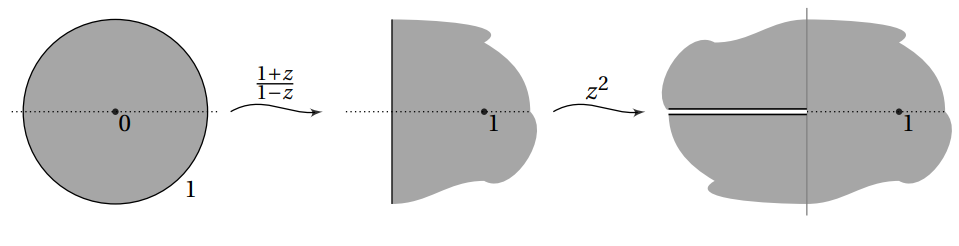
\includegraphics[width=0.8\textwidth]{imagenes/ej4.png}
    \end{align*}
    \item El disco unidad es conformemente equivalente al sector $S_{\alpha} = \{ re^{i\theta} : r > 0, |\theta| < \alpha \}$ de apertura $2\alpha$ ($\alpha \in (0,\pi]$) mediante la aplicación $f_{\alpha}(z) = \left(\frac{1 + z}{1-z} \right)^{\frac{2}{\pi}\alpha}$ y donde se usa la rama principal de la potencia.
    \begin{align*}
        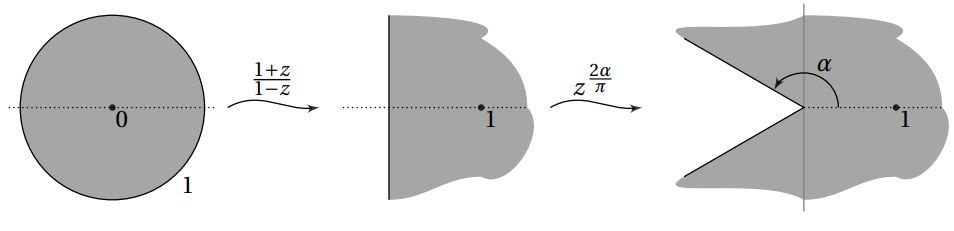
\includegraphics[width=0.8\textwidth]{imagenes/ej5.png}
    \end{align*}
    \item El disco unidad es conformemente equivalente a la banda horizontal $B_{h} = \{ \im |z| < h \}$ de altura $2h$ ($h > 0$), mediante la aplicación $f(z) = \frac{2h}{\pi}\logp\left( \frac{1+z}{1-z}\right)$
    \begin{align*}
        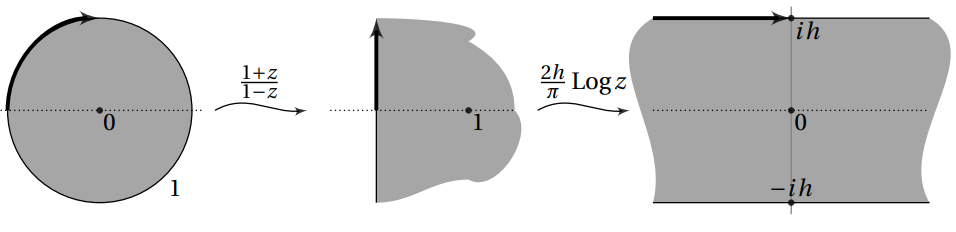
\includegraphics[width=0.8\textwidth]{imagenes/ej6.png}
    \end{align*}
    \item El disco unidad es conformemente equivalente a $\mathbb{H} \backslash [0,1]$, mediante la secuencia de aplicaciones
    \begin{align*}
        &\mathbb{D} \xrightarrow{} \com \backslash (-\infty,0] \xrightarrow{} \com \backslash (-\infty,1] \xrightarrow{} \mathbb{H} \backslash [0,1] \\
        &z \longmapsto \left(\frac{1 + z}{1-z} \right)^2 \longmapsto \bullet + 1 \longmapsto \sqrt{\bullet}
    \end{align*}
    donde nuevamente se ha usado la rama principal de la raíz cuadrada.
    \begin{align*}
        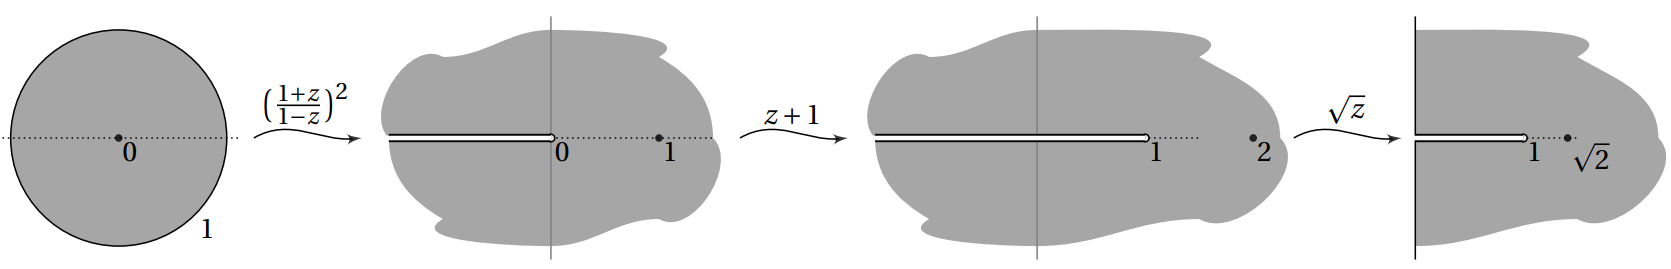
\includegraphics[width=1\textwidth]{imagenes/ej7.png}
    \end{align*}
    \item El disco unidad es conformemente equivalente a $\mathbb{D} \backslash [-1,0]$, usando la aplicación $\sqrt{\left( \frac{1+z}{1-z}\right)^2 + 1}$, $z \in \mathbb{D}$ y luego la inversa de la aplicación de Cayley, $\frac{w-1}{w+1}$, $w \in \mathbb{H}$. Así, una aplicación conforme entre $\mathbb{D}$ y $\mathbb{D} \backslash [-1,0]$ es
    \begin{align*}
        f(z) = \frac{\sqrt{\left( \frac{1+z}{1-z}\right)^2 + 1} -1}{\sqrt{\left( \frac{1+z}{1-z}\right)^2 + 1} + 1}
    \end{align*}
    donde $z \in \mathbb{D}$.
    \begin{align*}
        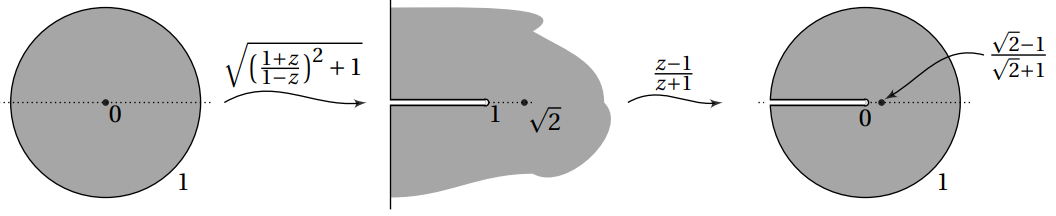
\includegraphics[width=0.8\textwidth]{imagenes/ej8.png}
    \end{align*}
    \item El disco unidad es conformemente equivalente a $\mathbb{D} \backslash \overline{\Delta\left( \frac{1}{2}, \frac{1}{2}\right)}$. La secuencia de aplicaciones sería así
    \begin{align*}
        &\mathbb{D} \xrightarrow{} \mathbb{H} \xrightarrow{} \{  0 < \im z < 1\} \xrightarrow{} \{  0 < \re z < 1\} \xrightarrow{} \overline{\Delta\left( \frac{1}{2}, \frac{1}{2}\right)} \\
         &z \longmapsto \frac{1+z}{1-z} \longmapsto \frac{1}{\pi} \logp(\bullet) + \frac{i}{2} \longmapsto i(\bullet) + 1 \longmapsto\frac{\bullet - 1}{\bullet +1}
    \end{align*}
    \begin{align*}
        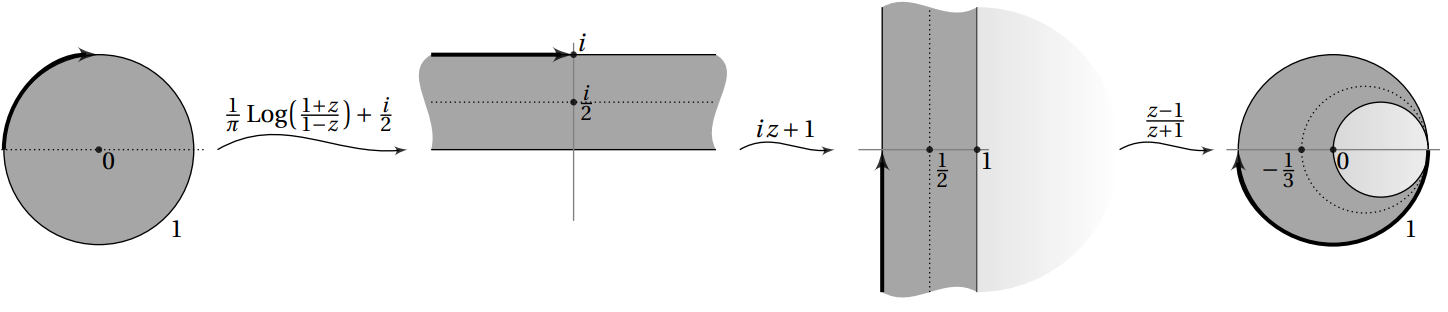
\includegraphics[width=1\textwidth]{imagenes/ej9.png}
    \end{align*}
\end{enumerate}
\end{ejemplo}
\chapter{Cambio de variable}

\section{Cambio de variable (variable discreta)}

\begin{prop}
    Sea X una variable aleatoria discreta y sea $D_X = \{x_n\}$ el conjunto de puntos de salto con $\{P_X(\{x_n\})$ función de masa. Sea $Y = g(X)$ con $g$ función medible concentrada en $g(D_X)$. Entonces Y es una variable aleatoria y
    \begin{align*}
        P(Y = y) = \sum_{x_n \in D_x \cap g^{-1}(y)}{P_X(\{x_n\})}.
    \end{align*}
\end{prop}

\section{Cambio de variable (variable absolutamente continua)}
\subsection{Variable aleatoria absolutamente continua a variable aleatoria discreta}

\begin{prop}
    Sea X una variable aleatoria absolutamente continua con función de densidad $f_X$. Sea $g: I \longrightarrow \mathbb{R}$ una función medible que toma a lo sumo un número infinito numerable de valores en $\mathbb{R}$, es decir, $g(I) = \cup_{i \in I}{y_i}$. Entonces $Y = g(X)$ es una variable aleatoria discreta y
    \begin{align*}
        P(Y = y_i) = P(g(X) = y_i) = P(X \in g^{-1}(y_i)).
    \end{align*}
\end{prop}

\subsection{Variable aleatoria absolutamente continua a variable aleatoria absolutamente continua}

\begin{teo}[Teorema de cambio de variable]
    Sea X una variable aleatoria absolutamente continua con función de densidad $f_X$ concentrada en un intervalo $I \subseteq \mathbb{R}$. Sea $g: I \longrightarrow \mathbb{R}$ una función medible, derivable, con derivada continua y estrictamente monótona. Entonces $Y = g(x)$ es variable aleatoria absolutamente continua con función de densidad
    \begin{align*}
        f_Y(y) = f_X(g^{-1}(y)) \cdot |(g^{-1}(y))'|.
    \end{align*}
\end{teo}

\begin{proof}
    Supongamos que $g$ es estrictamente creciente. Consideremos $Y = g(X)$. $Y$ es una variable aleatoria absolutamente continua si existe $h: \mathbb{R} \longrightarrow \mathbb{R}$ no negativa, integrable-Riemann en [a,b], $a,b \in \mathbb{R}$ y $\int_{-\infty}^{+\infty}{h(y) \ dy} = 1$.

    Si $h$ es la función de densidad de $Y$, entonces debe verificar
    \begin{align*}
        P_Y((a,b]) = F_Y(b) - F_Y(a) = \int_{a}^{b}{h(x) \ dy}.
    \end{align*}
    Construyamos $h$.
    \begin{align*}
        P_Y((a,b]) = P_Y(a < Y \leq b) = P(a < g(X) \leq b).
    \end{align*}
    Como $g$ es estrictamente creciente
    \begin{align*}
        P(a < g(X) \leq b) & = P(g^{-1}(a) < X \leq g^{-1}(b)) = \int_{g^{-1}(a)}^{g^{-1}(b)}{f_X(x) \ dx} \\
                           & = \int_{g^{-1}(a)}^{g^{-1}(b)}{f_X(g^{-1}(y)) \cdot |(g^{-1}(y))'|\ dy}       \\
                           & = \int_{g^{-1}(a)}^{g^{-1}(b)}{f_X(g^{-1}(y)) \cdot (g^{-1}(y))'\ dy}
    \end{align*}
    Definimos $h = f_X(g^{-1}(y)) \cdot (g^{-1}(y))'$. Es claro que $h \ge 0$ y que $\int_{-\infty}^{+\infty}{h(y) \ dy} = 1$. Por tanto $h$ es función de densidad de probabilidad.

    El caso de $g$ estrictamente decreciente se hace de forma análoga.
\end{proof}

\begin{teo}[Generalización del teorema de cambio de variable]
    Sea X una variable aleatoria absolutamente continua con función de densidad $f_X$ y sea $g$ una función medible con dominio $I = \cup_{i=1}^{n}{D_i}$, de forma que $g_i = g|_{D_i}$ es estrictamente monótona en cada $D_i$, diferenciable y con derivada no nula. Entonces $Y = g(X)$ es variable aleatoria absolutamente continua con función de densidad
    \begin{align*}
        f_Y(y) = \sum_{y \in g_i(D_i)}{f_X(g_i^{-1}(y)) \cdot |(g_i^{-1}(y))'|}.
    \end{align*}
\end{teo}

\subsection{Variable aleatoria absolutamente continua a variable aleatoria mixta}

\begin{prop}
    Sea X una variable aleatoria absolutamente continua con función de densidad $f_X$ y sea $g$ una función medible constante a lo sumo en un número infinito numerable de intervalos de $\mathbb{R}$ y continua en al menos un intervalo de $\mathbb{R}$. Entonces $Y = g(X)$ es una variable aleatoria con distribución mixta.
\end{prop}

\section{Variables aleatorias truncadas}

\begin{defi}
    Sea X una variable aleatoria y sea $P_X$ la distribución de pobabilidad inducida por $X$ en $\mathbb{R}$. Entonces $Y = X | X \in T$ donde $T \in \mathbb{B}_1$ es una variable aleatoria truncada.
\end{defi}

\begin{obs}
    Si $X$ es una variable aleatoria y $P_X$ la distribución de pobabilidad inducida por $X$ en $\mathbb{R}$. Consideramos $Y = X | X \in T$ donde $T \in \mathbb{B}_1$. Entonces
    \begin{align*}
        P_Y(B) = P(Y \in B) = P(X \in B \ | \ X \in T) = \frac{P_X(B \cap T)}{P_X(T)}.
    \end{align*}
\end{obs}

\begin{prop}
    Sea X una variable aleatoria con función de distribución $F_X$. Entonces
    \begin{enumerate}
        \item[(i)] La variable aleatoria $Y = X | X \ge x_0$, $x_0 \in \mathbb{R}$, $T = [x_0,+\infty)$ tiene como función de distribución
              \begin{align*}
                  F_1(y) = \left\{ \begin{array}{lcc}
                                       0                                          & si & y < x_0   \\
                                       \frac{F_X(y) - F_x(x_0^-)}{1 - F_X(x_0^-)} & si & y \ge x_0 \\
                                   \end{array}
                  \right.
              \end{align*}
        \item[(ii)] La variable aleatoria $Y = X | X \leq x_0$, $x_0 \in \mathbb{R}$, $T = (-\infty,x_0]$ tiene como función de distribución
              \begin{align*}
                  F_2(y) = \left\{ \begin{array}{lcc}
                                       \frac{F_X(y)}{F_X(x_0)} & si & y < x_0   \\
                                       1                       & si & y \ge x_0 \\
                                   \end{array}
                  \right.
              \end{align*}
        \item[(iii)] La variable aleatoria $Y = X | x_0 \leq X < x_1$, $x_0,x_1 \in \mathbb{R}$, $T = [x_0,x_1)$ tiene como función de distribución
              \begin{align*}
                  F_3(y) = \left\{ \begin{array}{lcc}
                                       0                                                   & si & y < x_0          \\
                                       \frac{F_X(y) - F_x(x_0^-)}{F_X(x_0^-) - F_X(x_1^-)} & si & x_0 \leq y < x_1 \\
                                       1                                                   & si & y \ge x_1        \\
                                   \end{array}
                  \right.
              \end{align*}
    \end{enumerate}
\end{prop}
\chapter{El Teorema del Cambio de Variables}

\begin{prop}
Sea $T: \mathbb{R}^n \longrightarrow \mathbb{R}^n$ un isomorfismo lineal y sea A un conjunto medible-Borel. Entonces T(A) es medible-Borel y $m(T(A)) = |det(T)|m(A)$.
\end{prop}

\begin{proof}
Ya sabemos que $T(A)$ es medible-Borel. Veamos la igualdad.
\\
\newline
Caso I. Supongamos que
\begin{align*}
    T(x_1,...,x_j,...,x_n) = (x_1,...,x_{j-1},cx_j,x_{j+1},...,x_n), \ \ \ c \in \mathbb{R}, c \not = 0.
\end{align*}
Es claro que $\det(T) = c$. Para este caso, ya vios que 
\begin{align*}
    |1| \cdots |1|\cdot |c| \cdot |1| \cdots |1|m(A) = |det(T)|m(A).
\end{align*}
Caso II. Supongamos que existen $j, k \in \{1,...,n\}$, $j \not = k$ y $c \in \mathbb{R}$ tales que
\begin{align*}
    T(x_1,...,x_j,...,x_n) = (x_1,...,x_{j-1},x_j +cx_k,x_{j+1},...,x_n).
\end{align*}
Es claro que $|\det(T)| = 1$. Por comodidad en la demostración, vamos a suponer que $j = 1$. Así
\begin{align*}
    T(x_1,x_2,...,x_n) = (x_1 +cx_k,x_2,...,x_n).
\end{align*}
Consideramos que $\mathbb{R}^n = \mathbb{R} \times \mathbb{R}^{n-1}$ y aplicamos el Principio de Cavalieri
\begin{align*}
    m(T(A)) = \int_{\mathbb{R}^{n-1}}{m(T(E))^{(x_2,...,x_n)}) \ dm_{n-1}(x_2,...,x_n)}.
\end{align*}
Ahora bien,
\begin{align*}
    (T(A))^{(x_2,...,x_n)} &= \{ x \in \mathbb{R} : (x,x_2,...,x_n) \in T(A) \} \\
    &= \{ x \in \mathbb{R} : x = x_1 + cx_k, (x_1,x_2,...,x_n) \in A \} \\
    &= \{x \in \mathbb{R} : x = x_1 + cx_k, x_1 \in A^{(x_2,...,x_n)} \} \\
    &= A^{(x_2,...,x_n)} + cx_k.
\end{align*}
Como la medida de Lebesgue es invariante frente a traslaciones, $m(T(E))^{(x_2,...,x_n)} = m(E^{(x_2,...,x_n)})$. Por lo tanto, aplicando de nuevo el Principio de Cavalieri.
\begin{align*}
    m(T(E)) &= \int_{\mathbb{R}^{n-1}}{m(T(A))^{(x_2,...,x_n)}) \ dm_{n-1}(x_2,...,x_n)} \\
    &= \int_{\mathbb{R}^{n-1}}{m(A^{(x_2,...,x_n)}) \ dm_{n-1}(x_2,...,x_n)} = m(A).
\end{align*}
Por tanto, $m(T(A)) = |1|\cdot m(A)$.
\\
\newline 
Caso III. Sea $T$ ahora un isomorfismo lineal cualquiera. Entoces existen $T_1,...,T_s$ isomorfisos lineales de los tipos contemplados en los casos I y II tales que  $T = T_1 \circ \cdots \circ T_s$. Así
\begin{align*}
    m(T(A)) &= m(T_1(T_2(...(T_s(A))))) = |\det(T_1)|m(T_2(T_3(...(T_s(A))) \\
    &= |\det(T_1)| \cdots |\det(T_s)|m(A) = |\det(T)|m(A).
\end{align*}
\end{proof}

\begin{prop}
Sea $T: \mathbb{R}^n \longrightarrow \mathbb{R}^n$ un isomorfismo lineal y sea A un conjunto medible-Lebesgue. Entonces T(A) es medible-Lebesgue y $m(T(A)) = |det(T)|m(A)$.
\end{prop}

\begin{proof}
Supongamos en primer lugar que $m(A) = 0$. Entonces existe un conjunto medible-Borel $G$ tal que $A \subset G$ y $m(G) = 0$. Por la proposición anterior, $m(T(G)) = 0$, y como $T(A) \subset T(G)$, se tiene que $T(A)$ es medible-Lebesgue y $m(T(A)) = 0$, lo que prueba la proposición en este caso.
\\
\newline
Supongamos ahora que $A$ es un conjunto medible-Lebesgue cualquiera. Entonces, existen un conjunto medible-Borel $B$ y un conjuto medible-Lebesgue $N$ tales que
\begin{align*}
    A = B \cup N \text{ y } m(N) = 0 \text{ y, en consecuencia, } m(A) = m(B).
\end{align*}
Entonces,
\begin{align*}
    T(A) = T(B) \cup T(N).
\end{align*}
Por la proposición anterior, $T(B)$ es medible-Borel y $m(T(B)) = |\det(T)|m(B)$. Por el primer caso de esta proposición, $T(N)$ es medible-Lebesgue y $m(T(N)) = 0$. Como $T(A) = T(B) \cup T(N)$, entonces $T(A)$ es medible-Lebesgue y
\begin{align*}
    m(T(A)) = m(T(B)) = |\det(T)|m(B) = |\det(T)|m(E),
\end{align*}
coom queríamos demostrar.
\end{proof}

\begin{obs}
Si $E$ es medible-Lebesgue entonces $\mathcal{X}_{T(E)}$ es medible-Lebesgue y
\begin{align*}
    \int_{\mathbb{R}^n}{\mathcal{X}_{T(E)} \ dm} = |\det(T)|\int_{\mathbb{R}^n}{\mathcal{X}_{E} \ dm}.
\end{align*}
Aplicando el resultado a $T^{-1}$,
\begin{align*}
    \int_{\mathbb{R}^n}{\mathcal{X}_{T^{-1}(E)} \ dm} = |\det(T^{-1})|\int_{\mathbb{R}^n}{\mathcal{X}_{E} \ dm}.
\end{align*}
Nótese que $\mathcal{X}_{T^{-1}(E)}(x) = \mathcal{X}_{E}{(T(x))}$, obtenemos
\begin{align*}
    \int_{\mathbb{R}^n}{\mathcal{X}_E(T(x)) \ dx} = |\det(T^{-1})|\int_{\mathbb{R}^n}{\mathcal{X}_{E} \ dx} = \frac{1}{|\det(T)|}\int_{\mathbb{R}^n}{\mathcal{X}_{E} \ dx}. 
\end{align*}
Es decir, la igualdad
\begin{align*}
    \boxed{
    \int_{\mathbb{R}^n}{f(x) \ dx} = |\det(T)|\int_{\mathbb{R}^n}{f(T(x)) \ dx},
    }
\end{align*}
es válida para funciones características. Por la linealidad de la integral se sigue que también se da para funciones f simples, medibles y no negativas. Aplicando el Teorema de la Convergencia Monótona concluimos que la igualdad es válida para funciones medibles no negativas. Por último, aplicándolo a las partes positiva y negativa de $f$, concluimos que si $f$ es integrable entonces $g(x) = f(T(x))$ es integrable y la igualdad es válida. El mismo resultado se da para funciones complejas. En realidad, se observa que $f$ es integrable si y sólo si $g(x) = f(T(x))$ es integrable.
\\
\newline
En conclusión, la igualdad es válida para $f$ integrable o $f$ medible no negativa. Dicha igualdad es el Teorema del cambio de variable para transformaciones lineales. En la próxima sección daremos el Teorema para aplicaciones más generales
\end{obs}

\section{El Teorema del Cambio de Variables}

\begin{teo}[Teorema del Cambio de Variables]
Sea $\Omega$ un abierto de $\mathbb{R}^n$, y sea $G: \Omega \longrightarrow \mathbb{R}^n$ una función inyectiva tal que $G \in \mathscr{C}^1(\Omega, \mathbb{R}^n)$ y $\det(DG(x)) \not = 0$ para todo $x \in \Omega$.
\begin{enumerate}
    \item[(a)] Si $f: G(\Omega) \longrightarrow [0,+\infty]$ es medible entonces $(f \circ G)$ y $(f \circ G)|\det(DG)|$ son medibles en $\Omega$ y
    \begin{align*}
        \int_{G(\Omega)}{f(x) \ dx} = \int_{\Omega}{(f \circ G)(x)|\det(DG(x))| \ dx}.
    \end{align*}
    \item[(b)] Sea $f: G(\Omega) \longrightarrow \rcom$. La función $f$ es integrable en $G(\Omega)$ si y solo si $(f \circ G)|\det(DG)|$ es integrable en $\Omega$ y, en ese caso,
    \begin{align*}
        \int_{G(\Omega)}{f(x) \ dx} = \int_{\Omega}{(f \circ G)(x)|\det(DG(x))| \ dx}.
    \end{align*}
    \item[(c)] Si $E \subset \Omega$ es un conjunto medible, entonces $G(E)$ es medible y
    \begin{align*}
        m(G(E)) = \int_{E}{|\det(DG(x))| \ dx}.
    \end{align*}
    \item[(d)] Si $E \subset \Omega$ es un conjunto medible, y $f: G(\Omega) \longrightarrow \mathbb{R}$ es medible no negativa entonces $(f \circ G)$ y $(f \circ G)|\det(DG)|$ son medibles en $E$ y 
    \begin{align*}
        \int_{G(E)}{f(x) \ dx} = \int_{E}{(f \circ G)(x)|\det(DG(x))| \ dx}.
    \end{align*}
     \item[(e)] Sean $E \subset \Omega$ un conjunto medible y $f: G(E) \longrightarrow \mathbb{R}$. La función $f$ es integrable en $G(E)$ si y solo si $(f \circ G)|\det(DG)|$ es integrable en $E$ y, en ese caso,
    \begin{align*}
        \int_{G(E)}{f(x) \ dx} = \int_{E}{(f \circ G)(x)|\det(DG(x))| \ dx}.
    \end{align*}
\end{enumerate}
\end{teo}

\section{Cambio de variables afín}
Sea $b \in \mathbb{R}^n$ y sea $T: \mathbb{R}^n \longrightarrow \mathbb{R}^n$ lineal e invertible. Sea $G : \mathbb{R}^n \longrightarrow \mathbb{R}^n$, $G(t) = b + T(t)$. Por lo tanto, $\det(DG(t)) = \det(T)$. Aplicando el cambio de variables para $f: \mathbb{R}^n \longrightarrow \mathbb{R}$ medible y no negativa o integrable, tenemos
\begin{align*}
    \int_{\mathbb{R}^n}{f(x) \ dx} = \int_{\mathbb{R}^n}{f(b + T(t))|\det(T)| \ dt} = |\det(T)|\int_{\mathbb{R}^n}{f(b + T(t)) \ dt}.
\end{align*}

\section{Coordenadas esféricas}

\subsection{Coordenadas polares en $\mathbb{R}^2$}

El cambio a coordenadas polares toma la forma siguiente:
\begin{align*}
    x_1 &= \rho \cos(\varphi) \\ 
    x_2 &= \rho \sen(\varphi),
\end{align*}
donde $(\rho, \varphi) \in \Delta_2 = (0,+\infty)\times(-\pi,\pi)$. En los términos del teorema de cambio de variables, estamos haciendo lo que sigue. Definimos y $\Phi_2 : \Delta_2 \longrightarrow \mathbb{R}^2$ como
\begin{align*}
    \Phi_2(\rho, \varphi) = (\rho \cos(\varphi), \rho \sen(\varphi)).
\end{align*}
Es fácil ver que $\det(D\Phi_2(\rho, \varphi)) = \rho > 0$.

\subsection{Coordenadas esféricas en $\mathbb{R}^3$}
El cambio a coordenadas esféricas toma la forma siguiente:
\begin{align*}
    x_1 &= \rho \cos(\varphi_1) \\
    x_2 &= \rho \sen(\varphi_1) \cos(\varphi_2) \\
    x_3 &= \rho \sen(\varphi_1) \sen(\varphi_2), 
\end{align*}
donde $(\rho, \varphi_2, \varphi_2) \in \Delta_3 = (0,+\infty)\times(0,\pi)\times(-\pi,\pi)$. En los términos del teorema de cambio de variables, estamos haciendo lo que sigue. Definimos $\Phi_3 : \Delta_3 \longrightarrow \mathbb{R}^3$ como
\begin{align*}
    \Phi_3(\rho, \varphi_1, \varphi_2) = (\rho \cos(\varphi_1), \rho \sen(\varphi_1) \cos(\varphi_2), \rho \sen(\varphi_1) \sen(\varphi_2)).
\end{align*}
Se puede comprobar que $\det(D\Phi_3(\rho, \varphi_1, \varphi_2)) = \rho^2 \sen(\varphi_1) > 0$.

\subsection{Coordenadas esféricas en $\mathbb{R}^n$, $n \ge 3$}
El cambio de coordenadas esféricas en $\mathbb{R}^n$, $n \ge 3$ es una generalización de lo visto anteriormente, y toma la forma siguiente:
\begin{align*}
    x_1 &= \rho \cos(\varphi_1) \\
    x_2 &= \rho \sen(\varphi_1) \cos(\varphi_2) \\
        & \vdots \\
    x_{n-1} &=  \rho \sen(\varphi_1) ... \sen(\varphi_{n-2}) \cos(\varphi_{n-2})\\
    x_{n} &=  \rho \sen(\varphi_1) ...\sen(\varphi_{n-2}) \sen(\varphi_{n-1}),
\end{align*}
donde $(\rho, \varphi_1,..,\varphi_{n-2},\varphi_{n-1}) \in \Delta_n = (0,+\infty)\times(0,\pi)^{n-2}\times(-\pi,\pi)$. Definimos $\Phi_n : \Delta_n \longrightarrow \mathbb{R}^n$ como
\begin{align*}
    \Phi_n(\rho, \varphi_1,..,\varphi_{n-2},\varphi_{n-1}) = (x_1,x_2,...,x_{n-1},x_n).
\end{align*}
Se puede comprobar que
\begin{align*}
    \det(D\Phi_n(\rho, \varphi_1,..,\varphi_{n-1})) = \rho^{n-1}\prod_{i=1}^{n-2}{(\sen(\varphi_i))^{n-1-i}} > 0.
\end{align*}

\subsection{La fórmula del cambio de variables simplificada}
Pongamos que
\begin{align*}
    S^{n-1} = (0,\pi)^{n-2}\times(-\pi,\pi).
\end{align*}
Así
\begin{align*}
    \Delta_n = (0,+\infty)\times S^{n-1}.
\end{align*}
Denotemos por $\varphi$ al vector $\varphi_1,...,\varphi_{n-1}$ y sea
\begin{align*}
    s_{n-1} : S^{n-1} \longrightarrow \mathbb{R}, \ \ \ s_{n-1}(\varphi) = \prod_{i=1}^{n-2}{(\sen(\varphi_i))^{n-1-i}}.
\end{align*}
Como se ve, $s_{n-1}(\varphi)$ es independiente de $\varphi_{n-1}$. Con esta notación,
\begin{align*}
    \det(D\Phi_n(\rho,\varphi_1,...,\varphi_{n-1})) = p^{n-1}s_{n-1}(\varphi).
\end{align*}
Luego, el cambio de variables nos dice que para $f \ge 0$ o $f$ integrable
\begin{align*}
    \int_{\mathbb{R}^n}{f(x) \ dx} &= \int_{\Delta_n}{f(\Phi_n(\rho, \varphi))p^{n-1}s_{n-1}(\varphi) \ d(\rho, \varphi)} \\
    &= \int_{0}^{\infty} \rho^{n-1}\left( \int_{S^{n-1}}{f(\Phi_n(\rho, \varphi))s_{n-1}(\varphi) \ d\varphi} \right) \ d\rho \\
    &= \int_{S^{n-1}}  s_{n-1}(\varphi)\left( \int_{0}^{\infty}{\rho^{n-1}f(\Phi_n(\rho, \varphi))(\varphi) \ d\rho} \right) \ d\varphi.
\end{align*}

\subsection{Cálculo de la medida de la bola unidad}
Sea $B(0,1) \subset \mathbb{R}^n$ la bola cerrada (o abierta) de centro 0 y radio 1. Aplicando el cambio de coordenadas esféricas y empleando esta útlima notación,
\begin{align*}
    m(B(0,1)) = \int_{S^{n-1}} s_{n-1}(\varphi)\left( \int_{0}^{1}{\rho^{n-1} \ d\rho} \right) \ d\varphi = \frac{1}{n}\int_{S^{n-1}} s_{n-1}(\varphi) \ d\varphi
\end{align*}
Si ponemos
\begin{align*}
    \omega_n = \frac{1}{n}\int_{S^{n-1}} s_{n-1}(\varphi) \ d\varphi,
\end{align*}
obtenemos que 
\begin{align*}
    m(B(0,1)) = \frac{\omega_n}{n}.
\end{align*}
Se puede comprobar que
\begin{align*}
    \omega_n = \frac{2\pi^{n/2}}{\Gamma\left( \frac{n}{2} \right)}.
\end{align*}
De aquí deducimos que
\begin{align*}
    m(B(0,1)) = \frac{\omega_n}{n} = \frac{\pi^{n/2}}{\frac{n}{2} \Gamma\left( \frac{n}{2} \right)} = \frac{\pi^{n/2}}{\Gamma\left( \frac{n}{2} + 1 \right)}.
\end{align*}
\chapter{Versión homológica del Teorema de Cauchy}

\section{Cadenas y ciclos}

\begin{defi}
    Sea $\Omega$ un abierto de $\com$. Consideramos el conjunto $\mathcal{C}_{\Omega}$ de todas las sumas formales de caminos de $\Omega$, el tipo $\gamma_1 + ... + \gamma_N$, siendo cada $\gamma_j$ caminno en $\Omega$. En $\mathcal{C}_{\Omega}$ definimos la relación $\sim$ como sigue: $(\gamma_1 + ... + \gamma_N) \sim (\sigma_1 + ... + \sigma_M)$ si y solo si
    \begin{align*}
        \sum_{j=1}^{N} \int_{\gamma_j} f(z) \ dz = \sum_{i=1}^{M} \int_{\sigma_i} f(z) \ dz
    \end{align*}
    para toda función
    \begin{align*}
        f : \left(\bigcup_{j=1}^{N} sop(\gamma_j)\right) \cup \left(\bigcup_{i=1}^{M} sop(\sigma_i)\right) \longrightarrow \com
    \end{align*}
\end{defi}

\begin{obs}
    Es claro que esta relación es una relación de equivalencia en $\mathcal{C}_{\Omega}$.
\end{obs}

\begin{defi}
    A los elementos de $\mathcal{C}_{\Omega}$ les llamamos cadenas en $\Omega$. Un ciclo en $\Omega$ es una cadena en $\Omega$ que admite una representación de la forma $\Gamma = \gamma_1 + ... + \gamma_N$, siendo cada $\gamma_j$ un camino cerrado en $\Omega$.
\end{defi}

\begin{obs}
    Dada la naturaleza de la cadena, es imposible definir origen y extremo de una cadena, así como soporte de una cadena: Si $\gamma_1,\gamma_2$ son caminos en $\Omega$, entonces $\gamma_1$ y $\gamma_1 + \gamma_2 + (-\gamma_2)$ representan a la misma cadena y tienen ''soportes'' distintos.
\end{obs}

\begin{obs}
    Sea $\Omega \subseteq \com$ abierto y sea $f: \Omega \longrightarrow \com$. Sea $\Gamma$ una cadena en $\Omega$. Entonces, para cualesquier representación de $\Gamma$ $\gamma_1 + ... + \gamma_N \sim \gamma_1' + ... + \gamma_M'$, $\gamma_j,\gamma_i'$ caminos en $\Omega$, hemos de tener
    \begin{align*}
        \sum_{j=1}^{N} \int_{\gamma_j} f(z) \ dz = \sum_{i=1}^{M} \int_{\gamma_i'} f(z) \ dz
    \end{align*}
    lo que nos lleva a la siguiente definición.
\end{obs}

\begin{defi}
    Definimos la integral de $f$ a lo largo de $\Gamma$ como
    \begin{align*}
        \int_{\Gamma} f(z) \ dz = \sum_{j=1}^{N} \int_{\gamma_j} f(z) \ dz
    \end{align*}
\end{defi}

\begin{defi}
    Sea $\Gamma$ un ciclo en $\com$ representado por $\gamma_1 + ... + \gamma_N$, siendo cada $\gamma_j$ camino cerrado en $\com$. Si $a \in \com \backslash \bigcup_{j=1}^{N} sop(\gamma_j)$, definimos el índice de $a$ respecto de $\Gamma$ como
    \begin{align*}
        n(\Gamma,a) = \frac{1}{2\pi i} \int_{\Gamma} \frac{1}{z-a} \ dz =  \sum_{j=1}^{N} \frac{1}{2\pi i} \int_{\gamma_j} \frac{1}{z-a} \ dz = \sum_{j=1}^{N} n(\gamma_j,a)
    \end{align*}
\end{defi}

\begin{obs}
    Claramente, tenemos las mismas propiedades que teníamos para caminos cerrados, una vez hayamos fijado una representación $\gamma_1 + ... + \gamma_N$ del ciclo $\Gamma$:
    \begin{itemize}
        \item $n(\Gamma,z) \in \mathbb{Z}$ para todo $z\in \com \backslash \bigcup_{j=1}^{N} sop(\gamma_j)$.
        \item $n(\Gamma,\bullet)$ es una función continua en $\com \backslash \bigcup_{j=1}^{N} sop(\gamma_j)$, luego es constante en cada componente conexa de $\com \backslash \bigcup_{j=1}^{N} sop(\gamma_j)$.
        \item $n(\Gamma,z) = 0$ para todo $z$ en la componente conexa no acotada de $\com \backslash \bigcup_{j=1}^{N} sop(\gamma_j)$.
    \end{itemize}
\end{obs}

\begin{defi}
    Sea $\Omega$ abierto de $\com$. Decimos que un ciclo $\Gamma$ en $\Omega$ es homólogo a 0 módulo $\Omega$, denotado como $\Gamma \sim 0 (\text{mód } \Omega)$, si $n(z,\Gamma) = 0$ para todo $z \in \com \backslash \Omega$.

    Decimos que dos ciclos en $\Omega$, $\Gamma_1$ y $\Gamma_2$, son homólogos módulo $\Omega$, si $\Gamma_1 - \Gamma_2 \sim 0 (\text{mód } \Omega).$
\end{defi}

\begin{teo}[Lema de separación]
    Sea $\Omega$ abierto en $\com$ y sea $K$ un compacto en $\Omega$. Entonces existe un ciclo $\Gamma$ en $\Omega \backslash K$ que satisface
    \begin{enumerate}
        \item[(i)] $\Gamma \sim 0 (\text{mód } \Omega)$.
        \item[(ii)] $n(\Gamma,z) = 1$ para todo $z \in K$.
        \item[(iii)] Para toda función holomorfa en $\Omega$ se tiene que
              \begin{align*}
                  \int_{\Gamma} f(\xi) \ d\xi = 0 \ \ \ \text{y} \ \ \ f(z) = \frac{1}{2\pi i}\int_{\Gamma} \frac{f(\xi)}{\xi - z} \ d\xi, \ \ \forall z\in K
              \end{align*}
    \end{enumerate}
\end{teo}

\begin{teo}
    Sea $\Omega$ un abierto en $\com$ y sea $\Gamma$ un ciclo en $\Omega$. Entonces
    \begin{align*}
        \int_{\Gamma} f(z) \ dz = 0 \text{ para toda } f \text{ holomorfa}\Longleftrightarrow \Gamma \sim 0 (\text{mód } \Omega).
    \end{align*}
\end{teo}

\begin{teo}[Fórmulas integrales de Cauchy]
    Sea $\Omega \subseteq \com$ abierto. Sea $f$ holomorfa en $\Omega$ y sea $\Gamma$ un ciclo en $\Omega$ homólogo a 0 módulo $\Omega$. Supongamos que una representación $\Gamma$ es $\gamma_1 + ... + \gamma_N$ siendo cada $\gamma_j$ camino cerrado en en $\Omega$. Entonces, para cada $z \in \com \backslash \cup_{j=1}^{N} sop(\gamma_j)$ y para cada $n \in \mathbb{N} \cup \{0\}$ se tiene
    \begin{align*}
        f^{(n)}(z)n(\Gamma,z) = \frac{n!}{2\pi i} \int_{\Gamma} \frac{f(\xi)}{(\xi - z)^{n+1}} \ d\xi
    \end{align*}
\end{teo}

\begin{proof}
    Sea $z \in \com \backslash \cup_{j=1}^{N} sop(\gamma_j)$ y sea $n \in \mathbb{N} \cup \{0\}$. Al ser $f$ holomorfa en $\Omega$, se tiene que $f$ es analítica en $\Omega$. Por tanto, podemos considerar:
    \begin{align*}
        g(\xi) = \left\{ \begin{array}{lcc}
                             \frac{n!}{2\pi i} \cdot \frac{f(\xi) - \sum_{k=0}^{\infty} \frac{f^{(k)}(z)}{k!}(\xi - z)^k}{(\xi - z)^{n+1}} & si & \xi \in \Omega \backslash \{z\} \\
                             \\ \frac{n!}{2\pi i} \cdot \frac{f^{(n+1)}(z)}{(n+1)!} &  si & \xi = z \\
                         \end{array}
        \right.
    \end{align*}
    Se puede comprobar facilmente que esta función es continua en $\Omega$ y holomorfa, inicialmente en $\Omega \backslash \{z\}$, por lo que, por un resultado anterior, $g$ es holomorfa en $\Omega$. Así, por la versión homológica del Teorema de Cauchy, $\int_{\Gamma} g(\xi) \ d\xi = 0$. Desgranando esta integral, resulta entonces
    \begin{align*}
        \frac{n!}{2\pi i} \int_{\Gamma} \frac{f(\xi)}{(\xi -z)^{n+1}} \ d\xi = \sum_{k=0}^{\infty} \left( \frac{f^{(k)}(z)}{k!}(\xi - z)^k \cdot \frac{n!}{2\pi i} \int_{\Gamma} \frac{1}{(\xi - z)^{n-k+1}} \ d\xi \right) \underset{(*)}{=}
    \end{align*}
    Como $\frac{1}{(\xi - z)^{n-k+1}}$ tiene primitiva si y solo si $n \not = k$, entonces
    \begin{align*}
        \underset{(*)}{=} \frac{f^{(n)}(z)}{n!} \cdot \frac{n!}{2\pi i} \int_{\Gamma} \frac{1}{\xi -z} \ d\xi + 0 = f^{(n)}(z)n(\Gamma,z).
    \end{align*}
\end{proof}

\section{Dominios simplemente conexos}
En su día dimos la definición de dominio simplemente conexo en $\com$, como un dominio $D$ en $\com$ tal que $\com^* \backslash D$ es conexo.

\begin{teo}[Caracterización de dominios simplementes conexos en $\com$]
    Sea $D \subseteq \com$ un dominio. Son equivalentes:
    \begin{enumerate}
        \item[(a)] $D$ es un dominio simplemente conexo en $\com$.
        \item[(b)] Todo ciclo en $D$ es homólogo a 0 módulo $D$.
        \item[(c)] Todo camino cerrado en $D$ es homólogo a 0 módulo $D$.
    \end{enumerate}
\end{teo}

\begin{teo}[Teorema de Cauchy para dominios simplementes conexos]
    Sea $D \subseteq \com$ un dominio simplemente conexo y sean $f$ holomorfa en $D$ y $\gamma$ un camino cerrado o un ciclo en $D$, entonces $\int_{\gamma} f(z) \ dz = 0$.
\end{teo}

\begin{teo}[Fórmula integrales de Cauchy]
    Sea $D \subseteq \com$ un dominio simplemente conexo. Sean $f$ holomorfa en $D$ y $\gamma_1,...,\gamma_N$ caminos cerrados en $D$. Entonces, para cada $z \in D \backslash \bigcup_{j=1}^{N} \gamma_j$ y cada $n \in \mathbb{N} \cup \{0\}$:
    \begin{align*}
        f^{(n)}(z) \sum_{j=1}^{N} n(\gamma_j,z) = \sum_{j=1}^{N} \frac{n!}{2\pi i} \int_{\gamma_j} \frac{f(\xi)}{(\xi -z)^{n+1}} \ d\xi
    \end{align*}
\end{teo}

Con estos resultados para dominios simplemente conexos, podemos dar otras caracterizaciones de estos dominios.

\begin{teo}[Caracterizaciones de dominio simplemente conexo]
    Sea $D \subseteq \com$ un dominio en $\com$. Son equivalentes:
    \begin{enumerate}
        \item[(i)] $D$ es un dominio simplemente conexo en $\com$.
        \item[(ii)] Todo camino en $D$ (ciclo en $D$), $\gamma$, es homólogo a 0 módulo $D$.
        \item[(iii)] $\int_{\gamma} f(\xi) \ d\xi = 0$ para toda función $f$ holomorfa en $D$, y todo camino cerrado $\gamma$ (ciclo) en $D$.
        \item[(iv)] Toda función holomorfa en $D$ tiene primitiva en $D$.
        \item[(v)] Para toda función f holomorfa en $D$, sin ceros en $D$, existe una rama del $\log(f)$ en $D$.
        \item[(vi)] Toda función armónica en $D$ tiene conjugada armónica en $D$.
    \end{enumerate}
\end{teo}

\begin{proof}
    Ya tenemos que $(i) \Longleftrightarrow (ii) \Longleftrightarrow (iii) \Longleftrightarrow (iv) \Longrightarrow (v)$ y que $(iv) \Longrightarrow (vi)$.

    Veamos que $(v) \Longrightarrow (ii)$. Sea $a \not \in D$. La función $f(z) = z-a$, $z \in D$ es holomorfa en $D$, y nunca 0 en $D$. Entonces existe rama del $\log(z-a)$ en $D$, lo que equivale a decir que $\frac{1}{z-a} = \frac{f'}{f}$ tiene primitiva en $D$, y esto, a su vez, equivale a decir que $\int_{\gamma} \frac{1}{z-a} \ dz = 0$ para todo camino cerrado $\gamma$ en $D$. Como $a \not \in D$ ha sido elegido de manera arbitraria, concluimos que todo camino cerrado en $D$ es homólogo a 0 módulo $D$.

    Finalizamos el teorema probando que $(vi) \Longrightarrow (v)$. Sea $f$ holomorfa en $D$, sin ceros en $D$. Entonces $u = \log |f|$ es armónica en $D$, ya que localmente es la parte real de una función holomorfa. Por hipótesis, existe $g$ holomorfa en $D$ tal que $u = \log|f| = \re(g)$ en $D$. Vamos a probar ahora que existe una constante $\beta \in \com$ tal que $e^{g + \beta} = f$, o sea, tal que $g + \beta$ es rama del $\log(f)$ en $D$. Para probarlo, observamos que la función $F(z) = f(z)e^{-g(z)}$, $z \in D$, es holomorfa en $D$, y $|F(z)| = |f(z)|e^{-\re(g)} = |f(z)|e^{-\log|f(z)|} = 1$, $z \in D$. Esto nos dice que $F$ es constante enn $D$, y es una constate $C$ no nula, pues $|F| = 1 \not = 0$ en $D$. Sea $\beta \in \log(C)$. Entonces $f(z)e^{-g(z)} = F(z) = e^{\beta}$, $z \in D$, o sea, $f(z) = e^{g(z) +\beta}$, $z \in D$.
\end{proof}
\chapter{Singularidades aisladas}

\section{Singularidades aisladas}

\begin{defi}
Por una singularidad aislada de una función $f$ entendemos un punto $z_0$ de manera que $f$ está definida y es holomorfa en un entorno perforado de $z_0$, $\Delta(z_0,r) \backslash \{z_0\}$, sin ser a priori holomorfa en todo el entorno $\Delta(z_0,r)$.
\end{defi}

\begin{ejemplo}
\begin{enumerate}
    \item Las funciones $\frac{1}{z}$, $\frac{\sen z}{z}$, $e^{1/z}$ presentan singularidades aisladas en 0, ya que están definidas y son holomorfas en un entorno perforado de 0.
    \item En principio, según la definición, si $f$ es holomorfa en $z_0$, también podría decir que $f$ presenta una singularidad aislada en $z_0$, aunque el interés es decir esto es nulo.
    \item Un primer resultado sobre singularidades aisladas ya lo vimos como consecuencia de la analiticidad de funciones holomorfas: Si $f$ es continua en un abierto $\Omega$ y $f$ es holomorfa en $\Omega \backslash \{p\}$, siendo $p \in \Omega$, entonces $f$ es holomorfa en $\Omega$. O sea, la singularidad de $p$ es evitable si $f$ es continua en $p$.
    \item Hay puntos que también podríamos llamar singularidades pero no aisladas. Por ejemplo, la función $f(z) = \frac{1}{\sen (1/z)}$ presenta singularidades aisladas en los puntos de la forma $a_n = \frac{1}{n\pi}$, $n \in \mathbb{Z} \backslash \{0\}$. El punto $a = 0$ también es ''singularidad'' de $f$, pero al ser límite de singularidades aisladas (no evitables), resulta que no es holomorfa en ningún entorno perforado de 0, por lo que 0 no puede ser singularidad aislada de $f$.
\end{enumerate}
\end{ejemplo}

\begin{defi}
Si $z_0$ es una singularidad de $f$, decimos que es evitable si $f$ admite una extensión holomorfa a todo un entorno de $z_0$. De esta manera, absusando de notación, la extensión holomorfa de $f$ en un entorno de una singularidad aislada evitable, también se suele denominar $f$.
\end{defi}

\begin{teo}[Teorema de Riemann sobre la singularidad evitable]
Sea $z_0$ una singularidad aislada de $f$. Son equivalentes:
\begin{enumerate}
    \item[(i)] $z_0$ es singularidad aislada evitable de $f$.
    \item[(ii)] $f$ admite extensión continua a $z_0$.
    \item[(iii)] Existe $\lim_{z \to z_0} f(z)$ y es finito.
    \item[(iv)] $f$ está acotada en un entorno perforado de $z_0$.
    \item[(v)] $\lim_{z \to z_0} (z-z_0)f(z) = 0$.
\end{enumerate}
\end{teo}

\begin{proof}
Las implicaciones $(i) \Longrightarrow (ii) \Longrightarrow (iii) \Longrightarrow (iv) \Longrightarrow (v)$ son inmediatas. Probemos $(v) \Longrightarrow (i)$.
\\
\newline
Supongamos que $f$ es holomorfa en $\Delta(z_0,R) \backslash \{z_0\}$ y que $\lim_{z \to z_0} (z-z_0)f(z) = 0$. Entonces la función $g: \Delta(z_0,R) \longrightarrow \com$, dada por 
\begin{align*}
    g(z) = \left\{ \begin{array}{lcc}
             (z-z_0)f(z) &  si  & z \in \Delta(z_0,R) \backslash \{z_0\}\\
             0 &  si & z = z_0 \\
             \end{array}
   \right.
\end{align*}
está bien definida y es continua en $\Delta(z_0,R)$, y además es holomrfa en $\Delta(z_0,R) \backslash \{z_0\}$. Por tanto, tenemos que $g$ es holomorfa en $\Delta(z_0,R)$ y tiene un cero en $z_0$. Todo esto implica que $g$ admite una factorización del tipo $g(z) = (z-z_0)h(z)$, con $h$ holomrfa en $\Delta(z_0,R)$. Se sigue entonces que:
\begin{align*}
    h(z) = \frac{(z-z_0)h(z)}{(z-z_0)} = \frac{g(z)}{z-z_0} = f(z), \ \ z \in \Delta(z_0,R) \backslash \{z_0\}
\end{align*}
probando de esta manera que $h$ es una extensión holomorfa de $f$ en $\Delta(z_0,R)$, y así, $z_0$ es singularidad evitable.
\end{proof}

\begin{defi}
Sea $z_0$ una singularidad aislada de $f$.
\begin{itemize}
    \item $z_0$ es evitable si existe $\lim_{z \to z_0} f(z)$ y es finito.
    \item $z_0$ es polo si existe $\lim_{z \to z_0} f(z)$ y vale $\infty$.
    \item $z_0$ es singularidad aislada esencial si no es aislada ni polo ($f$ no tiene límite en $z_0$).
\end{itemize}
\end{defi}

\begin{ejemplo}
\begin{enumerate}
    \item $f(z) = \frac{\sen z}{z}$ tiene una singularidad aislada evitable en $0$.
    \item $f(z) = \frac{1}{(z-z_0)^n}$ tiene un polo en $z = z_0$.
    \item $f(z) = e^{1/z}$ tiene una singularidad esencial en $z = 0$, pues el límite no existe, basta considerar:
    \begin{align*}
        &\lim_{n \to \infty} f\left( \frac{1}{n} \right) = \lim_{n \to \infty} e^n  = \infty \\
        &\lim_{n \to \infty} f\left(- \frac{1}{n} \right) = \lim_{n \to \infty} e^{-n}  = 0
\end{align*}
\end{enumerate}
\end{ejemplo}

\begin{teo}[Orden de un polo]
Sea $z_0$ un polo de $f$. Entonces existe un primer natural $n_0$ tal que $f(z) = (z-z_0)^{n_0}g(z)$ tiene una singularidad aislada evitable en $z_0$ y, además, trás evitar la singularidad, $g$ no se anula en todo un entorno de $z_0$.
\\
\newline
Dicho primer natural se llama orden $z_0$ como polo de $f$.
\end{teo}

\begin{obs}
\begin{enumerate}
    \item $f$ tiene un polo de orden $n_0$ en $z_0$ si y solo si $\frac{1}{f}$ tiene un cero de orden $n_0$ en $z_0$.
    \item Si $\Omega$ es abierto de $\com$, $z_0 \in \Omega$, y $f$ es holomorfa enn $\Omega \backslash \{z_0\}$, siendo $z_0$ polo de $f$ de orden $n_0$, entonces $g(z) = (z-z_0)^{n_0}f(z)$ es holomorfa en $\Omega$ con $g(z_0) \not = 0$.
    \item Si $z_0$ es singularidad aislada de $f$ que es evitable o polo, entonces existe $\lim_{z \to z_0} f(z)$ como valor en $\com^*$, así que definiendo $f(z_0) = \lim_{n \to z_0} f(z) \in \com^*$, obtenemos una extensión de $f$, continua con respecto a la topología de $\com^*$ en un entorno de $z_0$.
\end{enumerate}
\end{obs}

\begin{teo}[Casorati-Weierstrass]
Si $D$ es un dominio en $\com$ y $f$ es holomorfa en $D \backslash \{z_0\}$, siendo $z_0 \in D$ una singularidad aislada esencial de $f$, entonces para $r>0$ tal que $\Delta(z_0,r) \subset D$, se tiene que $f(\Delta(z_0,r) \backslash \{z_0\})$ es denso en $\com$.
\end{teo}

\section{Desarrollos de Laurent}
Sabemos que si $f$ es holomorfa en $z_0$, entonces $f$ es desarrollable en serie de potencias alrededor de $z_0$:
\begin{align*}
    f(z) = \sum_{n=0}^{\infty}{a_n(z-z_0)^n}
\end{align*}
Cuando $z_0$ es una singularidad aislada evitable o un polo de $f$, también obtenemos un desarrollo en serie de potencias de $(z-z_0)$ de la siguiente forma:
\begin{itemize}
    \item Si $z_0$ es singularidad evitable de $f$, la extensión holomorfa de $f$ en $z_0$, que la llamaremos nuevamente $f$, se encarga de proporcionarnos un desarrollo en serie de potencias ''no negativas'' de $(z-z_0)$:
    \begin{align*}
        f(z) = \sum_{n=0}^{\infty}{a_n(z-z_0)^n}
    \end{align*}
    \item Si $z_0$ es un polo de orden $n_0$ de $f$, entonces $(z-z_0)^nf(z)$ tiene una singularidad evitable en $z_0$, y $n_0$ es el primer natural con esta propiedad. Tras evitar la singularidad enn $z_0$, obtenemos
    \begin{align*}
        (z-z_0)^{n_0}f(z) = \sum_{n=0}^{\infty}{b_n(z-z_0)^n}
    \end{align*}
    De aquí se sigue que
    \begin{align*}
        f(z) &= \frac{1}{(z-z_0)^{n_0}}\sum_{n=0}^{\infty}{b_n(z-z_0)^n} = \sum_{n=0}^{\infty}{b_n(z-z_0)^{n-n_0}} \underset{k = n-n_0}{=} \sum_{k=-n_0}^{\infty}{a_k(z-z_0)^k} \\
        &= \frac{a_{-n_0}}{(z-z_0)^{n_0}} + \frac{a_{-n_0 +1}}{(z-z_0)^{n_0-1}} + ... + \frac{a_{-1}}{(z-z_0)} + a_0 + a_1(z-z_0)+ ....
    \end{align*}
\end{itemize}
Cuando $z_0$ sea una singularidad aislada esencial de $f$, veremos aparecer infinitas potencias negativas de $(z-z_0)$.

\begin{teo}[Desarrollos de Laurent]
Sea $a \in \com$, $0 \leq R_1 < R_2 \leq \infty$, y $f$ holomorfa en el anillo $A = A(a;R_1,R_2) = \{ z \in \com : R_1 < |z-a| < R_2\}$. Entonces $f$ admite un desarrollo, llamado desarrollo de Laurent de $f$ en $A$, de la forma:
\begin{align*}
    f(z) = \sum_{n = -\infty}^{\infty}{a_n(z-a)^n}, \ \ z \in A
\end{align*}
siendo la convergencia de la serie absoluta y uniforme en cada compacto de $A$. Además, los coeficientes $a_n$ vienen dados por la fórmula:
\begin{align*}
    a_n = \frac{1}{2\pi i} \int_{\gamma} {\frac{f(\xi)}{(\xi -a)^{n+1}} \ d \xi}
\end{align*}
donde $\gamma$ es cualquier ciclo de $A$ con $n(\gamma,a) = 1$.
\end{teo}

\begin{obs}
Si $\{a_n\}_{n = -\infty}^{\infty}$ es una sucesión, decimos que la serie $\sum_{n=-\infty}^{\infty} a_n$ converge si las dos series $\sum_{n=0}^{\infty} a_n$, $\sum_{n=1}^{\infty} a_{-n}$ convergen. En tal caso, escribimos $\sum_{n=-\infty}^{\infty} a_n = \sum_{n=0}^{\infty} a_n  +\sum_{n=1}^{\infty} a_{-n}$. Decimos que la serie $\sum_{n=-\infty}^{\infty} a_n$ converge absolutamente si $\sum_{n=-\infty}^{\infty} |a_n|$ es convergente.
\\
\newline
Si $S$ es un conjunto, y para cada $n \in \mathbb{Z}$, $f_n$ es una función de $S$ en $\com$, decimos que la serie $\sum_{n=-\infty}^{\infty} f_n$ converge uniformemente en $S$ si las dos series  funcionales $\sum_{n=0}^{\infty} f_n$, $\sum_{n=1}^{\infty} f_{-n}$ convergen uniformemente en $S$. En tal caso, escribimos $\sum_{n=-\infty}^{\infty} f_n = \sum_{n=0}^{\infty} f_n  +\sum_{n=1}^{\infty} f_{-n}$.
\end{obs}

\begin{obs}
\begin{enumerate}
    \item Una consecuencia de la demostración del teorema sobre desarrollos de Laurent, es que $f$ es descompone como $f = f_1 + f_2$, $f_1(z) = \sum_{n=-\infty}^{-1}a_n(z-a)^n$ y $f_2(z) = \sum_{n=0}^{\infty} a_n (z-a)^n$, siendo $f_1$ holomorfa en $\{ z \in \com : |z-a| > R_1 \}$ y $f_2$ holomorfa en $\{ z \in \com : |z-a| < R_2 \}$.
    \item Si $f$ tiene una singularidad aislada en $a$, entonces $f$ es holomorfa en un anillo de la forma $A(a;0,R)$, para algún $R > 0$, y admite un desarrollo de Laurent alrededor de $a$:
    \begin{align*}
        f(z) = \sum_{n=-\infty}^{\infty}{a_n(z-a)^n}, \ \ z \in A(a;0,R)
    \end{align*}
    La serie de potencias negativas, $f_1 = \sum_{n=-\infty}^{-1}a_n(z-a)^n = P_{f,a}(z)$ se llama \textbf{parte principal del desarrollo de Laurent de $f$ en $a$}. Según el aspecto de esta parte prinicipal, obtenemos la siguiente caracterización de singularidades aisladas:
    \begin{enumerate}
        \item $a$ es singularidad evitable de $f$ si y solo si $f_1 \equiv 0$.
        \item $a$ es polo de $f$ de orden $n_0$ si y solo si $f_1$ es un polinomio de grado $n_0$ en la variable $\frac{1}{z-a}$.
        \item $a$ es singlaridad aislada esencial de $f$ si y solo $f_1$ tiene infinitos sumandos.
    \end{enumerate}
    \item Si $f$ tiene una singularidad aislada en $a$, $f$ es holomorfa en $A(a;0,R)$, para algún $R > 0$, y su desarrollo de Laurent es de la forma
        \begin{align*}
        f(z) = \sum_{n=-\infty}^{\infty}{a_n(z-a)^n}, \ \ z \in A(a;0,R)
    \end{align*}
    Si ahora $\gamma$ es un ciclo en $A(a;0,R)$ tal que $n(\gamma,a) = 1$, entonces
    \begin{align*}
        a_{-1} = \frac{1}{2\pi i} \int_{\gamma} f(\xi) \ d \xi
    \end{align*}
    O sea, hablando coloquialmente, $a_{-1}$ es el único coeficiente del desarrollo de Laurent de $f$ en $a$ que sobrevive al integrar $f$ a lo largo de $\gamma$. Recibe el nombre de \textbf{residuo de $f$ en $a$} 
    \begin{align*}
    \boxed{
        Res(f,a) = a_{-1} = \frac{1}{2\pi i} \int_{\gamma} f(\xi) \ d \xi
    }
    \end{align*}
    cualquiera que sea el ciclo $\gamma$ en $A(a,0,R)$ con $n(\gamma,a) = 1$. 
    \begin{enumerate}
        \item Si $a$ es singularidad evitable de $f$, entonces $Res(f,a) = 0$.
        \item Si $a$ es un polo de $f$ de orden $n_0$, entonces
            \begin{align*}
        f(z) = \sum_{n = -n_0}^{\infty}{a_n(z-a)^n}
    \end{align*}
    con lo que
    \begin{align*}
        (z-a)^{n_0}f(z) = \sum_{k = 0}^{\infty}{a_{k-n_0}(z-a)^k}
    \end{align*}
    De donde deducimos que
    \begin{align*}
    \boxed{
        Res(f,a) = a_{-1} = \frac{1}{(n_0-1)!} \frac{d^{n_0-1}}{dz^{n_0 - 1}}\Big|_{z=a} \left[ (z-a)^{n_0}f(z)\right]
    }
    \end{align*}
    \end{enumerate}
\end{enumerate}
\end{obs}

\section{El infinito}

\begin{defi}
Sea $f$ una función holomorfa definida en un entorno de $\infty$, esto es, existe $R>0$ tal que $f$ está definida en $\{z \in \com : |z| > R \}$. Decimos que $f$ es holomorfa en $\infty$ si $f(1/z)$ tiene una singularidad evitable en $0$, o sea, si $f(1/z)$ es holomorfa en $0$. Decimos que $\infty$ es una singularidad aislada (evitable, polo, esencial) de $f$ si $0$ es singularidad aislada (evitable, polo, esencial) de $f(1/z)$.
\end{defi}

\begin{obs}
\begin{enumerate}
    \item Si $f$ tiene una singularidad aislada en $\infty$, entonces $g(\xi) = f(1/\xi)$ tiene una singularidad aislada en $0$, con desarrollo de Laurent en $0$ del tipo:
    \begin{align*}
        g(\xi) = \sum_{n=-\infty}^{\infty}{b_n \xi^n} = \sum_{n=-\infty}^{\infty}{b_{-n} \left(\frac{1}{\xi}\right)^n} 
    \end{align*}
    y parte prinicipal
    \begin{align*}
        g_1(\xi) = \sum_{n=-\infty}^{1}{b_n \xi^n} = \sum_{n=1}^{\infty}{b_{-n} \left(\frac{1}{\xi}\right)^n} 
    \end{align*}
    De esta manera, podemos decir que el desarrollo de Laurent de $f$ en $\infty$ es como sigue
    \begin{align*}
        f(z) = g(1/z) = \sum_{n=-\infty}^{\infty}{b_{-n}z^n} = \sum_{n=-\infty}^{\infty}{a_nz^n}
    \end{align*}
    y su parte prinicipal es
    \begin{align*}
        f_1(z) = g_1(1/z) = \sum_{n=1}^{\infty}{a_nz^n}
    \end{align*}
    o sea, es una serie de potencias centrada en 0 con radio de convergencia $\infty$ (porque tiene que estar definida y ser holomorfa en un entorno ''perforado'' de $\infty$). En consecuencia:
    \begin{enumerate}
        \item $\infty$ es singualaridad evitable si y solo si $f_1 \equiv 0$.
        \item $\infty$ es polo de orden $n_0$ de $f$ si y solo si $f_1(z) = \sum_{n=1}^{n_0}{a_nz^n}$ es un polinomio de grado $n_0$.
        \item $\infty$ es singularidad aislada esencial de $f$ si y solo si $f_1(z) = \sum_{n=1}^{\infty}{a_nz^n}$ es una serie de potencias alrededor de 0, con infinitos sumandos, y radio de convergencia $\infty$. En otras palabras, $\infty$ es singularidad aislada esencial de $f$ si y solo si $f_1$ es una función enntera distinta de un polinomio.
    \end{enumerate}
    \item En virtud de lo anterior:
    \begin{enumerate}
        \item Todo polimomio de grado $N$ tiene un polo de orden $N$ en $\infty$.
        \item $\frac{1}{z^N}$ es holomorfa en $\infty$ y tiene un cero de orden $N$ es $\infty$.
        \item $e^z = \sum_{n=0}^{\infty}{\frac{z^n}{n!}}$ tiene una singularidad esencial en $\infty$, pues su parte principal es $\sum_{n=1}^{\infty}{\frac{z^n}{n!}} = e^z -1$, que es una función entera que no es un polinomio.
        \item $e^{1/z} = \sum_{n=0}^{\infty}{\frac{1}{n!z^n}} = \sum_{n=-\infty}^{0}{\frac{z^n}{(-n)!}}$ tiene una singularidad aislada en $\infty$, con parte principal igual a $0$. Luego, $e^{1/z}$ es holomorfa en $\infty$ (y en $\infty$ vale $1$).
    \end{enumerate}
\end{enumerate}
\end{obs}

\begin{defi}
Si $f$ tiene una sigularidad aislada en $\infty$, y $R$ es tal que $f$ es holomorfa en $\{z \in \com : |z| > R\}$, definimos el residuo de $f$ en $\infty$ como
\begin{align*}
    Res(f,\infty) = - \frac{1}{2\pi i}\int_{|\xi| = r}{f(\xi) \ d\xi}
\end{align*}
cualquiera que sea $r > 0$.
\end{defi}

\begin{obs}
Una forma rápida para calcular el residuo de $f$ en $\infty$ es la siguiente:
\begin{align*}
    Res(f,\infty) = - \frac{1}{2\pi i} \int_{|\xi| = r}{f(\xi) \ d\xi} \underset{\xi = 1/w}{=} \frac{1}{2\pi i}\int_{|w| = 1/r}{f\left(\frac{1}{w}\right)\left(-\frac{1}{w^2}\right) \ dw} = Res\left( -\frac{1}{w}f\left(\frac{1}{w} \right),0 \right)
\end{align*}
\end{obs}

\begin{defi}
Sea $\Omega$ abierto de $\com^*$ y sea $f: \Omega \longrightarrow \com^*$. Decimos que $f$ es meromorfa en $\Omega$ si $f$ es holomorfa en $\Omega$ salvo por polos (y singularidades evitables, como tales, trás evitarlas, dejan de ser singularidades)
\end{defi}

\begin{obs}
Si $f$ es meromorfa en el abierto $\Omega$ de $\com^*$, entonces el conjunto de polos de $f$ no tiene puntos acumulación en $\Omega$. De lo contrario, $f$ tendría ''singularidades no aisladas'' en $\Omega$. Se sigue entonces que el conjunto de polos de $f$, además de no tener puntos de acumulación en $\Omega$, es a lo sumo numerable, y sus putos de acumulación están en $\partial_{\infty} \Omega$.
\end{obs}

\begin{teo}
\begin{itemize}
    \item Si $f$ es holomorfa en $\com^*$, entonces $f$ es constante.
    \item Si $f$ es meromorfa en $\com^*$, entonces $f$ es una función racional.
\end{itemize}
\end{teo}

\section{El teorema de los residuos}

\begin{prop}
Sea $R$ una función racional. Entonces la suma de los residuos de $R$ es $0$.
\end{prop}

\begin{teo}[Teorema de los residuos]
Si $f$ es holomorfa en un abierto $\Omega \subseteq \com$ excepto en $S \subset \Omega$, conjunto de singularidades aisladas (finitas) de $f$ (puede haber singularidades aisladas esenciales), entonces
\begin{align*}
    \frac{1}{2\pi i}\int_{\gamma}{f(z) \ dz} = \sum_{a \in S}{n(\gamma,a)Res(f,a)}
\end{align*}
para todo ciclo $\gamma$ en $\Omega \backslash S$, homólogo a 0 módulo $\Omega$.
\end{teo}

\begin{obs}
El teorema de los residuos engloba todos los resultados importantes vistos hasta ahora.
\begin{enumerate}
    \item \underline{Teorema de Cauchy}: Si $f$ es holomorfa en el abierto $\Omega \subseteq \com$ y $\gamma$ es un ciclo en $\Omega$ homólogo a 0 módulo $\Omega$, entoces $\int_{\gamma}{f(\xi) \ d\xi} = 0$, pues $f$ no tiene singularidades aisladas.
    \item \underline{Fórmula integral de Cauchy}: Si $f$ es holomorfa en el abierto $\Omega \subseteq \com$, $z_0 \in \Omega$ y $\gamma$ es un ciclo en $\Omega \backslash \{z_0\}$ homólogo a 0 módulo $\Omega$, entonces el conjunto de singularidades de $g(z) = \frac{f(z)}{z-z_0}$, $z \in \Omega \backslash \{z_0\}$ es $S = \{z_0\}$, y observamos que $z_0$ es polo simple de $g$, por lo que $Res(g,z_0) = \lim_{z \to z_0} g(z)(z-z_0) = f(z_0)$. De ahí que 
    \begin{align*}
        \frac{1}{2\pi i}\int_{\gamma} \frac{f(\xi)}{\xi - z_0} \ d\xi = \frac{1}{2\pi i} \int_{\gamma} g(\xi) \ d\xi = n(\gamma,z_0)Res(g,z_0) = n(\gamma,z_0)f(z_0)
    \end{align*}
    \item \underline{Fórmula integral de Cauchy para la $n$-ésima derivada}: Si $f$ es holomorfa en el abierto $\Omega \subseteq \com$, $z_0 \in \Omega$, $n \in \mathbb{N}$, y $\gamma$ es un ciclo en $\Omega \backslash \{z_0\}$ homólogo a 0 módulo $\Omega$, entonces el conjunto de singularidades de $g(z) = \frac{f(z)}{(z-z_0)^{n+1}}$, $z \in \Omega \backslash \{z_0\}$ es $S = \{z_0\}$ y observamos que $z_0$ es un polo de $g$ de orden $n+1$. Teniendo en cuenta que el desarrollo de Taylor de $f$ en $z_0$, $f(z) = \sum_{k=0}^{\infty}{a_k (z-z_0)^k}$, nso da el desarrollo de Laurent de $g$ en $z_0$ : 
    \begin{align*}
        g(z) = (z-z_0)^{-n-1}f(z) = \sum_{k=0}^{\infty}{a_k(z-z_0)^{-n-1+k}}
    \end{align*}
    de donde, obtenemos que
    \begin{align*}
        Res(g,z_0) = a_n = \frac{f^{(n)}(z_0)}{n!}
    \end{align*}
    De aquí se sigue que
    \begin{align*}
        \frac{n!}{2\pi i} \int_{\gamma} \frac{f(\xi)}{(\xi - z_0)^{n+1}} \ d\xi = \frac{n!}{2\pi i} \int_{\gamma} g(\xi) \ d\xi = n!n(\gamma,z_0)Res(g,z_0) = n(\gamma,z_0)f^{(n)}(z_0)
    \end{align*}
\end{enumerate}
\end{obs}

\section{Principio del argumento}

\begin{teo}[De la curva de Jordan]
Sea $J$ el soporte de una curva de Jordan en $\com$. Entonces $\com \backslash J$ tiene exactamente 2 componentes conexas y $J$ es la frontera de ambas.
\begin{itemize}
    \item A la componente acotada de $J$ se le llama \textbf{dominio interior de $J$}, y se denota por $I(J)$.
    \item A la componente no acotada de $J$ se le llama \textbf{dominio exterior de $J$}, y se denota por $E(J)$.
\end{itemize}
\end{teo}

Otrs resultados que aceptaremos como válidos (pero que no demostraremos) son los siguientes:
\begin{enumerate}
    \item Si $\gamma$ es un camino de Jordan y $J = sop(\gamma)$, entonces $n(\gamma,z) = 0$ para todo $z \in E(J)$, (tambien escribiremos $n(\gamma,z) = n(J,z)$), mientras que $n(\gamma,z) = 1$ para todo $z \in I(J)$.
    \begin{itemize}
        \item Si $n(\gamma,z) = 1$ para todo $I(J)$, decimos que $J$ está orientado positivamente.
        \item Si $n(\gamma,z) = -1$ para todo $I(J)$, decimos que $J$ está orientado negativamente.
    \end{itemize}
    \item Cuando $J$ es el soporte de un camino de Jordan positivamente orientado, entonces $I(J)$ recibe el nombre de \textbf{dominio de Jordan}. Dicho de otra forma, un dominio $D \subseteq \com$ se dice que es un \textbf{dominio de Jordan}, si $\partial D$ es el soporte de un camino de Jordan positivamente orientado.
    \item Existen curvas de Jordan con área positiva.
\end{enumerate}

\begin{teo}[Principio del argumento]
Sea $J$ el soporte de un camino de Jordan $\gamma$ positivamente orientado. Sea $D$ un dominio simplemete conexo que contiene a $I(J) \cup J$. Sea $f$ meromorfa en $D$ sin ceros ni polos en $J$, entonces
\begin{align*}
    \frac{1}{2\pi i} \int_{\gamma} \frac{f'(\xi)}{f(\xi)} \ d\xi = (*) - (**)
\end{align*}
siendo
\begin{enumerate}
    \item[(*)] el número de ceros de $f$ en $I(J)$ contando multiplicidades.
    \item[(**)] el número de polos de $f$ en $I(J)$ contando multiplicidades.
\end{enumerate}
\end{teo}

\begin{obs}
Bajo las hipótesis del teorema de los residuos, tenemos que
\begin{align*}
    n(f \circ \gamma,0) = \frac{1}{2\pi i}\int_{f \circ \gamma} \frac{1}{w} \ dw = \frac{1}{2\pi} Var_{f \circ \gamma} (\arg(w)) = \frac{1}{2\pi} Var_{\gamma}(\arg(f))
\end{align*}
\end{obs}

\begin{teo}[Propiedad recubridora local de las funciones holomorfas]
Sea $f$ una función holomorfa en $z_0 \in \com$. Sea $w_0 = f(z_0)$ y sea $N \in \mathbb{N}$ el orden de $z_0$ como cero de $f-w_0$. Entonces $f$ es una aplicación $N \longleftrightarrow 1$ en un entorno de $z_0$, queriendo esto decir que existe $R > 0$, tal que si $f$ es holomorfa en $\Delta(z_0,R)$, y tal que para todo $r \in (o,R)$, existe $\delta > 0$ con la propiedad de que si $w \in A(w_0,\delta) \backslash \{w_0\}$, entonces existen $N$ puntos distintos $z_1(w),...,z_N(w) \in \Delta(z_0,r)$ con $f(z_j(w)) = w$, $j = 1,...,N$.
\end{teo}

\begin{cor}[Teoerma de la aplicación abierta]
Si $f$ es meromorfa y no constante, entonces $f$ es una aplicación abierta (en la topologia de $\com^*$).
\end{cor}

\begin{obs}
\begin{enumerate}
    \item Si $f$ es meromorfa y no constante en el abierto $\Omega$, entoncnes $f(\Omega)$ es abierto.
    \item Si $f$ es meromorfa y no constante en el dominio $D$, entonces  $f(D)$ es dominio.
\end{enumerate}
\end{obs}

\begin{teo}[Teorema de Rouché]
Sea $J$ el soporte de un camino de Jordan $\gamma$. Sea $D$ un dominio simplemente conexo en $\com$, satisfaciendo que $I(J) \cup J \subset D$. Sean $f,g$ holomorfas en $D$ y tales que
\begin{align*}
    |f(z) - g(z)| < |g(z)|, \ \ \text{para todo } z \in J.
\end{align*}
Entonces $f$ y $g$ tienen el mismo números de ceros en $I(J)$ (por supuesto, contando multiplicidad).
\end{teo}

\begin{teo}[De Hurwitz (I)]
Supongamos que $\{f_n\}$ es una sucesión de funciones holomorfas en un dominio $D$, que converge normalmente a una función $f$ (que sabemos que es holomorfa en $D$). Entonces. o bien $f \lea 0$ en $D$, o bien cada vez que $z_0 \in D$ sea un cero de orden $N \ge 0$, existen $r_0 > 0$ y $n_0 \in \mathbb{N}$ con la propiedad que, para todo $n \ge n_0$ $f_n$ tiene exactamente $N$ ceros en $\Delta(z_0,r_0)$ contando multiplicidades. Es más, estos ceros convergenn a  $z_0$ en medida que $n \to \infty$.
\\
\newline
En particular, si cada $f_n$ carece de ceros y $f$ no es identicamente cero, entonces $f$ también carece de ceros.
\end{teo}

\begin{teo}[De Hurwitz (II)]
Supongamos que $\{f_n\}$ es ua sucesión de funciones holomorfas e inyectivas en un dominio $D$, que converge normalmente a una función $f$ (que sabemos que es holomorfa en $D$). Entonces, obien $f$ es constante en $D$, o bien $f$ es inyectiva en $D$. 
\end{teo}
\end{document}